%%%%%%%%%%%%%%%%%%%%%%%%%%%%%%%%%%%%%%%%%%%%%%%%%%%%%%%%%%%%%%%%%%%%%%%%%%%%%%%
% documentclass→
\PassOptionsToPackage{full}{textcomp}
\documentclass[a4paper, twoside, nobib]{tufte-book}
\hypersetup{colorlinks}

%%%%%%%%%%%%%%%%%%%%%%%%%%%%%%%%%%%%%%%%%%%%%%%%%%%%%%%%%%%%%%%%%%%%%%%%%%%%%%%
% metadata

\title[ML-based precision medicine in ischemic heart disease]{%
    Machine Learning-Based Precision Medicine in Ischemic Heart Disease}
\author[Peter Christoffer Holm]{Peter Christoffer Holm}
\publisher{%
    Graduate School of Health and Medical Sciences
    University of Copenhagen%
}
% ←
%%%%%%%%%%%%%%%%%%%%%%%%%%%%%%%%%%%%%%%%%%%%%%%%%%%%%%%%%%%%%%%%%%%%%%%%%%%%%%%
% biblatex configuration →

\usepackage[%
    style=verbose-note,
    %%%%%%%%%%%%%%%%%%%%%%%%%%%%%%%%%%%%%%%%%%
    isbn=false,
    doi=false,
    eprint=false,
    date=year,
    maxcitenames=2,     % when should "et al." be triggered?
    maxbibnames=4,      % when should "et al." be triggered? (in bib)
    sorting=nty,        % name, title, year
    autocite=footnote,  % put citation in sidenotes 
    citereset=chapter,  % reset citation tracker at each chapter
    citetracker=strict,
    trackfloats=true,
    autopunct=true
]{biblatex}

\DeclareCiteCommand{\cite}
  {\usebibmacro{prenote}}
  {\usebibmacro{citeindex}%
   \usebibmacro{footcite}}
  {\multicitedelim}
  {\usebibmacro{cite:postnote}}

\newcommand{\sidecite}[2][0em]{%
	\unskip\sidenote[][#1]{\cite{#2}}%
}

\renewbibmacro{in:}{}
\addbibresource{assets/pch-thesis.bib}

\DeclareSourcemap{
    \maps[datatype=bibtex]{
        \map{
            \pertype{incollection}
            \step[fieldset=url, null]
            \step[fieldset=urldate, null]
        }
        \map{
            \pertype{article}
            \step[fieldset=url, null]
            \step[fieldset=urldate, null]
        }
        \map{
            \pertype{book}
            \step[fieldset=url, null]
            \step[fieldset=urldate, null]
        }
        \map{
            \pertype{online}
            \step[fieldsource=eprinttype, final=true]
            \step[typesource=online, typetarget=article]
            \step[fieldsource=eprinttype, fieldtarget=journaltitle]
            \step[fieldsource=journaltitle, match={arxiv}, replace={arXiv}]
            \step[fieldset=urldate, null]
        }
        \map{
            \pertype{inproceedings}
            \step[fieldset=publisher, null=true]
            \step[fieldset=url, null=true]
            \step[fieldset=urldate, null=true]
        }
        \map{
            \pertype{manual}
            \step[fieldset=url, null=true]
            \step[fieldset=urldate, null=true]
        }
        \map{
            \step[fieldset=pages, null]
            \step[fieldset=pagetotal, null]
            \step[fieldset=series, null]
            \step[fieldset=issue, null]
            \step[fieldset=volume, null]
            \step[fieldset=number, null]
            \step[fieldset=location, null]
            \step[fieldset=editor, null]
            \step[fieldset=eprint, null]
        }
        \map{
            \step[fieldsource=url, final=true]
            \step[fieldset=verba, origfieldval, final=true]
            \step[
               fieldsource=verba, 
               match=\regexp{\A(https?...)?(www.)?}, 
               replace={}
            ]
        }
    }
}

\DeclareFieldFormat{url}{%
  \mkbibacro{URL}\addcolon\space
  \href{#1}{\nolinkurl{\thefield{verba}}}}

% ←
%%%%%%%%%%%%%%%%%%%%%%%%%%%%%%%%%%%%%%%%%%%%%%%%%%%%%%%%%%%%%%%%%%%%%%%%%%%%%%%
% load packages →

% fonts
\usepackage[T1]{fontenc}

\usepackage[osf, p]{ETbb}  % osf in text, tabular lining figures in math
\usepackage[scaled=.95,type1]{cabin}  % sans serif in style of Gill Sans
\usepackage[libertine, vvarbb]{newtxmath}
\usepackage[scaled=.90]{FiraMono}

% misc
\usepackage{amsmath}
\usepackage{amsfonts}
\usepackage{microtype}
\usepackage{booktabs}
\usepackage[danish, british]{babel}
\usepackage{multirow}
\usepackage{tabularx}
\usepackage{multicol}
\usepackage{makecell}
\usepackage{pdfpages}
\usepackage{bookmark}
\usepackage[export]{adjustbox}
\usepackage{datetime}

\usepackage[mode=match]{siunitx}
\DeclareSIUnit\year{yr}

\usepackage{subcaption}
\captionsetup{font=footnotesize}    

\usepackage{marginfix}
\usepackage{appendix}
\usepackage{twemojis}
\usepackage{cleveref}
\usepackage{pgffor}
\usepackage{relsize}  % easy scaling of fonts
\usepackage{bm}
\usepackage[morefloats=200]{morefloats}

% enumerate
\usepackage[inline]{enumitem}
\renewlist{enumerate*}{enumerate*}{1}
\setlist[enumerate*]{
    label=(\roman*), itemjoin={{; }}, itemjoin*={{; and }}
}

% context aware quotation marks
\usepackage{csquotes}  
\renewcommand{\mkcitation}[1]{~\autocite{#1}}

% acro 
\usepackage{etoolbox}
\usepackage[nohyperlinks]{acronym}
\renewcommand*{\acsfont}[1]{\textlf{\textsmaller[.5]{#1}}}

\makeatletter
\pretocmd{\@makechapterhead}{\acresetall}{}{}
\makeatother

%% https://tex.stackexchange.com/a/71368/128811
\makeatletter
\newcommand*{\org@overidelabel}{}
\let\org@overridelabel\@verridelabel
\renewcommand*{\@verridelabel}[1]{%
\@bsphack
\protected@write\@auxout{}{\string\AC@undonewlabel{#1@cref}}%
\org@overridelabel{#1}%
\@esphack
}%
\makeatother


% tikz 
\usepackage{tikz}
\usepackage{pgfplots}
\usepgfplotslibrary{groupplots}
\usepackage{listofitems}
\usepackage{contour}
\usepackage[most]{tcolorbox}

\usetikzlibrary{positioning}
\usetikzlibrary{matrix}
\usetikzlibrary{arrows,shapes}
\usetikzlibrary{arrows.meta} 
\usetikzlibrary{graphs} 
\usetikzlibrary{trees} 
\usetikzlibrary{quotes} 
\usetikzlibrary{decorations.text}
\usetikzlibrary{decorations.markings}
\usetikzlibrary{fit}
\usetikzlibrary{babel}

\definecolor{color0}{HTML}{001118}
\definecolor{color1}{HTML}{005e72}
\definecolor{color2}{HTML}{0a9395}
\definecolor{color3}{HTML}{93d1bc}
\definecolor{color4}{HTML}{e8d8a5}
\definecolor{color5}{HTML}{ed9a00}
\definecolor{color6}{HTML}{ca6702}
\definecolor{color7}{HTML}{ba3d02}
\definecolor{color8}{HTML}{ae1f11}
\definecolor{color9}{HTML}{9a2126}

\definecolor{bioc}{HTML}{ebb390}
\definecolor{cln1}{HTML}{e8d19c}
\definecolor{cln2}{HTML}{bfd3e4}
\definecolor{diag}{HTML}{7ba79c}
\definecolor{proc}{HTML}{cadbd8}

% for graphics / images
\usepackage{graphicx}
\setkeys{Gin}{width=\linewidth,totalheight=\textheight,keepaspectratio}
\graphicspath{{graphics/}}

\usepackage{annotate-equations}

% adjust verbatim environments
\usepackage{fancyvrb}
\fvset{fontsize=\normalsize}% ←
%%%%%%%%%%%%%%%%%%%%%%%%%%%%%%%%%%%%%%%%%%%%%%%%%%%%%%%%%%%%%%%%%%%%%%%%%%%%%%%
% custom macros→

% Hanging parentheses and asterisks
\newcommand{\hangp}[1]{\makebox[0pt][r]{(}#1\makebox[0pt][l]{)}}
\newcommand{\hangstar}{\makebox[0pt][l]{*}}

% prints the month name (e.g., january) and the year (e.g., 2008)
\newcommand{\monthyear}{%
  \ifcase\month\or January\or February\or March\or April\or May\or June\or
  July\or August\or September\or October\or November\or
  December\fi\space\number\year
}

% misc
\newcommand{\na}{\quad--}
\newcommand{\blankpage}{\newpage\hbox{}\thispagestyle{empty}\newpage}

\DeclareMathOperator{\EX}{\mathbb{E}} % expected value
\DeclareMathOperator{\PR}{\Pr} % probability 
\DeclareMathOperator{\I}{\mathbb{1}}  % indicator 
\DeclareMathOperator{\CIF}{CIF}
\DeclareMathOperator{\card}{\raisebox{-.22ex}{\#}}

\newcommand{\mat}[1]{\bm{\mathsf{#1}}}
\renewcommand{\vec}[1]{\bm{#1}}

\newcommand{\giv}{\,|\,}
\newcommand{\lik}{\mathscr{l}}
\newcommand{\Lik}{\mathcal{L}}


\newcommand{\Tic}{{T_{\mathrm{c}}}}
\newcommand{\Tid}{{T_{\mathrm{d}}}}
\newcommand{\Cid}{{C_{\mathrm{d}}}}

\newcommand{\tic}{t}
\newcommand{\tid}{\tau}

\DeclareMathOperator*{\argmin}{arg\,min}
\newcommand{\diff}{\mathrm{d}}

\newcommand{\xa}{\mathbf{x}}
\newcommand{\xb}{\check{\xa}}
\newcommand{\hzt}{\lambda_0\mspace{-1mu}(t)}

\newcommand{\pmhnet}[1]{\texttt{PMHnetV#1}}

\newcommand{\studyi  }{\hyperref[chap:study1-outline]{Study I}}
\newcommand{\studyii }{\hyperref[chap:study2-outline]{Study II}}
\newcommand{\studyiii}{\hyperref[chap:study3-outline]{Study III}}


\newcommand{\cbox}[2]{%
    \tcbox[on line, colback=#1, boxsep=1.5pt, colframe=black,
           valign=center, left=0pt, right=0pt, top=0pt, bottom=0pt, boxrule=1pt]{#2}%
}

\DeclareRobustCommand{\uporange}{%
    \begingroup
    \raisebox{-.2\height}{%
      \includegraphics[width=1em]{graphics/upregulated-icon-orange.pdf}%
    }%
    \endgroup
}
\DeclareRobustCommand{\downorange}{%
    \begingroup
    \raisebox{-.2\height}{%
      \includegraphics[width=1em, angle=180, origin=c]%
        {graphics/upregulated-icon-orange.pdf}%
    }%
    \endgroup
}
\DeclareRobustCommand{\upblue}{%
    \begingroup
    \raisebox{-.2\height}{%
      \includegraphics[width=1em]{graphics/upregulated-icon-blue.pdf}%
    }%
    \endgroup
}
\DeclareRobustCommand{\downblue}{%
    \begingroup
    \raisebox{-.2\height}{%
      \includegraphics[width=1em, angle=180, origin=c]%
        {graphics/upregulated-icon-blue.pdf}%
    }%
    \endgroup
}


% ←
%%%%%%%%%%%%%%%%%%%%%%%%%%%%%%%%%%%%%%%%%%%%%%%%%%%%%%%%%%%%%%%%%%%%%%%%%%%%%%%

\iffalse
\includeonly{%
    content/00-copyright.tex,
    content/00-preface.tex,
    content/00-acronyms.tex,
    content/00-summary.tex,
    content/00-manuscripts.tex,
    content/00-overview.tex,
    % content/introduction.tex,
    % content/machine-learning.tex,
    % content/survival-analysis.tex,
    % content/data-foundation.tex,
    % content/study1-outline.tex,
    % content/study2-outline.tex,
    % content/study3-outline.tex,
    content/discussion.tex,
}
\fi

%%%%%%%%%%%%%%%%%%%%%%%%%%%%%%%%%%%%%%%%%%%%%%%%%%%%%%%%%%%%%%%%%%%%%%%%%%%%%%%
\begin{document}

\frontmatter
\kutitlepage
\maketitlepage

\begin{@empty}
~\vfill
\thispagestyle{empty}
\setlength{\parindent}{0pt}
\setlength{\parskip}{\baselineskip}

\smallcaps{Candidate}

\textbf{Peter Christoffer Holm}, MSc

Novo Nordisk Foundation Center for Protein Research,
University of Copenhagen, Denmark

\smallcaps{Supervisors}

\textbf{Søren Brunak}, PhD, Professor 
(principal supervisor)

Novo Nordisk Foundation Center for Protein Research, 
University of Copenhagen, Denmark

\textbf{Henning Bundgaard}, MD, PhD, Professor 
(co-supervisor)

Department of Cardiology,
Copenhagen University Hospital, Denmark

\par\smallcaps{Published by \thanklesspublisher}

\par This document was typeset using latex
using the \texttt{tufte-latex} document class

\par\textit{First printed, \monthyear}

Copyright \copyright\ \the\year\ \thanklessauthor
\end{@empty}
  
\chapter*{Preface}

The work presented in this thesis was performed
at the Novo Nordisk Foundation Center for Protein Research (CPR),
University of Copenhagen, Denmark.

\begin{@empty}
    
\chapter{Summary of Thesis}
\setlength{\parskip}{6pt}

In modern medicine, 
ever increasing amounts of data 
is continuously being generated and recorded. 
Electronic health records,
although not maintained for research purposes,
stands as a unique and valuable source of real-world data
with the potential to revolutionise precision medicine.
This thesis explores the role of \ac{ML} in extracting 
clinically meaningful insights from such large-scale heterogenous health data.
With a primary focus on \ac{IHD},
a global leading cause of morbidity and mortality, 
the thesis presents three original studies 
under the framework of \ac{ML}-based precision medicine.

In \studyi{}, 
we used unsupervised clustering analysis to explore the comorbidity landscape
of \num{72249} patients with \ac{IHD}.
Using the time of the first \acl{CAG} or \acl{CCTA} as the index date,
we defined multimorbidity from the entire spectrum of diagnosis codes
in prior hospital records.
By constructing a patient similarity network from this data, 
we applied the Markov cluster algorithm,
a scalable graph-based clustering method, 
to identify \num{31} distinct clusters 
characterized by distinct patterns of multimorbidity 
and specific risks of subsequent outcomes.
The study's findings can be used to identify knowledge gaps that exist for 
patient subgroups with specific patterns of multimorbidity, 
which are often excluded from clinical trials.

In \studyii{}, 
we present the development and validation of 
a neural network-based survival model
for prediction of all-cause mortality in patients with \ac{IHD}.
This model, \pmhnet{1}, was 
developed using a large and diverse dataset of 
\num{39746} \ac{IHD} patients from the \ac{EDHR}
and incorporates a comprehensive set of 584 features,
including diagnosis history, procedural codes, laboratory test results,
and clinical measurements.
The model's performance was assessed using \ac{tdAUC} and the Brier score, 
and was compared against the \acs{GRACE} risk score 2.0. 
In the test set, \pmhnet{1} demonstrated a \ac{tdAUC} of 0.88 at both six months and one
year, 0.84 at three years, and 0.82 at five years, showing a notably higher
performance than both GRACE2.0 and other simpler models.
External validation on an independent Icelandic dataset of \num{8287} patients 
further showed that the model performance is generalizable.
This study establishes \pmhnet{1} as a valuable tool for assessing
risk of all-cause mortality in a real-world cohort of \ac{IHD} patients,
and can potentially aid clinicians in making informed decisions 
about patient care and interventions.

In \studyiii{}, 
we introduce \pmhnet{2}, an advanced iteration of our 
\ac{IHD} prognostication algorithm.
This updated version predicts three new outcomes,
which includes cause-specific mortality,
new iscemic events, and the development of 
\ac{IHD} complications, including heart failure and 
cardiac arrest.
The study's key contributions are twofold: 
firstly, it presents a novel framework for neural network-based discrete-time 
models capable of modelling time-to-event data with competing risks. 
Secondly, it offers an updated version
of our \acsfont{AI}-driven prognostication tool, 
equipped to predict a broader range of disease-relevant outcomes 
beyond all-cause mortality. 
Our competing-risks framework,
which can be viewed as an extension to discrete-time approach by 
Gensheimer and Narasimhan (2019), 
has been developed into the open-source Python package \textsf{DiscoTime}
(available through PyPI or Github). 
The included manuscript, while still a work in progress, 
effectively showcases the potential and capabilities 
of our proposed methodology and refined models.

\begin{otherlanguage}{danish}
\chapter*{Dansk Resumé}

I moderne medicin genereres og registreres der løbende store mængder data.
Elektroniske patientjournaler 
er ikke oprindeligt designet til at understøtte forskning,
men udgør ikke desto mindre en unik og særdeles værdifuld kilde til
realtidsdata der potentiel kan være med til at revolutionere præcisionsmedicin.
I denne PhD-afhandling undersøger jeg hvordan maskinlæring 
(eng: machine learning) kan anvendes til at 
udtrække klinisk relevant indsigt og mening
fra store databaser indeholdende heterogene sundhedsdata. 
Med hovedfokus på iskæmisk hjertesygdom (IHD),
en globalt ledende årsag til morbiditet og mortalitet, 
præsenterer afhandlingen tre originale studierne
inden for rammerne af maskinlæringsbaseret præcisionsmedicin.

I Studie 1 anvendte vi uovervåget klyngeanalyse til at udforske 
sammensætningen af multimorbiditet hos \num{72249} patienter med IHD. 
Ved at bruge tidspunktet for patienternes første koronarangiografi eller 
koronar-CT som indexdato, 
definerede vi multimorbiditet fra hele spektret af tidligere 
registrerede diagnosekoder fra de patienternes hospitalsjournaler. 
På baggrund af disse data, konstruerede vi et patientsimilaritetsnetværk 
og anvendte derefter Markov-klyngealgoritmen, 
en skalerbar klyngemetode til grafstrukturer, 
til at identificere 31 distinkte patientundergrupper. 
Disse undergrupper var karakteriseret ved at have forskellige 
multimorbiditetsmønstre og tilhørende sygdomsrisici.
Studiets resultater kan bruges til at kortlægge klinisk relevante 
multimorbiditetsmønstre, hvilket kan bruges til at identificere 
patientundergrupper, der lider under multimorbiditet,
og som oftest udelades fra kliniske forsøg og derved reelt 
set ikke dækkes af eksisterende kliniske retningslinjer.


I Studie 2 præsenterer vi udviklingen og valideringen af en dybt neural
netværksbaseret overlevelsesmodel til forudsigelse af alleårsmortalitet hos
patienter med IHD. Denne model, PMHNet-1, blev udviklet ved hjælp af et stort
og mangfoldigt dataset af 39.746 IHD-patienter fra EDHR og inkorporerer et
omfattende sæt af 584 funktioner, herunder diagnosehistorie, procedurekoder,
laboratorieresultater og kliniske målinger. Modellens præstation blev vurderet
ved hjælp af tdAUC og Brier-scoren og sammenlignet med GRACE risikoscore 2.0. I
testsæt demonstrerede PMHNet-1 en tdAUC på 0,88 ved både 6 måneder og et år,
0,84 ved tre år og 0,82 ved fem år, hvilket viste en betydeligt højere
præstation end både GRACE2.0 og andre enklere modeller. Ekstern validering på
et uafhængigt islandsk dataset af 8287 patienter viste yderligere, at
modelpræstationen er generaliserbar. Denne undersøgelse fastslår PMHNet-1 som
et værdifuldt værktøj til at vurdere risikoen for alleårsmortalitet i en
realistisk kohorte af IHD-patienter og kan potentielt hjælpe klinikere med at
træffe informerede beslutninger om patientpleje og interventioner.

I Studie 3 introducerer vi PMHNet-2, en avanceret iteration af vores
IHD-prognostik algoritme. Denne opdaterede version forudsiger tre nye
resultater, herunder årsagspecifik mortalitet, nye iskæmiske hændelser og
udviklingen af IHD-komplikationer, herunder hjertesvigt og hjertestop. Studiets
hovedbidrag er tofoldigt: For det første præsenterer det en ny ramme for dybt
neural netværksbaserede diskrete tid modeller, der er i stand til at modellere
tid-til-begivenhedsdata med konkurrerende risici. For det andet tilbyder det en
opdateret version af vores AI-drevne prognosticeringsværktøj, der er udstyret
til at forudsige et bredere udvalg af sygdomsrelaterede resultater ud over
alleårsmortalitet. Vores konkurrerende risikoramme, som kan betragtes som en
udvidelse af diskret-tidsmetoden af Gensheimer og Narasimhan (2019), er blevet
udviklet til den åbne kildekode Python-pakke DiscoTime (tilgængelig via PyPI
eller Github). Det inkluderede manuskript, selvom det stadig er et arbejde i
gang, viser effektivt potentialet og mulighederne for vores foreslåede metode
og raffinerede modeller.
    
\end{otherlanguage}
\end{@empty}
        
\chapter*{List of Manuscripts}
\section*{Manuscripts included in this thesis}


\subsection*{Manuscript for Study I}

\marginnote[7.5em]{%
  An asterisk (*) denotes equal contribution. \\
  \noindent
  This manuscript was also included in the thesis of Amalie D. Haue.%
}
{\small
\begin{tabularx}{\textwidth}{lX}
    title: & 
    \enquote{%
        Subgrouping multimorbid patients with ischemic heart disease 
        by means of unsupervised clustering: 
        a cohort study of 72,249 patients 
        defined comprehensively by diagnoses prior to presentation%
    } \\
    authors: &
    \raggedright\arraybackslash
    Amalie D. Haue*, \underline{Peter C. Holm}*,
    Karina Banasik, Agnete T. Lundgaard, Victorine P. Muse, Timo Röder, 
    David Westergaard, Piotr J. Chmura, Alex H. Christensen, Peter E. Weeke, 
    Erik Sørensen, Ole B. V. Pedersen, Sisse R. Ostrowski, Kasper K. Iversen, 
    Lars V.  Køber, Henrik Ullum, Henning Bundgaard, 
    and Søren Brunak \\
    preprint: & medRxiv (2023):
    \href{https://doi.org/10.1101/2023.03.31.23288006}%
         {10.1101/2023.03.31.23288006} \\
    status & Submitted (under revision)
\end{tabularx}
}

\subsection*{Manuscript for Study II}

\marginnote[7.5em]{%
  An earlier version of this manuscript was also included 
  in the thesis of Amalie D. Haue.%
}
{\small
\begin{tabularx}{\textwidth}{lX}
    title: & 
    \enquote{%
        Development and validation of a neural network-based survival model 
        for mortality in ischemic heart disease%
    } \\
    authors: &
    \raggedright\arraybackslash
    \underline{Peter C. Holm},
    Amalie D. Haue,  David Westergaard, Timo Röder, Karina Banasik, Vinicius
    Tragante, Alex H. Christensen,  Laurent Thomas,  Therese H. Nøst,
    Anne-Heidi Skogholt, Kasper K. Iversen, Frants Pedersen, Dan E. Høfsten,
    Ole B. Pedersen,  Sisse Rye Ostrowski, Henrik Ullum, Mette N. Svendsen,
    Iben M. Gjødsbøl, Thorarinn Gudnason, Daníel F. Guðbjartsson,  Anna
    Helgadottir, Kristian Hveem,  Lars V. Køber,  Hilma Holm, Kari Stefansson,
    Søren Brunak,  and Henning Bundgaard:
    \\
    preprint: & medRxiv (2023):
    \href{https://doi.org/10.1101/2023.06.16.23291527v1}%
         {10.1101/2023.06.16.23291527v1} \\
    status & Submitted (under review, 2nd round)
\end{tabularx}}

\subsection*{Manuscript for Study III}

{\small
\begin{tabularx}{\textwidth}{lX}
    title: & 
    \enquote{%
        Development of a neural network-based competing risk model 
        for individualized prognostication in ischemic heart disease 
        using a large database of electronic health records 
        and clinical registries}
    \\
    authors: &
    \raggedright\arraybackslash
    \underline{Peter C. Holm},
    Søren Brunak, and Henning Bundgaard
    \\
    preprint: & None \\
    status & Work-in-progress
\end{tabularx}}

\clearpage
\section*{Manuscripts co-authored but not included in this thesis}

\begin{enumerate}

    \item %
    Isa K. Kirk, \ldots, 
    \underline{Peter C. Holm},
    \ldots, Søren Brunak
    \textbf{\enquote{%
        Linking glycemic dysregulation in diabetes to symptoms, 
        comorbidities, and genetics through EHR data mining
    }}
    in \textit{eLife} (2019)

    \item %
    Ina H. Laursen, \ldots, 
    \underline{Peter C. Holm},
    \ldots, Henrik Ullum
    \textbf{\enquote{%
        Cohort profile: Copenhagen Hospital Biobank - Cardiovascular Disease Cohort
        (CHB-CVDC): Construction of a large-scale genetic cohort to facilitate a
        better understanding of heart diseases
    }}
    in \textit{BMJ Open} (2021)

    \item %
    Amalie D. Haue, \ldots, 
    \underline{Peter C. Holm},
    \ldots, Henning Bundgaard, and Søren Brunak
    \textbf{\enquote{%
        Temporal patterns of multi-morbidity in 
        570157 ischemic heart disease patients: 
        a nationwide cohort study
    }}
    in \textit{Cardiovascular Diabetology} (2022)

    \item %
    Alex W. Jung, 
    \underline{Peter C. Holm}, \ldots, 
    Søren Brunak, and 
    Moritz Gerstung
    \textbf{\enquote{%
        Multi-cancer risk stratification based on national health data: a
        retrospective modelling and validation study
    }}
    preprint in \textit{medRxiv} (2022)

    \item %
    Karina Banasik, \ldots, 
    \underline{Peter C. Holm}, \ldots, 
    Thomas F. Hansen
    \textbf{\enquote{%
        DanMAC5: a browser of aggregated sequence variants from 8,671 whole genome
        sequenced Danish individuals
    }}
    in \textit{BMC Genomic Data} (2023)

    \item %
    David Westergaard, \ldots, 
    \underline{Peter C. Holm}, \ldots, 
    Søren Brunak, and 
    Henriette S. Nielsen
    \textbf{\enquote{%
        Immune Changes in Pregnancy: Associations with Pre-existing Conditions and
        Obstetrical Complications at the 20th Gestational Week-A Prospective Cohort
        Study
    }}
    preprint in \textit{medRxiv} (2023)
\end{enumerate}




        

\cleardoublepage

\tableofcontents
\listoffigures
\listoftables

\chapter*{List of Acronyms}
\begin{acronym}[NOMESCO]
\acro{IHD}{ischemic heart disease}
\acro{MI}{myocardial infarction}
\acro{UA}{unstable angina}
\acro{ECG}{electrocardiogram}
\acro{NSTEMI}{non-ST-elevation myocardial infarction}
\acro{STEMI}{ST-elevation myocardial infarction}
\acro{CABG}{coronary artery bypass grafting}
\acro{PCI}{percutaneous coronary intervention}
\acro{CAG}{coronary angiography}
\acroplural{CAG}[CAGs]{coronary angiographies}
\acro{MACE}{major adverse cardiovascular event}
\acro{EHR}{electronic health record}
\acro{CCS}{Canadian Cardiovascular Society}

\acro{PK}{pharmacokinetics}
\acro{SNP}{single-nucleotide polymorphism}
\acro{EHR}{electronic health record}
\acro{ML}{machine learning}
\acro{NLP}{natural language processing}
\acro{NER}{named entity recognition}
\acro{AI}{artificial intelligence}
\acro{DL}{deep learning}
\acro{SGD}{stochastic gradient descent}
\acro{ReLU}{rectified linear unit}
\acro{tanh}{hyperbolic tangent}
\acro{HPO}{hyperparameter optimization}
\acro{SHAP}{Shapley additive explanations}
\acro{XAI}{explainable artificial intelligence}

\acro{CI}{confidence interval}
\acro{OR}{odds ratio}
\acro{CIF}{cumulative incidence function}
\acro{CDF}{cumulative distribution function}
\acro{PDF}{cumulative probability function}
\acro{CHF}{cumulative hazard function}

\acro{LPR}{Danish National Patient Register}
\acro{CPR}{Danish Civil Registration System}
\acro{DAR}{Danish Register of Causes of Death}
\acro{LSR}{Register of Pharmaceutical Sales}
\acro{BTH}{BigTempHealth project}
\acro{LABKA}{Clinical Laboratory System}
\acro{EDHR}{Eastern Denmark Heart Registry}
\acro{BCC}{Clinical Chemistry Laboratory System}
\acro{IUPAC}{International Union of Pure and Applied Chemistry}
\acro{IFCC}{International Federation of Clinical Chemistry and Laboratory Medicine}
\acro{LOINC}{Logical Observation Identifiers Names and Codes}

\acro{NPU}{Nomenclature, Properties, and Units}
\acro{ACME}{Automated Classification of Medical Entities}
\acro{SKS}{Danish Medical Classification System}
\acro{ICD}{International Classification of Diseases}
\acro{ICD-10}{10th revision of the \ac{ICD}}
\acro{ICD-8}{8th revision of the \ac{ICD}}
\acro{ATC}{Anatomical Therapeutic Chemical Classification System}
\acro{RKKP}{Danish Clinical Quality Program}
\acro{NOMESCO}{Nordic Medico-Statistical Committee Classification of Surgical Procedures}

\end{acronym}
      

\cleardoublepage
\chapter{Overview and Structure} 
\label{chap:overview}

With the overall aim of furthering our knowledge on 
\ac{IHD}, the scope of this thesis is in
developing and establishing methods and approaches for 
precision diagnostics and risk-stratification 
for patients with \ac{IHD}. 
By leveraging large-scale heterogeneous healthcare data,
the primary objective is thus to contribute to the advancement of 
precision medicine for secondary prevention in \ac{IHD}.
Specifically, the research presented in this thesis belongs to  
two subject areas within this overall objective:

\begin{enumerate}
    \item Characterizing the complex patterns of multimorbidity in 
        ischemic heart disease and assessing its impact on 
        disease risk and progression.
    \item Developing risk-prediction tools from real-world healthcare 
        data using \ac{ML} approaches that can allows modelling of 
        time-to-event data with censoring.
\end{enumerate}

These subject areas illustrates 
the convergence of precision medicine and artificial
intelligence as a transformative approach in the diagnosis, management,
and treatment of disease.
While the research is concentrated on ischemic heart disease and cardiology,
the methodologies and findings could potentially be extrapolated to other
medical fields, given their broad applicability.

\section*{Organization}

The thesis is written in the form a synopsis 
and is as such based on three key manuscripts around 
which the content of thesis is centered.
The following gives an overview of the structure, 
giving an high-level outline of the included chapters.

\begin{itemize} 
    \item In \cref{chap:precision-medicine}


    \item In the chapter \nameref{pm-in-ihd}, I provide an
        in-depth discussion of the pathophysiology and disease manifestations of
        ischemic heart disease, which serves as the focal point of this thesis.
        I offer an overview of the methodologies involved in developing data-driven
        precision medicine. Throughout the thesis, precision medicine is
        primarily contextualized within the frameworks of \enquote{big data} 
        and \enquote{machine learning}.

    \item The chapter \nameref{ml-fundamentals} introduces the core concepts of
        machine learning, with a specific focus on neural networks. While the
        chapter is generally broad in scope, it places particular emphasis on
        the tools and techniques utilized in the research presented.

    \item The final background chapter, \nameref{survival-analysis}, provides a
        comprehensive overview of survival analysis. It further delves into the
        specific approach we have employed for modeling time-to-event data
        using neural networks.  

    \item In \nameref{results}, I summarize each of the three included papers,
        briefly outline the methodologies employed, and highlight the key
        findings.  Additionally, I contextualize the research within the
        broader scientific literature.

    \item In \nameref{conclusions}, I offer final thoughts on the thesis and
        outline areas that warrant further investigation.

    \item The \nameref{appendix} includes the three full-length scientific
        manuscripts that form the core of this thesis.

\end{itemize}

In Denmark, almost half a million people suffer 
from cardiological diseases and \qty{25}{\percent} of all deaths 
is attributed to cardiac causes. 

Coronary artery disease
is the largest cardiological disease group in Denmark with
more than 50,000 patients annually
presenting with symptoms such as chest-pain, dyspnea, and
syncope—all connected to an
extensive number of workups and expenditures.

For such patients, presently applied treatment
regimens for patients with cardiovascular disease is best de
scribed as “one-size-fits-all”. Although
currently employed treatment regimens have been
extremely effective in reducing overall mortality,
there is a growing concern that a considerable number of pati
ents are overtreated and overdiagnosed.
For patients, overtreatment and overdiagnosis represent unnece
ssary stigmatization, anxiety, depression and reduced quality of life,
risks associated with procedures (bleeding, infection, stroke etc.), 
potential side-effects of drugs, costs of drugs, leaves for follow-ups, etc. 

We hypothesize that machine-learning driven robust 
identification of patients with little to no risk of developing complications
can be used to address the issues related to harmful overtreatment. 

Adapting, reshaping, and integrating the heterogenous health c
are data in EHR systems paves the
way for an unprecedented description of patient disease- and
treatment history, which we plan to
utilize in developing and establishing novel patient-stratifi
cation principles for the tailored
treatment of patients with ischemic heart disease. Additionally
, by li
nking the
fine
-grained
phenotypic description with genetic data we hope to uncover
phenotype – genotype mappings
that might further our knowledge on both disease etiology an
d causality. Many EHR systems are
however not designed with such secondary usage directly
in mind—as a consequence many
challenges precede their research use. 

In a review by Jensen et al.
some of these challenges are
listed as: the lack of control over data definitions and data col
lection processes in healthcare
facilities, the need for computable definitions
of cohorts and outcomes of interest, extracting
information from written or dictated clinical narratives, and th
e intricacies of demonstrating that
data are of adequate quality to support research conclusions.

Designing good solutions and workarounds for a number of these challenge
s is an important constituent in the different milestones of th e described
PhD project


The
second
key milestone is a thorough investigation on the process
of using disease-history and
patient phenotypes to create
novel sub-stratifications of
a patient population with ischemic heart
disease which can be used to discover new disease 
progression patterns. 
To this end, I will in close
collaboration with clinicians work on the creation of high-q
uality definitions for both inclusion and
progression events on the basis of combinations of structured data such as diag
nosis and procedure billing codes, clinical laboratory values, and
medication codes.

Followingly,
heterogenous clinical and para-clinical patient information will be use
d to perform deep phenotyping of included patients 
(expected to be around 100,000) using state-
of
-the art unsupervised machine-
learning methods and data-mining techniques in order to cr
eate meaningful clusters of patients
with similar progression patterns and phenotypic profiles
.
Such sub
-stratification is expected to
generate clinical knowledge on important subgroups that poten
tially can be used to better tailor
treatment regimens. Similar work in the context of diabetes hav
e already been undertaken by
previo
us and current members of the Brunak-
grou
p
,
and a lot of experiences and established
pipelines can therefore be drawn from that work and reused
in the context of ischemic heart
disease
12
. Any key findings from this second milestone is expe
cted to provide important features
for the risk-prediction modelling in the third milestone
.
The third milestone is the development of risk-predictio
n models for ischemic heart disease by
integrating conventional clinical findings and risk factors
with disease courses, co-morbidities and
other clinical and paraclinical data. These data types are highly
heterogeneous, with many
differences in data types (e.g. continuous, categorical, or
binary), quality, volumes, and time
spans. Established
risk
-prediction models in the domain (e.g. SCORE, Framingham,
GRACE)
use
classical statistical methods such as Cox multiple regression
, logistic regression, or generalized
additive models to provide risk-estimates
13
–
16
.
However, such models fail to account for non-linear
effects and are not able to integrate very heterogenous data with
a large number of different
features—at least not without a very exhaustive feature selection an
d engineering process and
expert domain knowledge. However, sophisticated new machin
e-learning models (e.g., those used
in “deep learning” [a class of machine-learning algorithms
that use artificial neural networks that
can learn extremely complex relationships between features
and labels and have been shown to
exceed human abilities in performing tasks such as classif
ication of images]) are well suited to
learn from the complex and heterogeneous kinds of data that ar
e generated from modern clinical
care and genomic data to help make medically relevant predicti
ons
17
. In order to include and
manage the multitude of potential risk factors, I will focus o
n utilizing deep learning applications;
more specifi
cally, a focus on Recurrent Neural Networks (RNN) and Natural
Language Processing
(NLP) for their ability to handle time-stamped numeric and te
xt data.
The decision of which model
to use is strictly bounded to the kind of input the model
receives. In case of time series, the
recurrent neural networks have proved their ability to reme
mber short- and long-term
dependencies, thus reaching higher performances.
Given that the overall motivation of creating novel risk-pred
iction and stratification models is to
provide treating physicians with a
clinical decision support system
to identity low and high-
risk
patients on a solid scientific basis, it is of the utmost imp
ortance that produced models are readily
interpretable. An often-raised concern with some machine l
earning applications, and specifically
deep
-learning models, is the lack of interpretability and their
“black box” nature. Although
interpretability is not always straightforward with such models
, there are
now numerous
approaches that can be used to provide interpretable informati
on that can lead to discovery of
previously unknown markes of clinical value. Examples o
f such are local interpretable model-
agnostic explanations (LIME) and Shapley additive explanations (SHA
P)
18,19
.
In the development
and refinement of models for the third milestones, there
will be an extensive focus on utilizing
these approaches.


   

\mainmatter %%%%%%%%%%%%%%%%%%%%%%%%%%%%%%%%%%%%%%%%%%%%%%%%%%%%%%%%%%%%%%%%%%%

\part{Background and Methods}
\chapter{Precision Medicine in Ischemic Heart Disease}
\label{chap:precision-medicine}

Ischemic heart disease is a term covering a variety of conditions, 
all caused by myocardial ischemia---%
an imbalance between the coronary blood supply and the 
oxygen requirements of the myocardium.
In the overwhelming majority of cases, 
this imbalance can be attributed to obstructive atherosclerotic disease 
that limits coronary blood flow
\sidecite[-2em]{kumarRobbins2014}.
In these cases, ischemic heart disease is therefore synonymous 
with coronary artery disease.

The central etiological entity in ischemic heart disease
is therefore the atherosclerotic plaque
\sidecite[-2em]{kumarRobbins2014}
An atherosclerotic plaque consists of blood cells, lipids, calcium 
and connective tissue that are gradually deposited in the arterial wall 
over a number of years.
\sidecite[-4em]{libbyPathophysiology2005}
The plaque can grow large enough to severely narrow the arterial lumen,
or it can become unstable and as a consequence rupture or erode,
leading to thrombosis.%
\sidecite[-3em]{fusterPathogenesis1992}
Both of these scenarios can severely affect 
the perfusion of tissues and organs, 
and when coronary arteries are affected,
it leads to ischemic heart disease.

% figure: atherosclerosis{{{
\begin{figurefw}
    \centering
    \vspace{-5em}
	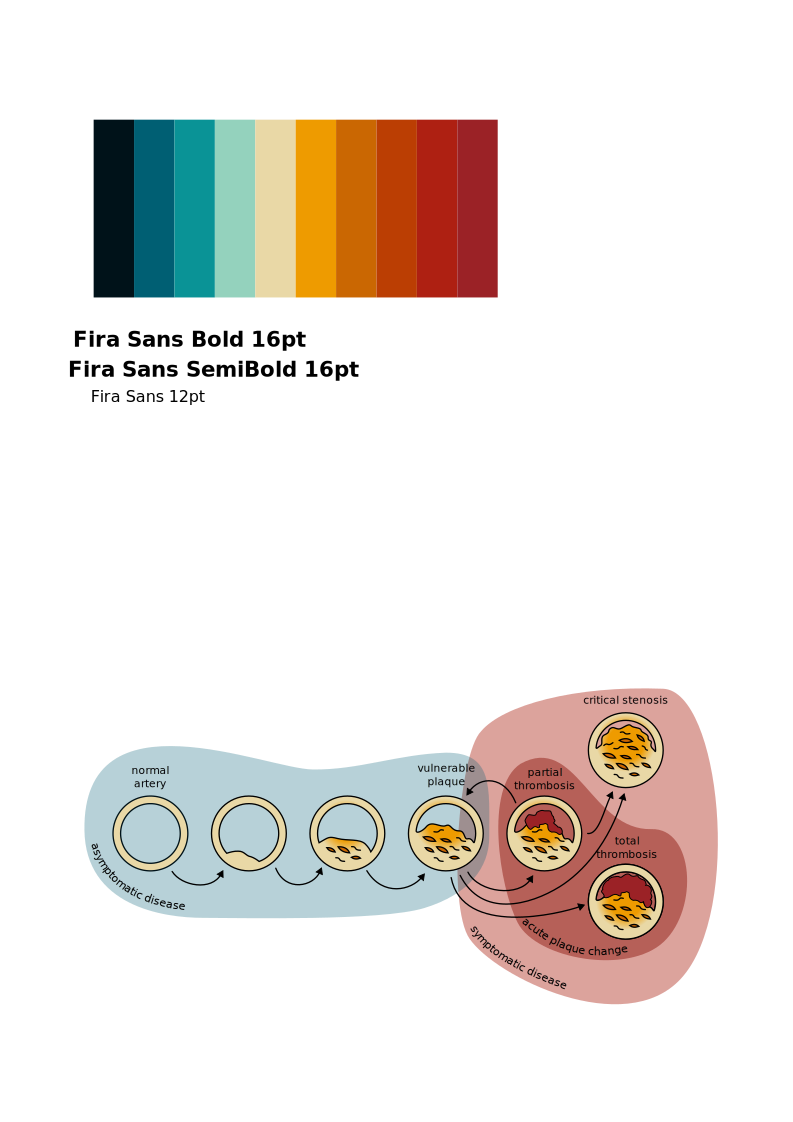
\includegraphics[width=\linewidth]{graphics/atherosclerosis}
    \caption[The process of atherosclerosis]{%
        The atherosclerotic process. 
        From a otherwise normal artery, 
        disruption of endothelial integrity and function, 
        through a combination of genetics and risk factors,
        leads to endothelial injury and low-grade inflammation. 
        Over time, this results in plaque formation through 
        accumulation of lipids, lipoproteins, calcium, and connective tissue.
        Eventually, the plaque may become \enquote{vulnerable}, 
        making it susceptible to sudden rupture or erosion. 
        Such an event can trigger thrombosis and acute changes in the plaque, 
        which, depending on their severity, may either immediately obstruct 
        the arterial lumen%
        ---leading to myocardial infarction or sudden cardiac death---%
        or contribute to further calcification through remodeling. 
        When the progressive narrowing of the arteries reaches a point where 
        it causes symptoms, the stenosis is considered critical, and the 
        myocardium experiences inadequate perfusion, manifesting as 
        ischemic heart disease.
    }
    \vspace{-5.1em}
    \label{fig:atherosclerosis}
\end{figurefw}
\vspace{9em}
% }}}

\section{Disease Manifestation}

The pathological process underlying ischemic heart disease 
is inherently chronic with atherosclerotic lesions 
gradually developing over time, 
but in the event of plaque rupture it can abruptly transition
and manifest as an acute condition.
The clinical presentation of ischemic heart disease  
is consequentially diverse and includes both acute 
~\autocite{byrne20232023}
and chronic coronary syndromes.
~\autocite{knuuti20192020}

Acute coronary syndromes includes 
\ac{UA}, \ac{STEMI}, and \ac{NSTEMI},
that collectively represents a spectrum of acute onset or progression of 
myocardial ischemia.
If the ischemia is sufficient to cause myocardial necrosis, 
it is per definition called \ac{MI}~\autocite{thygesenFourth2019}.
\ac{STEMI} and \ac{NSTEMI} are both forms of \ac{MI} that are distinguised
by a characteristic presence or absence of ST-segment elevation on a \ac{ECG}.
All of the acute coronary syndromes are typically associated 
with acute plaque change and atherothrombosis, 
and are medical emergencies that require immediate 
intervention to limit or prevent myocardial damage.
~\autocite{kumarRobbins2014}

% figure: ecg{{{
\begin{marginfigure}%
    \vspace{1em}
    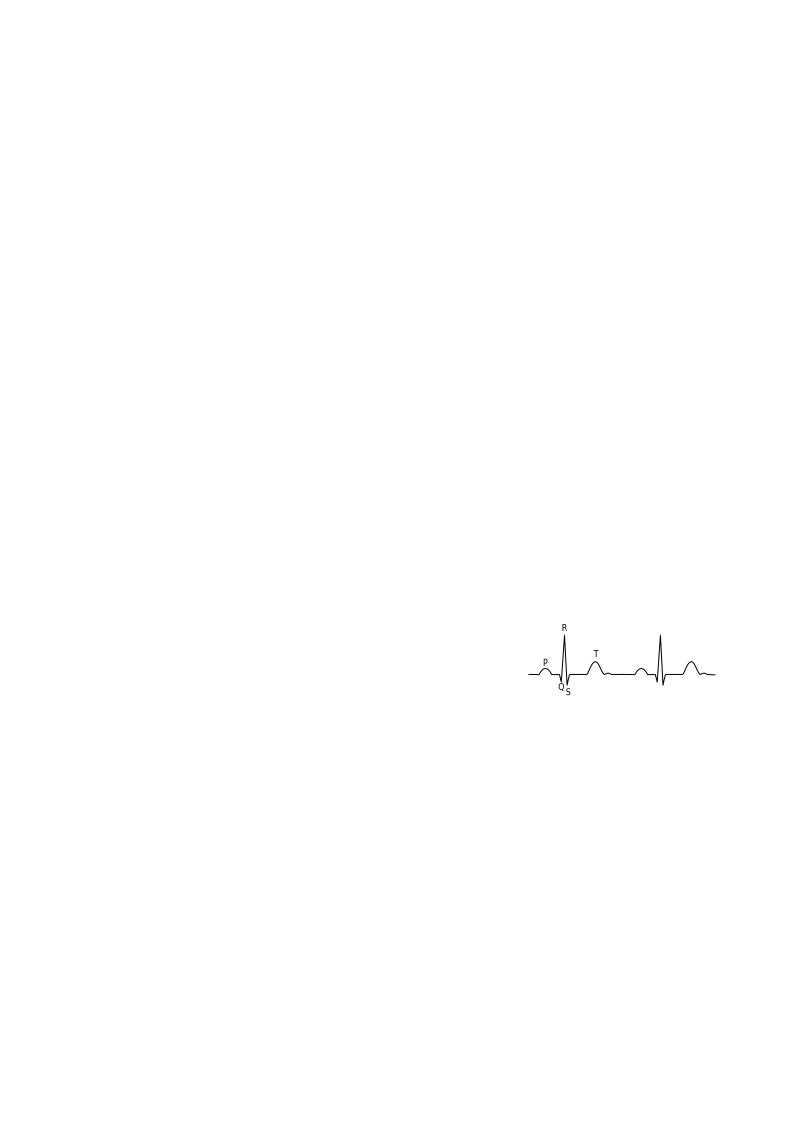
\includegraphics{graphics/electrocardiogram}
    \caption[Normal QRS complex]}}

Chronic coronary syndromes are more stable manifestations of the disease,
and include stable angina and chronic ischemic heart disease.
Stable angina, or \textit{angina pectoris}, is characterised by episodes of
crushing chest pain caused by myocardial ischemia, initially typically during
exercise.
By definition, the level of ischemia is not severe enough to lead to
tissue necrosis. 
~\autocite{knuuti20192020}
Unlike \ac{UA}, the symptoms of stable angina are often more predictable,
reliably triggered by a specific level of physical exertion, 
and typically absent when the individual is at rest. 
Chronic ischemic heart disease can either be a long-term progression of stable
ischemic heart disease or a late-stage stabilization following a \ac{MI} that
has undergone revascularization. 
~\autocite{knuuti20192020}
This condition represents the cumulative
effects of prolonged myocardial ischemia and accrued myocardial damage,
ultimately leading to progressive congestive heart failure.
~\autocite{kumarRobbins2014}

\section{Diagnosis and Treatment}

Since the 1950s, a series of groundbreaking scientific advances have improved 
our understanding and management of cardiovascular disease, leading to a 
drastic decline of mortality in ischemic heart disease.
~\autocite{nabelTale2012}
These advances span from from diagnostic imaging techniques to pharmacological
therapies and surgical interventions, each contributing to a more nuanced
understanding of the disease and more effective treatment options.
~\autocite{nabelTale2012}
To translate this constantly evolving body of knowledge into actionable medical
practice, the European Society of Cardiology (ESC) annually releases
comprehensive clinical practice guidelines that cover a wide array of
cardiovascular conditions.

In line with ESC guidelines, 
invasive management is the recommended approach
for immediate treatment of acute coronary syndromes.
This includes primary \ac{PCI}%
% sidenote: pci{{{
\sidenote[][-3em]{%
    \ac{PCI} is a minimally invasive procedure used for treatment of
    atherosclerosis. It involves the use of a small balloon catheter 
    to widen flow-limiting stenoses and restore cardiac perfusion.
} % }}}
for \ac{STEMI} and emergency angiography, 
potentially with concurrent \ac{PCI},
for patients with very high-risk \ac{NSTEMI} and \ac{UA}.
For those with a more stable presentation, but still at high-risk, 
angiography within the first 24 hours is indicated to
assess the need for revascularization. 
~\autocite{byrne20232023}
Based on factors such as the coronary anatomy, 
number and grade of stenotic vessels, 
and the estimated risk of surgical complications
\ac{CABG} is sometimes preferred over \ac{PCI}.
~\autocite{neumann20182019}
The primary objective of these interventions 
is providing timely revascularization where needed,
to restore coronary perfusion and limit myocardial damage.

Contrastingly, for chronic coronary syndromes,
invasive coronary angiography is typically not 
the first-line diagnostic test.
~\autocite{knuuti20192020}
However, for patients with a high clinical likelihood of ischemic heart
disease, who present with easily induceable or refractory angina pectoris 
and a high event risk, coronary angiography is recommended for assessment of
revascularization options.  
~\autocite{knuuti20192020}

Concurrent with invasive treatment, 
the guideline gives a class I recommendation for initiation 
of antithrombotic therapy in patients with \ac{IHD}. 
~\autocite{byrne20232023}
While the specifics of this therapy is beyond the scope of this thesis,
it generally involves a combination of antiplatelet medications, 
aimed at preventing further thrombotic events.
~\autocite{nabelTale2012}

\section{Secondary Prevention}

%% marginnote {{{
\marginnote[-2.5em]}}

Once the acute phase of the disease has been stabilized 
through revascularization or other treatments,
the clinical focus shifts to long-term management and secondary prevention.
Patients with established ischemic heart disease are generally of 
high risk of subsequent events, 
particularly if risk factors are not adequately managed.
~\autocite{clarkMetaAnalysis2005}
Guidelines advocate for a multifaceted approach to secondary prevention, 
incorporating lifestyle changes like quitting smoking and starting exercise, 
as well as pharmacological interventions such as lipid-lowering therapies. 
~\autocite{visseren20212021}

The goal of long-term treatment is essentially twofold:
to limit the progression of existing atherosclerotic plaque and 
to prevent and limit thrombus formation if plaques should rupture or erode.
~\autocite{foxMyth2020}
The clinical trajectories of patients with chronic manifestations of 
ischemic heart disease can remain stable for several years,
before unexpectedly deteriorating to 
major adverse cardiovascular events.
~\autocite{foxMyth2020}
Consequently, continuous monitoring and risk factor control 
are recommended to guide secondary prevention therapy.

In this setting,
risk stratification models that combine the clinical characteristics 
and risk factor profiles of the individual patient can be useful.
~\autocite{visseren20212021}
These models could help identify at-risk patients most likely to benefit from 
aggressive therapy. 
However, the real-world application of such models is not without challenges.
There is a need for rigorous validation studies to establish their 
clinical utility, as well as the development of 
protocols for their integration into routine clinical practice.

Additionally, there is a gap in understanding how comorbidities---%
whether cardiovascular or non-cardiovascular---%
affect outcomes and should be factored into treatment planning and prognosis.%
\sidenote[][13em]{\cite{visseren20212021}}
This is where the role of precision medicine becomes particularly salient. 
By leveraging advanced computational techniques and large-scale clinical data,
precision medicine has the potential to fill these gaps.

\section{Perspectives of Precision Medicine}

A 2013 Cochrane review on \citetitle{taylorStatins2013} concluded 
that statins effectively lower all-cause mortality and reduce the incidence
of both fatal and non-fatal cardiovascular events without any serious
adverse effects~\autocite{taylorStatins2013}.
For instance, the relative risk of fatal cardiovascular events 
when using statins as opposed to placebo
was estimated to \num{0.82} with a 
\si{95}{\%} \ac{CI} of \num{0.70} to \num{0.96}.
~\autocite{taylorStatins2013}
This suggests those treated with statins, on average,
are \si{18}{\%} less likely to die from cardiovascular causes. 
However, it is important to emphasize that this \si{18}{\%} 
reduction is an average effect for the \enquote{average individual}.
There might be groups of people for whom the reduction could be 
even higher, while others may see little to no benefit. 
Understanding and making use of such individual variability 
is the central objective of \enquote{precision medicine}.

Precision medicine is broadly speaking an approach to healthcare 
that aims to tailor medical treatment and management to the individual patient.
Instead of employing a \enquote{one-size-fits-all} methodology, 
where treatment and preventive care is being developed to the average patient,
precision medicine uses data-driven approaches to also account for 
the specific factors of the individual.
As such, the underlying idea of precision medicine is not really new;
tissue- and blood typing, for example,  
has been used to guide organ and blood donation for several decades.
However, the prospective of leveraging large clinical databases
and broad array of phenotypic information is adding renewed interest 
in the concept.
~\autocite{collinsNew2015}

% table: pgx-vars {{{
\begin{table*}[t]
\footnotesize
\centering
\tlfstyle
\begin{tabularx}{\linewidth}{r l p{3cm} X p{3.1cm}} 
\toprule
Gene & Variant & Drug & Description & Reference \\ 
\midrule

ABCG2 
& rs2231142
& rosuvastatin 
& Genotypes GT and TT is associated with increased plasma concentrations of 
rosuvastatin compared to genotype GG. 
&  \href{https://www.pharmgkb.org/clinicalAnnotation/1451666660}{1451666660}
\\

CYP2C9 
& *2 + *3 
& fluvastatin 
& Heterozygous or homozygous mutant allele carriers (*2 or *3) 
have an increased plasma concentration of fluvastatin.
& \href{https://www.pharmgkb.org/clinicalAnnotation/1451666740}{1451666740}
\\

CYP2C9 
& *2 + *3 
& fluvastatin 
& Heterozygous or homozygous mutant allele carriers (*2 or *3) 
have an increased likelihood of adverse events
when treated with fluvastatin compared to CYP2C9 *1/*1. 
&  \href{https://www.pharmgkb.org/clinicalAnnotation/1451678600}{1451678600}
\\

SLC01B1 
& rs4149056 
& rosuvastatin, simvastatin, pravastatin, lovastatin, fluvastatin, atorvastatin
& Genotypes CC and CT is associated with an increased risk of myopathy
when treated with either of the listed statins compared to genotype GG.
& \href{https://www.pharmgkb.org/clinicalAnnotation/1451357200}{1451357200},
\href{https://www.pharmgkb.org/clinicalAnnotation/1451244720}{1451244720},
\href{https://www.pharmgkb.org/clinicalAnnotation/1451244740}{1451244740},
\href{https://www.pharmgkb.org/clinicalAnnotation/1043880818}{1043880818},
\href{https://www.pharmgkb.org/clinicalAnnotation/655384011}{655384011},
\href{https://www.pharmgkb.org/clinicalAnnotation/1451465324}{1451465324}
\\

\bottomrule
\end{tabularx}
\caption[Pharmacogenomics of statins]{
	Examples of pharmacogenomics variants related to statin treatment 
	from the PharmGKB database.
	The included variants are all Level 1A clinical annotations, 
	which specify combinations of genetic variants and drugs for which there 
	is targeted prescribing guidance available either in
	current clinical guidelines or in FDA-approved drug labels. 
	Additionally, the Level 1A annotations are required to have a
	minimum of one supporting published article, in addition to the
	variant-specific recommendations.
 }
\label{tab:pgxvars}
\end{table*}% }}}

In the context of statin treatment,
this class of medication is generally both
highly effective and very well-tolerated, with limited side effects.
~\autocite{taylorStatins2013}
Some individuals may experience mild side effects such as muscle aches, 
while more severe side effects like myopathy or rhabdomyolysis 
are exceedingly rare.
~\autocite{thompsonStatinAssociated2003}
The underlying mechanism of 
statin-induced skeletal muscle side effects
is not well defined, 
but appears to be connected with the drug's serum concentration.
~\autocite{thompsonStatinAssociated2003}
Pharmacogenomics, a critical component of the pharmacological aspects of 
precision medicine, 
adds another layer to this understanding. 
It explores how genetic factors influence drug response, 
allowing for understanding etiology and more nuanced treatment plans. 
Genome-wide analyses have already identified \acp{SNP} 
that are associated with an increased risk 
of statin-induced side effects (Table \ref{tab:pgxvars}).
~\autocite{searchcollaborativegroupSLCO1B12008}
~\autocite{thornPharmGKB2013}
Through targeted screening of such genetic variants, 
and considering concurrent medication 
and experiential variability of the patients, 
it might be possible to refine medication regimens 
to maximize efficacy while minimizing side effects---%
a practical application of precision medicine.

Pharmacogenomics is an important step on the way,
but as such it is only one of the \enquote{building blocks} 
of precision medicine.
To fully realize the promise of precision medicine, 
we need a more holistic approach that consider not
only genetics but the multitude of other factors that 
can and will influence the ideal course of treatment.
Figure \ref{fig:precision-cardiology} shows a schematic of 
how such a precision cardiology workflow could look like.

% figure: precision cardiology {{{
\begin{figure}[bth]
    \vspace{1em}
    \caption[Schematic of Precision Cardiology]{%
    Schematic of a precision cardiology workflow.
    Patient characteristics encompass the full range of available data,
    including the individual's entire health and disease history.
    This information resides in an \ac{EHR} database, 
    which also holds data from other patients. 
    The \ac{EHR} database is a valuable research resource, 
    that can contribute to a curated clinical knowledge base. 
    Patient data, the \ac{EHR} database, 
    and the knowledge base is used as input 
    by computational algorithms and tools. 
    These tools act as clinical decision support systems, 
    providing prognostic and diagnostic models. 
    The outputs of these models 
    are shared with both the patient and the physician, 
    facilitating personalized treatment 
    through shared decision-making.%
    }
	\includegraphics{graphics/precision-cardiology}
    \label{fig:precision-cardiology}
    \setfloatalignment{t}
    \vspace{-3em}
\end{figure}
% }}}

The central elements of this precision cardiology workflow is:
\begin{enumerate*}
    \item big data collection and organization
    \item computer-based clinical tools and algorithms
    \item implementation of these tools in clinical decision making
\end{enumerate*}.
In the research underlying this thesis, 
the primary emphasis have been on (i) and (ii),
but without (iii) the advances of precision medicine
will remain mostly academic in scope.
The challenges and future perspectives of the clinical implementation
will be discussed later in the thesis.
Focusing on the first two elements, 
how do we derive tools and algorithms from big datasets?

       
\chapter{Fundamentals of Machine Learning and Neural Networks}
\label{ml-fundamentals}

In modern medicine, 
ever increasing amounts of data 
is continuously being generated and collected.
Ranging from structured administrative data 
used primarily for billing purposes
to advanced imaging and high-througput \enquote{omics} analyses,
the array of available data is as diverse as it is plentiful.
Making sense and making use of such massive amounts of data 
necessitates automated methods for data analysis.

% figure: hierarchy of artificial intelligence {{{
\begin{marginfigure}[3em]
    \centering
	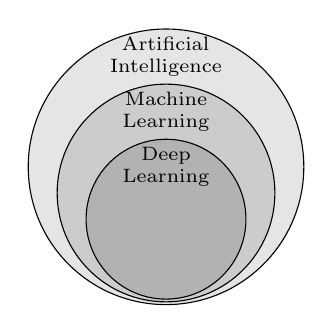
\begin{tikzpicture}[scale=1.75]
        \draw[black, fill=black!10] (0,  0.00) circle (1.00);
        \draw[black, fill=black!20] (0, -0.19) circle (0.79);
        \draw[black, fill=black!30] (0, -0.38) circle (0.58);
        \node[font=\scriptsize, text width=1.8cm, align=center] 
            at (0, 0.8) {Artificial Intelligence};
        \node[font=\scriptsize, text width=1.8cm, align=center] 
            at (0, 0.4) {Machine Learning};
        \node[font=\scriptsize, text width=1.4cm, align=center] 
            at (0, 0.0) {Deep Learning};
	\end{tikzpicture}
    \caption[The hierarchy of artificial intelligence (AI)]{%
        \Ac*{AI} is an umbrella term for computer software 
        that have some sort of \enquote{intelligence} and
        \ac*{ML} is a collection of methods through which 
        that can be achieved. 
        \Ac*{DL}, a specific method in \acs*{ML}, 
        relies on neural networks with many layers
        to analyse complex data.
    }
    \label{fig:artificial-intelligence}
\end{marginfigure}% }}}

\Ac{AI}, and specificically \ac{ML} (\cref{fig:artificial-intelligence}),
seeks to address this need by development of methods and algorithms
that allows computers to \enquote{learn} from data to solve new problems
instead of them being explicitly programmed.
~\autocite{goodfellow2016deep}
The field of \ac{ML} have progressed exponentially
over the past couple of decades, 
and with the advent of generative \ac{AI} models like 
GPT-4~\autocite{openaiGPT42023} and
DALL-E~\autocite{rameshZeroShot2021}
there is a growing public interest in the use of \ac{AI} and \ac{ML}.
In the context of precision medicine,
the promise of \ac{AI} lies in the ability 
to integrate large amounts of data from huge data sets
and register and highlight patterns with clinical importance.
In his review on artificial intelligence in medicine%
\autocite{topolHighperformance2019}, 
Eric Topol expresses his view, that in the not so distant future
\blockquote{%
almost every type of clinician, ranging from specialty doctor to paramedic,
will be using AI technology, and in particular deep learning}.

The underlying principle of \ac{ML} is to formulate a learning problem with a
well-defined objective and a quantifiable measure of performance.
~\autocite{murphyMachine2012}
Subsequently,
a loosely defined computer program is established and fed with data
representing said objective.
Guided by the performance metric, \ac{ML}
algorithms iteratively refine the underlying computer program until the
objective is optimally addressed. 
In his 1997 book \citetitle{mitchellMachine1997},
\citeauthor*{mitchellMachine1997} defines this formally as:
\begin{displayquote}[mitchellMachine1997]
   A computer program is said to learn from experience \(E\)
   with respect to some class of tasks \(T\) and performance measure \(P\),
   if its performance at tasks in \(T\), as measured by \(P\), 
   improves with experience \(E\).
\end{displayquote}
Though this conceptual framework is common to all \ac{ML} models, 
the diversity in \ac{ML} arises from not only the specific \ac{ML} algorithm, 
but also choices regarding objectives, performance metrics, and program attributes. 
These selections introduce the myriad variations and nuances within \ac{ML}, 
which can be broadly categorized into two distinct approaches:
supervised learning
and 
unsupervised learning.
~\autocite{murphyMachine2012}

\section{Supervised Learning}

In supervised learning, models are trained on labeled examples---%
a dataset 
\(\mathfrak{D} = \{(\vec{x}_i, y_i) \mid i \in \{1, \ldots, N\}\} \) 
of size \(N\) that contains both input features \(\vec{x}\)
and corresponding correct output values \(y\)
for all the examples in the dataset. 
Here \( \mathfrak{D} \) is typically refered to as the training set.
~\autocite{murphyMachine2012}
The primary aim in supervised learning 
is to learn a function \(f\) that correctly 
maps input data \(\vec{x}\) to output data \(y\), 
i.e. correctly assigns output labels or values
based on the features present in the input data.
When the output is discrete labels or classes, 
the task is called a classification problem.
Conversely, 
if the output is continuous values,
it is called a regression problem.

Illustrating with a supervised learning task in the domain of classification, 
we can consider a database of coronary angiography images that have been 
manually annotated to indicate the presence or absence of critical stenosis 
in any of the coronary arteries. 
In this scenario, 
the output classes are denoted as 
\(y \in \{\textsf{stenosis}, \textsf{no stenosis}\}\), 
and the objective is to classify the images 
into either of these categories based on their pixel values.
The labeled data is being used to guide and \enquote{supervise}
the model in order for it accurately accomplish this categorisation.

Two other examples of supervised learning tasks is presented in 
\nameref{chap:paper-2} and 
\nameref{chap:paper-3}
within this thesis.
However, these tasks differ from classical supervised learning
in that they involve time-to-event predictions and censored labels.
This subject matter will be elaborated upon in the next chapter:
\nameref{survival-analysis}.

\section{Unsupervised Learning}

In contrast to supervised learning,
unsupervised learning is concerned with finding 
underlying patterns or structures within unlabeled datasets. 
In this paradigm, the algorithm operates without the aid of 
predetermined labels or categories, instead learning from the data itself. 
The aim is to discover intrinsic structure in the dataset, 
which can then be used for tasks such as 
dimensionality reduction, clustering, or anomaly detection.
\sidecite[-8em]{murphyMachine2012}

A canonical example of unsupervised learning is the problem of clustering,
where the objective is to partition a set of objects into subgroups based
on similarity.
\sidecite[-11em]{murphyMachine2012}
Things that are similar should be grouped together and
should be relatively dissimilar to things in other groups.
Defining what constitutes \enquote{similar} 
is therefore a central challenge in clustering;
different measures of similarity often result
in fundamentally different clusterings.%
% card clustering analogy{{{
\sidenote[][-15em]{%
    To illustrate, we can consider a set of playing cards,
    that for convenience is limited to aces, court cards, and tens. 
    One possible clustering groups the cards by suit:
\begin{equation*}
    \begin{array}{@{}c@{}ccccc}
    \{
    &\{ 10\twemoji{heart suit}, 
    &    J\twemoji{heart suit}, 
    &    Q\twemoji{heart suit}, 
    &    K\twemoji{heart suit}, 
    &    A\twemoji{heart suit}
    \}, \\
    &\{ 10\twemoji{spade suit}, 
    &    J\twemoji{spade suit}, 
    &    Q\twemoji{spade suit}, 
    &    K\twemoji{spade suit}, 
    &    A\twemoji{spade suit}
    \}, \\
    &\{ 10\twemoji{diamond suit}, 
    &    J\twemoji{diamond suit}, 
    &    Q\twemoji{diamond suit}, 
    &    K\twemoji{diamond suit}, 
    &    A\twemoji{diamond suit}
    \}, \\
    &\{ 10\twemoji{club suit}, 
    &    J\twemoji{club suit}, 
    &    Q\twemoji{club suit}, 
    &    K\twemoji{club suit}, 
    &    A\twemoji{club suit}
    \}\}
\end{array}
\end{equation*}
Another equally valid clustering groups them by rank:
\begin{equation*}
    \begin{array}{@{}c@{}cccc}
\{ 
   &\{10\twemoji{heart suit},
   & 10\twemoji{spade suit}, 
   & 10\twemoji{diamond suit}, 
   & 10\twemoji{club suit}
\}, \\
   &\{J\twemoji{heart suit}, 
   &  J\twemoji{spade suit}, 
   &  J\twemoji{diamond suit}, 
   &  J\twemoji{club suit}
\}, \\
   &\{Q\twemoji{heart suit}, 
   &  Q\twemoji{spade suit}, 
   &  Q\twemoji{diamond suit}, 
   &  Q\twemoji{club suit}
\}, \\
   &\{K\twemoji{heart suit},
   &  K\twemoji{spade suit},
   &  K\twemoji{diamond suit},
   &  K\twemoji{club suit}
\}, \\
   &\{A\twemoji{heart suit},
   &  A\twemoji{spade suit}, 
   &  A\twemoji{diamond suit}, 
   &  A\twemoji{club suit}
\}\}
\end{array}
\end{equation*}
The choice between these clusterings depends on whether
suits or ranks are considered more important,
which probably depends on the specific card game in question.
This challenge applies to most clustering problems---%
the ideal clustering is usually highly context dependent.
}
% }}}
Clustering lies at the heart of precision medicine:
By identifying distinct subgroups of patients with varying risk profiles, 
clinicians can tailor prevention and treatment strategies more effectively, 
optimizing healthcare outcomes as a result.

In \nameref{chap:paper-1} of this thesis,
we present an example of clustering analysis of patients with 
ischemic heart disease by considering the patterns of comorbidity 
common in subgroups of patients.
The specific methods used in this work is outlined 
in the chapter \nameref{chap:outline-paper-1}.

\section{Generalization and Overfitting}
\label{overfitting}

% figure: generalization error {{{
\begin{marginfigure}[3em]
    \centering
	\includegraphics{graphics/overfitting-2}
    \caption[Overfitting as Function of Number of Epochs]{%
        Training a neural network model for many iterations 
        runs the risk of overfitting the model to the training data.
        Although the training error keeps decreasing, 
        it happens at the expense of increased generalization error.
        Inspired by \cite{goodfellow2016deep}.
    }
    \label{fig:generalization-error}
\end{marginfigure}
% }}}

Returning to supervised learning,
it is important to note that achieving good performance on the 
training set is not the sole objective.
For a \ac{ML} model to be of utility, 
it should maintain its accuracy
when applied to unseen data.
This concept is known as \textit{generalization} and
is a central problem in supervised learning---%
especially when dealing with highly flexible models 
such as neural networks.
~\autocite{goodfellow2016deep}
We can keep track of a model's generalization error 
by introducing an additional dataset, 
that is kept separate from the training set. 
This additional set of labeled examples is refered to as the test set
and is exclusively used for evaluation of model performance.
Assuming that the test set is representative%
\sidenote{%{{{
    An underlying assumption is that the two datasets are 
    independent and identically distributed 
    (typically abbreviated as i.i.d.),
    and thus share the same underlying \textit{data-generating process}.
    [\cite{goodfellow2016deep}]
},
% }}}
the performance on the test set can be used as an estimate of 
the generalization error since it represents unseen data.


\Cref{fig:generalization-error} shows a theoretical training history 
of a neural network model where the performance is calculated 
on both a training and a test set after each iteration of the training.
Here it is illustrated that 
the training loss is monotonically decreasing 
with increasing number of iterations.
The validation loss is at first also decreasing,
but if training continues for long enough,
at some point it will start to increase instead.
The divergence between training and test set performance 
indicates overfitting:
instead of learning generalizable patterns representative of the underlying 
data-generating process,
the model starts to learn or even memorise
the noise and idiosyncracies of the data that,
although characteristic in the narrow scope of the training set,
would not be representative of neither biology nor disease etiology.
~\autocite{murphyMachine2012}
As a consequence, the test set performance is considerably worse 
than the training set performance.

% figure: overfitting {{{
\begin{figure}[htb]
	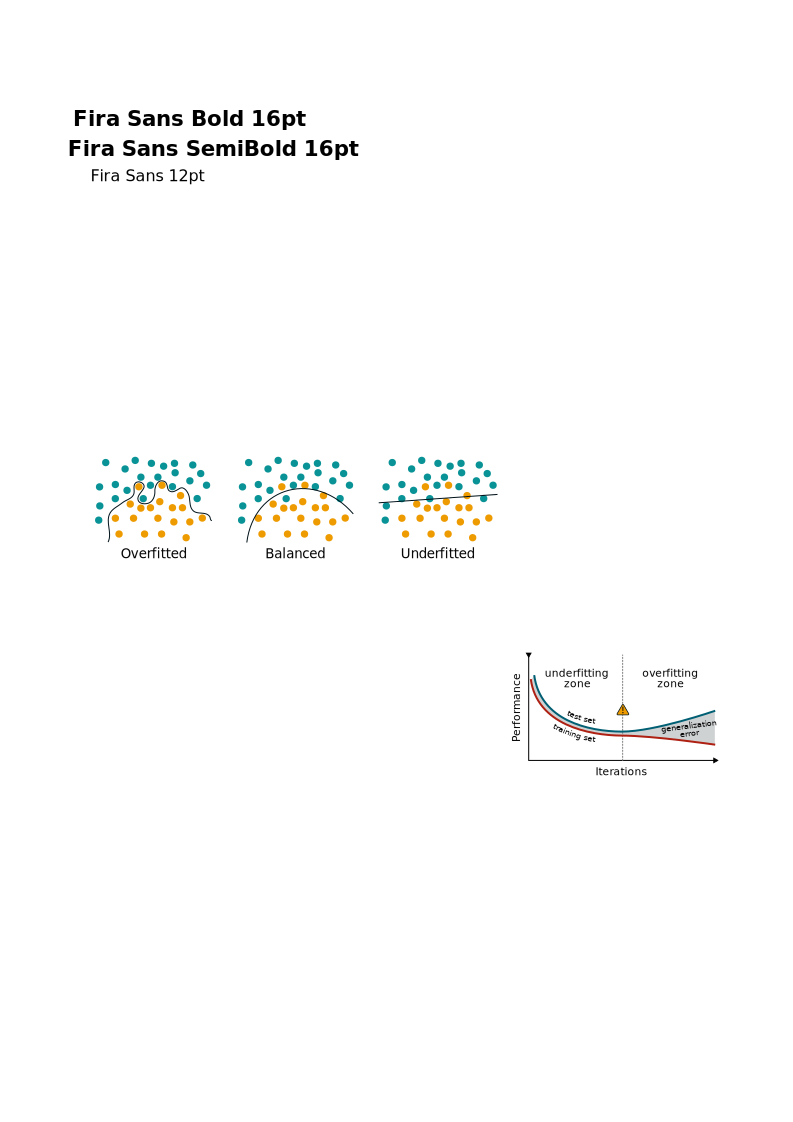
\includegraphics{graphics/overfitting}
    \setfloatalignment{t}
    \caption[What is Overfitting?][-1em]{%
        Illustration of overfitting and underfitting 
        in a simple classification task.
        An overfitted model learns the training data too well,
        and may even remember noise and outliers,
        which makes it perform poorly on unseen data.
        Underfitted models, on the other hand,
        are to simple to capture meaningful patterns in the data.
    }
    \label{fig:overfitting}
    \vspace{-2em}
\end{figure}
% }}}

Overfitting, and its counterpart, underfitting,
are key considerations in training of \ac{ML} models (\cref{fig:overfitting}).
Overfitting happens 
when a model learns the details of the training data too well, 
including the noise, 
which makes it perform poorly on unseen data.
In constrast,
underfitting occurs when the model is too simplistic 
to capture meaningful patterns in the data, 
resulting in poor performance on both the training and test sets.
Both issues highlight the need for balancing the complexity of models,
to ensure that they can effectively generalize to unobserved data.
In the section \nameref{sec:regularization},
I will outline some of the specific methods 
used to balance the complexity 
of neural network models.

\clearpage
\section{Neural Networks}

% figure: neuron{{{
\begin{marginfigure}[3em]
	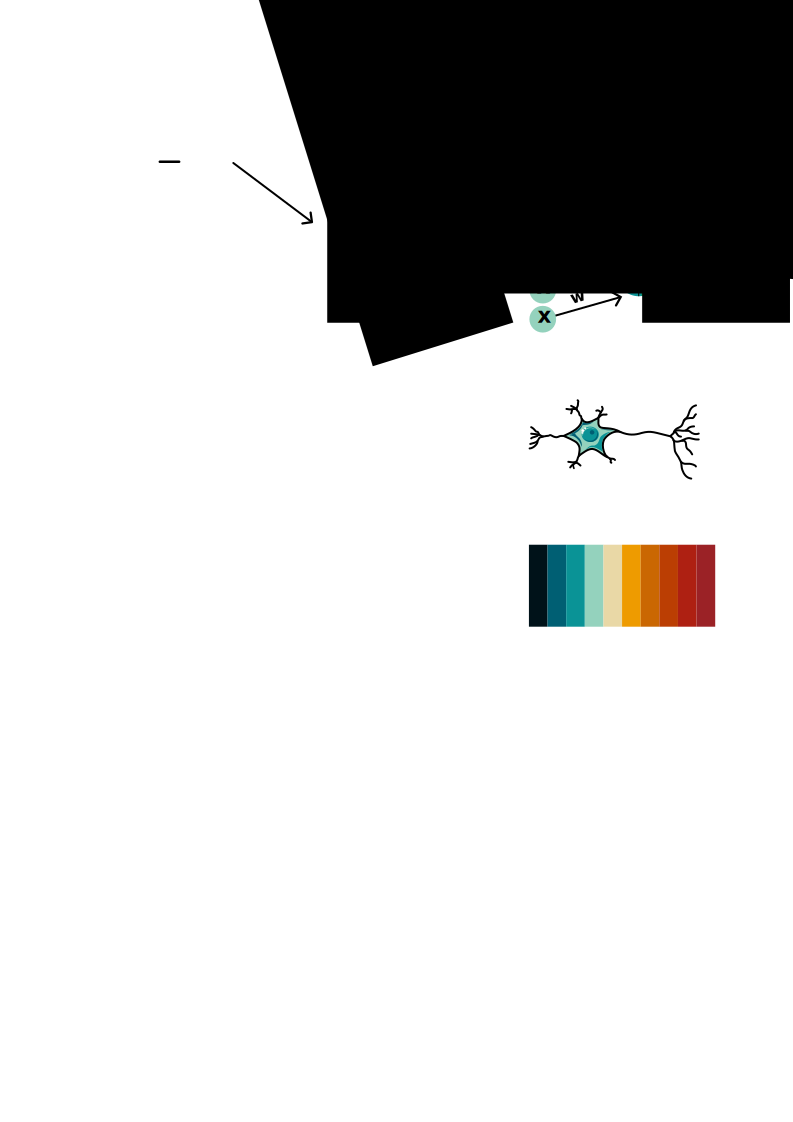
\includegraphics[width=\linewidth]{graphics/neuron}
    \caption[Schematic diagram of a neuron]{%
        Schematic diagram of a neuron.
        A typical neuron has a dendrites, a cell body, and a single axon; 
        the dendrites receive input signals from other neurons,
        and propagates output signals along the axon.
    }
    \label{fig:neuron}
\end{marginfigure}% }}}

In \nameref{chap:paper-2} and \nameref{chap:paper-3}, 
neural network models are utilized to 
develop risk prediction models for ischemic heart disease.
Neural networks is a versatile class of machine learning models
well-suited for handling large and heterogeneous datasets, 
and they currently represent the state-of-the-art in \ac{ML}.
The rest of this chapter will concentrate mainly on neural networks, 
outlining the methodological details and highlight 
relevant practical challenges and considerations 
in their implementation.

Historically, neural networks were designed
using the archicteture of neurons in a human brain as inspiration.
~\autocite{goodfellow2016deep}
The simplest model is that of a perceptron, 
which can be seen as a computational approximation
of a real neuron or nerve cell.
~\autocite{charniakIntroduction2019}
A typical neuron has many dendrites, a cell body, and a single axon 
(\cref{fig:neuron}).
The dendrites carries the input signal to a neuron,
and if the cumulative signal is great enough%
\sidenote[][]{
    This threshold is known as 
    the \textit{threshold potential},
    and is typically between -50 and -55 mV.
}, 
then the neuron will propagate an action potential down the axon%
\autocite{seifterConcepts2005}.
In similar fashion, a perceptron receives may receive many different inputs
and produces a single output (\cref{fig:perceptron}).
In the case of a neuron, the \enquote{all-or-none} principle means
that nerve cells either signals at full strength or not all.
For a perceptron, this principle can be emulated
with the followingly Heaviside step function:
~\autocite{charniakIntroduction2019}

\begin{equation}
    \label{eq:step-function}
    g_{\phi}(\vec{x})  = 
        \begin{cases}
            1 & \text{if } b + \vec{w} \cdot \vec{x} > 0\\
            0 & \text{otherwise}
        \end{cases}
\end{equation}

% figure: perceptron{{{
\begin{marginfigure}%
	\includegraphics[width=\linewidth]{graphics/perceptron}
	\caption{Schematic diagram of a perceptron}
    \label{fig:perceptron}
\end{marginfigure}% }}}

By combing several of such artificial neurons,
in a multilayer-perceptron or feedforward neural network,
we can create a model that, in theory,
can learn even the most complex of patterns.
~\autocite{bishopNeural1995}
In this design (\cref{fig:nn-structure}),
information travels in one direction, from the input layer
through the hidden layers, and finally to the output layer. 
Each layer in a feedforward neural network is
fully connected to the subsequent layer---%
every neuron in one layer is connected to every neuron in the next.

% figure: neural-network {{{
\begin{figure}[tb]
\tikzstyle{node}        =[thick, circle, draw=color0, minimum size=23, 
                          inner sep=0.5, outer sep=0.6]
\tikzstyle{node in}     =[node, fill=color2]
\tikzstyle{node hidden} =[node, fill=color3]
\tikzstyle{node out}    =[node, fill=color4]
\tikzstyle{connect}     =[thick, color0]
\tikzstyle{label}       =[above=0, align=center, font=\sffamily]
\tikzset{ % node styles,
  node 1/.style={node in},
  node 2/.style={node hidden},
  node 3/.style={node out},
}
\def\nstyle{int(\lay<\Nnodlen?min(2,\lay):3)} % map layer number onto 1, 2, or 3
\centering
\begin{tikzpicture}[x=2.0cm, y=1.0cm]
  \readlist\Nnod{6,4,4,4,5}
  \foreachitem \N \in \Nnod{ % loop over layers
    \def\lay{\Ncnt}  % alias of index of current layer
    \pgfmathsetmacro\prev{int(\Ncnt-1)} % number of previous layer
    \foreach \i [evaluate={\y=\N/2-\i; \x=\lay; \n=\nstyle;}] in {1,...,\N}{
      % nodes
      \node[node \n] (N\lay-\i) at (\x,\y) {};
      % connections
      \ifnum\lay>1
        \foreach \j in {1,...,\Nnod[\prev]}{
          \draw[connect, white, line width=1.2] (N\prev-\j) -- (N\lay-\i);
          \draw[connect] (N\prev-\j) -- (N\lay-\i);
        }
      \fi 
    }
  }
  % labels
  \node[label] at (N1-1.90) { Input };
  \node[label] at (N3-1.90) { Hidden Layers };
  \node[label] at (N5-1.90) { Output };
\end{tikzpicture}
\caption[Schematic of a Feedforward Neural Network]{
    A schematic representation of a feedforward neural network, 
    comprising an input layer, multiple hidden layers, and an output layer. 
    Each circle denotes a neuron, and the connecting lines represent 
    connections between neurons.}
\label{fig:nn-structure}
\end{figure}
% }}}

In the context of modern neural networks, 
the simplistic step function in \cref{eq:step-function} 
has certain limitations.
In particular, it is non-differentiable at \(x = 0\) and
has a zero derivative elsewhere, 
rendering it incompatible with gradient-based optimization algorithms.  
To address these issues, other activation functions
have been introduced,
with the sigmoid, \ac{tanh}, and \ac{ReLU} being popular choices 
(\cref{fig:act-fn}), but many other variations exists.
~\autocite{cholletDeep2021}

% figure: activation functions {{{
\begin{figure}[htb]
\pgfplotsset{%
    every axis/.append style={%
        tick label style={/pgf/number format/fixed},
        font=\footnotesize,
        ylabel near ticks,
        xlabel near ticks,
        grid=major
    }}
\centering
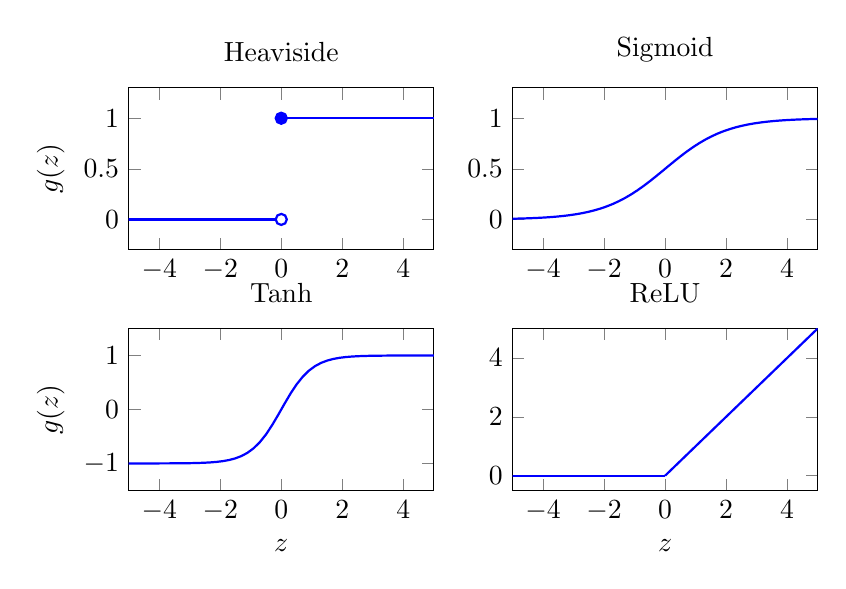
\begin{tikzpicture}% {{{
    \begin{groupplot}[%
        group style={group size= 2 by 2}, 
        width=0.45\linewidth, height=0.30\linewidth
    ]
    \nextgroupplot[
            title=Heaviside, 
            ylabel= \(g(z)\),
            xmin=-5, xmax=5,
            ymin=-0.30, ymax=1.30
        ]
        \addplot[mark=*, blue, thick, samples at={-5.1, 0},
            mark options={fill=white}]  {0};
        \addplot[mark=*, blue, thick, samples at={0, 5.1},
            mark options={}]  {1};
    %% 
    \nextgroupplot[
            title=Sigmoid, 
            xmin=-5, xmax=5,
            ymin=-0.30, ymax=1.30
        ]
        \addplot[domain=-10:10, blue, thick, samples=100] {1/(1+exp(-x))};
    %% 
    \nextgroupplot[
            title=Tanh, 
            ylabel= \(g(z)\),
            xlabel= \(z\),
            xmin=-5, xmax=5,
            ymin=-1.5, ymax=1.5
        ]
        \addplot[domain=-10:10, blue, thick, samples=100] {tanh(x)};
    \nextgroupplot[
            title=ReLU, 
            xlabel= \(z\),
            xmin=-5, xmax=5,
            ymin=-0.5, ymax=5
        ]
        \addplot[domain=-10:0, blue, thick] {0};
        \addplot[domain=0:10,  blue, thick] {x};
        
    \end{groupplot}
\end{tikzpicture}% }}}
\caption[Well-known Activation Functions]{%
    Plots of well-known activation functions used in neural networks. 
    From top left to bottom right: 
    The Heaviside step function, 
    the sigmoid (or logistic) function,
    the \acf{tanh}, and the \acf{ReLU}.
    Each function is plotted against its input value \(z\) 
    to show its respective output \(g(z)\).}
\label{fig:act-fn}
\end{figure}% }}}

In addition to feed forward neural networks, 
ongoing research have developed other neural network architectures 
tailored to particular types of data. 
For example, convolutional neural networks were designed 
for processing image data
~\autocite{lecunHandwritten1989}
and have revolutionized the field of
computer vision.
~\autocite{prince2023understanding}
Similarly, recurrent neural networks,
such as the long short-term memory nework,
can model sequential data
and have had great impact for both time series analysis 
and natural language processing.
~\autocite{hochreiterLong1997}
Another innovation, 
is the introduction of skip or residual connections 
in architectures such as residual networks (ResNet),
which have enabled the training of exceptionally deep networks.
~\autocite{heDeep2015}

\clearpage

\section{Practical Implementation of Neural Networks}

In developing neural network models for \ac{ML} objectives,
several methodological considerations and decisions 
have to be made.
It is not feasible to exhaustively cover
every nuance within the scope of this thesis, 
instead the book \citetitle{goodfellow2016deep} 
serves as a comprehensive reference.%
~\sidecite[-3em]{goodfellow2016deep}
As a guide, 
the following list provides a high-level overview of the typical workflow:%
\sidenote[][-4em]{%{{{
    The list draws inspiration from chapter 19.9 in 
    \cite{russellArtificial2009} and chapter 4 in
    \cite{cholletDeep2021}.
}% }}}

\begin{fullwidth}
%\setcounter{unbalance}{3}
\begin{multicols}{2}
\raggedcolumns
\begin{enumerate}
    \item \label{itm:problem}
        \textit{Problem Definition:} 
        Clearly describe the problem, 
        and in the process identify if the objective belongs to 
        classification, regression, or a third category.
        Attached to the objective should be a measure of performance, 
        which in the neural network literature typically is known as 
        loss function, which is used to direct training.

    \item \textit{Preparing the Data}:

        \begin{enumerate}
        \item \label{itm:data-collection}
            \textit{Data Collection:} 
            Gather and organize data for both training and testing the model.
            Importantly, data should be of reasonable quality,
            pertinent to the problem at hand, and of sufficient quantity.
            If not, it can be a good idea to adjust \cref{itm:problem} 
            to better reflect the available data.

        \item \label{itm:data-preprocessing}
            \textit{Data Preprocessing:} 
            Prepare the data for model training, 
            which may include cleaning, normalization, and transformation tasks.
            The classical saying \enquote{garbage in, garbage out}
            is worth repeating here.
            Any data-informed tasks (e.g. normalization) should exclusively
            be setup using the training set to avoid leakage of data.
            \unskip\footnotemark
        \end{enumerate}

    \item \label{itm:model-specification}
        \textit{Network Structure:} 
        Choose the architecture of the neural network, 
        defining elements such as the number of layers, 
        number of neurons within each layer, 
        and activation functions.
        Certain architectures have shown to be useful for specific 
        types of data, e.g. convolutional neural networks are
        typically the architecture of choice for computer vision tasks.%
        \unskip\footnotemark
        
    \columnbreak
    \item \label{itm:training-specification}
        \textit{Configuring Model Training:}
        \begin{enumerate}%
        \item \label{itm:optimizer}
            \textit{Optimization Algorithm:} 
            Choose and configure an optimization algorithm.
            \Ac{SGD} and variants thereof 
            are the most common algorithms for neural networks,
            \unskip\footnotemark
            and all have different 
            parameters that needs to be defined and possibly tuned 
            (see \cref{itm:hyperparameter}), 
            such as e.g. the learning rate.

        \item \label{itm:regularization}
            \textit{Regularization:} 
            To mitigate overfitting and ensure better generalization,
            consider using regularization techniques such as 
            L1/L2-regularization or Dropout.
            \unskip\footnotemark
        \end{enumerate}

    \item \label{itm:hyperparameter}
        \textit{Hyperparameter Tuning:} 
        Tweak and adjust the relevant hyperparameters specified
        in any of the previous steps,
        including learning rate (from \cref{itm:optimizer})
        and specific details of the neural network architecture 
        (\cref{itm:model-specification})
        to find the best configuration.
        This typically involves training many different intermediate
        versions of the model and evaluating their performance
        using a validation set.

    \item \label{itm:training}
        \textit{Model Training:} 
        Train the final version of the model 
        using the designated training set.

    \item \label{itm:evaluation}
        \textit{Model Evaluation:} 
        Assess the trained model using the test set, 
        calculating metrics like accuracy, precision, and recall 
        to gauge its effectiveness.
        Model explainability techniques can here 
        be helpful in aiding the interpretation of the model.
\end{enumerate}
\end{multicols}
\end{fullwidth}

\footnotetext{\cite{cholletDeep2021}}
\footcitetext{lecunHandwritten1989}
\footcitetext{cholletDeep2021}
\footcitetext{goodfellow2016deep}

While presented as sequential steps, 
the items in the list are almost all interrelated 
and can and should affect one another. 
As an example, 
it especially evident that
\cref{itm:data-collection} 
drastically influences the range of possibilities in 
\cref{itm:problem}.
In the remaining sections of this chapter, 
I will be highlighting select concepts integral to  
building neural network models which have specific
relevance to the papers included in the thesis.

\section{Model Selection}
\label{sec:model-selection}

We can estimate the generalization error of a model
by evaluating it on a test set.
If we are only creating a single model,
then this approach suffices. 
However, we might want to compare many different models,
or slightly tweak an already existing model,
such that we can select the best performing version.
This is particularly relevant in the context of hyperparameter optimization,
a topic that I will return to later in this chapter.
If we select the final model based on the test set alone,
we might inadvertently have biased the process,
and could, in a sense, have overfitted to the test data.
~\autocite{murphyMachine2012}
To avoid this, we need to completely hide away the test data
until we are done with training, experimenting, 
and model selection.
To enable this, a common solution is to introduce a third dataset by splitting 
the training data into two sets of data: a training set and a validation set.
The three sets of data used in the development process is then: 
%
\begin{itemize}
    \item a training set to train or develop candidate models
    \item a validation set to evaluate and select the best model
    \item a test set for the final evaluation of model performance
\end{itemize}

\section{Regularization}
\label{sec:regularization}

Regularization is a collection of strategies used to avoid
overfitting by penalizing the complexity of \ac{ML} models.
Two classical examples are L2 and L1 regularization
that adds an regularization term \(\omega\),
on the model parameters \(\phi\),
to the loss function \(\mathcal{L}\).
~\autocite{goodfellow2016deep}

\vspace{1.5em}
\begin{equation}
    \widetilde{\mathcal{L}} (\vec{\phi} , \mathsf{X}, \vec{y}) =
    \mathcal{L} (\vec{\phi} , \mathsf{X}, \vec{y}) +
    \eqnmarkbox[blue]{node1}{ \omega (\vec{\phi})}
\end{equation}
\annotate[yshift=.5em]{left}{node1}{regularization term}

In the case of L1 regularization, 
the regularization term consists of 
the sum of the absolute values of the model parameters, 
also known as the L1 norm. 
For L2 regularization, 
the term comprises the sum of the squares of the model parameters, 
otherwise known as the squared L2 norm.
~\autocite{murphyMachine2012}
%
\begin{alignat}{3}
    &L1: \quad \omega (\vec{\phi}) 
        &&= \lambda||\vec{\phi}||_1 
        &&= \lambda\sum_{i}|\phi_i|  \\
    &L2: \quad \omega (\vec{\phi}) 
        &&= \lambda||\vec{\phi}||_2^2 
        &&= \lambda\sum_{i} \phi_i^2
\end{alignat}

The regularization strength is controlled by a hyperparameter, \(\lambda\);
a value close to zero imposes minimal regularization, 
while larger values increases the amount.
In the context of neural networks, 
another commonly used regularization method is \textit{dropout}.
~\autocite{srivastava2014dropout}
This method simply involves randomly dropping some of the output features
of the hidden layers during each iteration of the training.
This process in a sense creates a different architecture at every step, discouraging the model from becoming overly dependent on any single feature 
and thereby enhances generalization. 
~\autocite{charniakIntroduction2019}
Empirically, dropout have been found to give significant improvements across
many different architectures 
~\autocite{srivastava2014dropout}
and is a consequence broadly utilized.
~\autocite{charniakIntroduction2019}
The droput rate, which controls the probability \(p\) of dropping out each
individual unit, is a hyperparameter that needs to be specified.

\section{Hyperparameter Optimization}

Neural networks, as well as most other \ac{ML} models,
have parameters and settings that are not adjusted 
during training and therefore needs to pre-specified.
~\autocite{goodfellow2016deep}
These parameters are known as hyperparameters, 
and common examples include aspects such as 
learning rate,
number of layers in the neural network,
number of nodes in each layer,
Other specific examples have also been described previously in this chapter.

Although it is possible to assign default values to hyperparameters 
based on prior experience and personal preference, 
it is imperative to acknowledge their possible impact on model performance.
Consequently, it is common to explore different setting and combinations
of hyperparameters in the model building process.
~\autocite{goodfellow2016deep}
In the field of machine learning, this process is known as \ac{HPO}.

If the number of hyperparameters are sufficiently small,
a commonly employed strategy for \ac{HPO} 
is creating a range of possible candidate values 
for each hyperparameter and 
simply testing the entire space of 
possible combinations in what is known as a \emph{grid search}.
The disadvantage is, however, that the search space quickly 
explodes in size and this strategy may therefore not be feasible.
An alternative strategy, 
which have been emprirically and theoretically shown to outperform
grid search, and therefore typically should be prefered,  
is \emph{random search}.
~\autocite{bergstraRandom2012}
In random search, the hyperparameters values are neither binned nor
discretized and are instead sampled from a uniform distribution.
~\autocite{bergstraRandom2012}
State-of-the-art \ac{HPO} approaches includes Bayesian optimization 
models, multi-fidelity optimization, and metaheuristics algorithms.
~\autocite{yangHyperparameter2020}
Many of these algorithms are implemented in the 
open-source Python package \textit{Optuna},
a very popular software framework for \ac{HPO} in Python.
~\autocite{akibaOptuna2019}

\section{Model Explainability}

As described above, the overall goal of \ac{ML} 
is to make accurate predictions on unseen data,
and the \enquote{how} and \enquote{why} of such predictions is,
in the general \ac{ML} paradigm, 
explicitly of little concern.
Consequently, it is accepted that complex neural networks
with deep architectures and many thousands of parameters 
are \enquote{black box} models that can not 
be easily described nor understood.
~\autocite{russellArtificial2009}
For many applications, 
this lack of transparency can be accepted,
but for other applications where trust is paramount, 
including precision medicine,
ongoing efforts seeks to adress this inherent limitation.
~\autocite{vanderveldenExplainable2022}

In the discussion of \Ac{XAI}, there is 
a meaningful distinction to be made between 
interpretability and explainability:
A model is said to be interpretable if we can 
relatively easily understand the model through inspection
of the model itself.
~\autocite{russellArtificial2009}
An explainable model, on the other hand, is a simplified 
external process that provides an interpretable approximation
of the complex non-interpretable model.
~\autocite{lundbergUnified2017}
For neural networks,
model explainability techniques are generally 
the only available option.

\subsection{What is SHAP Analysis?} 

A popular method for explainability analysis of neural network models
is \ac{SHAP}, first published by
\citeauthor{lundbergUnified2017} in \citeyear{lundbergUnified2017}
~\autocite{lundbergUnified2017}.

The \ac{SHAP} method is based on Shapley values,
a well-known concept from cooperative game theory.
Shapley values is a method for quantifying individual contribution
in cooperative games.
In the context of \ac{ML}, the \enquote{game} is the prediction task
and the \enquote{players} are the model features.



The goal of \ac{SHAP} is to introduce a simple explanation model \(g\),
that approximates the original complex model \(f\) in a manner
such that the model prediction can be represented as a simple sum
of the individual feature contributions.




The Shapley Value is defined as the \(j\)th feature's 
impact on the model output

\begin{equation}
    S_j = \sum_{M} \gamma_n (M) \left[
        \nu (M \cup {j} - \nu (M))
    \right]
\end{equation}








Formally, we let \(f\) refer to the complex model to be explained, 
and introduce an explanation model \(g\) that approximates \(f\).



\begin{equation}
    f(\vec{x}) \approx g(\vec{x})
\end{equation}

\begin{equation}
    g(\vec{x}) 
    = w_{0} + \sum_{j=1}^{m} w_j x_{j}
\end{equation}

These models attribute an effect \(w_j\) to each feature \(x_i\),
and the sum of all feature effects (plus some offset), 
approximates the complex model \(f\).




\ac{SHAP} is an additive feature attribution method, 
which means that 
~\autocite{lundbergUnified2017}.


The \ac{SHAP} method is based on Shapley values,
a well-known concept from cooperative game theory.
Shapley values is a method for quantifying individual contribution
in cooperative games.
In the context of \ac{ML}, the \enquote{game} is the prediction task
and the \enquote{players} are the model features.

One limitation of XAI models is the accuracy and relevance of explanations.
Explainability algorithms such as SHAP are only approximations
of the complete model.
In other words, the fidelity is not perfect and therefore neither
is the explanation.
However, for black-box models such as neural networks,
it is the next best thing.

\subsection{Scope of Explanations}

The scope of an explanation is the difference between
explanations for a complete model and
explanations for a single output.
Global explanation covers feature importance estimates 
for the entire dataset.
Local explanations, on the other hand, seeks to explain
the impact of the specific example under scrutiny.

A SHAP-waterfall plot is an example of a local explanation.
A saliency map of a chest radiograph that shows
which pixels contributed to the label \enquote{liver cancer}
is another example.

Shapley values measures the marginal contribution
of each individual feature.


   
\chapter{Time-to-Event Prediction with Neural Networks}
\label{chap:survival-analysis}

\marginnote{%→
    \setlength{\parindent}{0pt}
    \vskip 1em
    What is survival analysis?
    \begin{description}[leftmargin=!, labelwidth=3em]
        \item[outcome] time until an event occurs.
            Can be measured in seconds, days, months, etc.
        \item[event] death, relapse, remission, engine failure, etc.
    \end{description}
    
    \begin{center}
    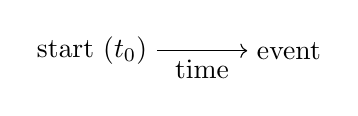
\begin{tikzpicture}
        \noindent
        \node (a) at (2.5, 0) {event};
        \node (b) at (0, 0) {start (\(t_0\))}; 
        \draw[->] (b) -- (a) node[midway, below] {time};
    \end{tikzpicture}
    \end{center}
}% ←

In the prior chapter, 
I provided and  overview of machine learning and neural networks,
highlighting central ideas and concepts releveant to the research presented
in this thesis.
Specifically, neural networks were employed in
were used in \studyii{} and \studyiii{} to develop
prediction models for ischemic heart disease.
These models, however, diverge from classical neural network methods
in that they include adaptions that that render them suitable for
modelling and prediction of time-to-event data.
This chapter delves into the fundamentals of survival analysis,
subsequently detailing the theoretical approaches used for implementing
survival analysis in neural network models.

\section{Introduction to Survival Analysis}

Generally, 
survival analysis is the collection of statistical methods
for the modelling and analysis of time-to-event data,
which is a type of data where the outcome variable of interest 
is the time until \enquote{something} happens.~%
~\autocite{kleinbaumSurvival2011}
This \enquote{something} is a particular event of interest,
which, depending on the type of analytical problem, 
could be cancer relapse, 
diabetes remission,
or death.

In cardiovascular research, 
common examples of time-to-event outcomes include
\begin{enumerate*}
    \item time to death attributed to any cause (all-cause mortality)
    \item time to death due to a specific cause (e.g. sudden cardiac arrest)
    \item time to first occurence of a \ac{MACE}
\end{enumerate*}.

To figure out what processes and characteristics 
that are associated with these events, 
in survival analysis, we try to model the relationship between
explanatory variables and the number of weeks, months, or years 
until that particular event is likely to occur. 

% marginnote→
\marginnote{%
    Survival analysis have applications outside biomedical research.
    In engineering, it is called \textit{reliability analysis} and
    is used to model the time-to-failure of system-critical components 
    such as e.g. bearings or valves.
}% ←

Although this task can be daunting in its own right, 
an additional complication to survival analysis 
is the presence of observations that are subject to 
censoring.
This concept, censoring, refers to cases 
where the event of interest has not been observed 
before the end of follow-up, 
e.g. when a study or experiment has to be stopped.
In such cases, 
we would know that a given subject did not experience a relapse 
in the three months he or she was included in the study, 
but after the study period ends, 
we have no information on the status of the patient. 
Including and utilizing this partial information
is a cornerstone in many survival analysis problems.

There exists different forms of censoring,
such as right censoring, left censoring, and interval censoring.
In the study designs used throughout this thesis 
we have only had to deal with right censoring,
the most common form of censoring,
so the two other types will not be described further.
See instead the text book by \citeauthor{kleinSurvival2003} 
for more details on this.
~\autocite{kleinSurvival2003}

\section{Fundamentals of Survival Analysis}

In survival analysis, 
the central outcome variable is survival time,
a non-negative random variable denoted as \(T\). 
When refering to specific values of \(T\), 
a lower case \(t\) is typically used.  
A survival dataset \(\mathfrak{D}\) of size \(N\) is given by
\begin{equation}
    \mathfrak{D}_N = \{(t_i, \sigma_i, \vec{x}_i) \mid i = 1, \ldots, N\} 
\end{equation}
where \(t_i = \min(T_{i}, C_i) \) is the survival time 
for the \(i\)th subject,
with \(T_i\) denoting the survival time
and \(C_i\) denoting the censoring time. 
Also, \(\vec{x}_i = (x_1, x_2, \dots, x_p)'\) is the covariate vector
and \(\sigma_i\) is the event indicator, which is defined as
\begin{equation}
    \label{eq:sigma-def}
    \sigma_i =
        \begin{cases}
            0 & \text{if subject is censored} \; (T_i >    C_i) \\
            1 & \text{if event is observed} \; (T_i \leq C_i)
        \end{cases}
\end{equation}

In the following, I will initially be assuming that \(T\) is 
continuous and that there is an absence of competing risks, 
however both of these assumptions will later be relaxed in the discussion 
of competing risks and discrete-time survival analysis.

\subsection{Basic Survival Quantities}
\label{sub:survival-quantities}

% figure: theoretical survival function{{{
\begin{marginfigure}%
	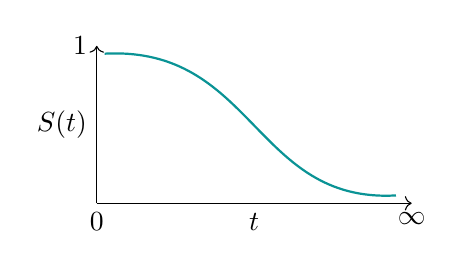
\begin{tikzpicture}[scale=2]
	  \draw[->] (0, 0) --  (2,0) 
		node[pos=0.0, below] {$0$}
		node[pos=0.5, below] {$t$}
		node[pos=1.0, below] {$\infty$};
	  \draw[->] (0, 0) --  (0,1) 
		node[pos=1.0, left] {$1$}
		node[pos=0.5, left] {$S(t)$};
	  \draw[-, color=color2, thick] 
		(0.05, 0.95) .. controls (1, 1) and (1, 0) .. (1.90, 0.05);
	\end{tikzpicture}
    \caption[A theoretical survival function]}}

In survival analysis, 
the central function of interest is 
the survival function \(S(t)\), 
that represents the probability 
of an individual still being alive after 
some specified duration of time, we have that 
%
\begin{equation}
    S(t) = \PR (T > t), \quad 0 < t < \infty.
\end{equation}

The survival function is 
the integral of the probability density function, \(f(t)\),
and is the complement to the cumulative distribution function, \(F(t)\),
which means that
~\autocite{kleinSurvival2003}
%
\begin{equation}
    S(t) = 1 - F(t) 
    \quad \text{and} \quad 
    S(t) = \int_{t}^{\infty} f(u) \, \diff u
\end{equation}

Another fundamental quantity is the hazard function, or hazard rate,
which represents the instantaneous failure rate at a given timepoint,
and is defined as
%
\begin{equation}
    \label{eq:hazard-function}
    \lambda(t) = \lim_{\Delta t \to 0} 
        \frac{\PR (t \leq T < t + \Delta t \mid T \geq t)}{\Delta t}
\end{equation}
% 
from which it can be shown that
~\autocite{kleinSurvival2003}
%
\begin{equation}
    \lambda(t) = \frac{f(t)}{S(t)} = -\frac{\diff}{\diff t} \ln[S(t)].
\end{equation}
%
and thus the hazard function completely describes the distribution of \(T\),
such that all the the other quantities can be obtained from it---%
as well as the other way around.

In terms of its interpretation, 
from \cref{eq:hazard-function} it follows that \(\lambda(t)\Delta t\) 
is a measure of the conditional probability of failure in a small time
window, given that the individual is still alive at time \(t\).
~\autocite{kleinSurvival2003}

Analogous to the relation between \(f(t)\) and \(F(t)\), 
integrating \(\lambda(t)\) with respect to \(t\),
we obtain cumulative hazard function, defined as
%
\begin{equation}
    \Lambda(t) = \int_{0}^{t} \lambda(u) \, \diff u = -\ln[S(t)].
\end{equation}

\subsection{The Kaplan-Meier Estimator}

The survival function of a population
can be estimated using the Kaplan-Meier method,
which is the standard estimator of the survival function.
~\autocite{kaplan1958nonparametric}
~\autocite{kleinSurvival2003}
In order to estimate the survival function, 
in the Kaplan-Meier method we first order
the distinct failure times such that%
\sidenote{%
    Following the example of [\cite{kleinbaumSurvival2011}], 
    the \(t\)'s denoted with subscripts within parentheses \(t_{(j)}\)
    refers to the \(j\)th element of the ordered distinct failure times and
    are thus different from \(t_1, t_2, \ldots, t_i\) that refers to the 
    observed failure time of subject \(1\), \(2\), and \(i\)
}
\begin{equation*}
    t_{(1)} < t_{(2)} < \ldots < t_{(j)},
\end{equation*}
%
and we introduce two quantities to keep track of
the number of failures/events at each timepoint \(\widebar{D}(j)\), 
as well as the number of subjects still at risk at each timepoint \(\widebar{A}(j)\).
They are defined as
\begin{equation}
\begin{aligned}
    \bar{D}(j) &= \card \{i \in \{1, \dots, n\} \mid t_i = t_{(j)}, \sigma_i = 1\} \\
    \bar{A}(j) &= \card \{i \in \{1, \dots, n\} \mid t_i > t_{(j)}\}.
\end{aligned}
\end{equation}

With these two quantities in place, 
the Kaplan-Meier estimator can then be formulated as 
%
\begin{equation}
    \widehat{S}(t)
    =   \prod_{j \mid t_{(j)} \leq t} 
        \frac{
            \bar{A}(j) -
            \bar{D}(j)
        }{
            \bar{A}(j)
        }
    =   \prod_{j \mid t_{(j)} \leq t} 
        1 - \frac{
            \bar{D}(j)
        }{
            \bar{A}(j)
        }.
\end{equation}

While the Kaplan-Meier estimator is very useful 
for estimating the average survival of a population, 
it does not account for the effect of covariates.
Instead, another approach is needed for regression analyses.

\subsection{Cox's Proportional Hazards Model}

To describe and model the relationship between explanatory variables
and time-to-event phenomenons, a widely used statistical model is 
the Cox proportional hazards model. 
~\autocite{coxRegression1972}
This model seeks to model the hazard function over time \(t\),
of an individual with a covariate vector \(\vec{x} = (x_1, x_2, \dots)'\),
and assumes that it takes the form of
%
\begin{equation}
    \label{eq:cox}
    \widehat{\lambda} (t \,|\, \vec{x}) = \hzt \exp [g(\vec{x})],
\end{equation}
%
where \(\hzt\)
is an unspecified baseline hazard function,
and \(g(\vec{x})\) is some parametric function.
For this reason, the Cox model 
is referred to as a semi-parametric model.
In its classical formulation, 
this function is a linear combination of parameters 
\(\vec{\beta}\) and covariates \(\vec{x}\),
as given by

\begin{equation}
    g(\vec{x}) 
    = \vec{\beta}' \vec{x} 
    = \beta_1 x_1 + \beta_2 x_2 + \ldots + \beta_p x_p
\end{equation}

In estimation of the parameters \(\vec{\beta}\),
the baseline hazard \(\hzt\) is treated as a nuisance function
and the coefficients are estimated by
maximising a partial likelihood
in which \(\hzt\) has been abstracted away.
~\autocite{kalbfleischStatistical2002}

A central assumption in the Cox model, 
at least in the standard version with fixed covariates
(\(\vec{\beta}\) instead of \(\vec{\beta}(t)\)),
is that of proportional hazards.
Let \(\vec{x}\) and \(\vec{x}'\) be two different 
covariate vectors, now the ratio between their
respective Cox-estimated hazards is

\begin{equation}
    \label{eq:hazard-ratio}
    \begin{aligned}
    \frac%
        {\widehat{\lambda}(t \,|\, \vec{x} \hfill)}%
        {\widehat{\lambda}(t \,|\, \vec{x'})}
    &=
    \frac%
        {\hzt \exp (\vec{\beta}\cdot\vec{x}\hfill)}%
        {\hzt \exp (\vec{\beta}\cdot\vec{x'})} \\
    &=
    \frac%
        {\exp (\vec{\beta}\cdot\vec{x}\hfill)}%
        {\exp (\vec{\beta}\cdot\vec{x'})} \\
    &= \exp (\vec{\beta} \cdot (\vec{x} - \vec{x'}))
    \end{aligned}
\end{equation}

Since the right-hand side of the equation does not include a term for \(t\),
the hazard ratio between the two samples are constant and 
they are thus proportional to one another.
This shows that by assuming the hazard takes the form of \cref{eq:cox},
then it is also assumed that the hazards between two subjects are proportional.
Although this assumption is a strong one, 
and the validity of the Cox model relies on it, 
the assumption makes interpretation of parameters easier.
~\autocite{tutzModeling2016}
For example, 
in an randomized clinical trial
studying the survival effect of a new type of medication, 
we can let \(x = 1\) represent the experimental treatment  
and \(x' = 0\) represent standard of care, 
then the hazard ratio in \cref{eq:hazard-ratio} takes the form of
%
\begin{equation}
      \exp \left(\beta (x - x')\right)
    = \exp \left(\beta (1 - 0)\right)
    = \exp (\beta ),
\end{equation}
%
which means that if \(\beta < 0\), 
then the hazard of the experimental treatment is 
\(\exp({\beta})\) times lower than standard of care
and should therefore be preferred.%
\sidenote{% 
This example is a slightly modified version of the 
one given in \cite[pp. 50]{tutzModeling2016}}


\section{Time-to-Event Prediction}

Up until now, 
I have outlined various concepts foundational to survival analysis,
focusing primarily on quantities and statistics of time-to-event outcomes
at a population level.
These measures play an important role in understanding 
and interpretation of survival data.

In the context of precision medicine, however,
the emphasis shifts towards making individualized predictions
taking distinct patient-level characteristics into account.
Consequently, as described in \cref{chap:machine-learning}, 
the primary concern lies in 
making accurate predictions on unseen data,
rather than in the exploration of disease etiology and underlying mechanisms.

For prediction of time-to-event outcomes, classical approaches 
include models based on the previously presented semi-parametric Cox model 
as well as various parametric survival models, 
such as those based on exponential, Weibull, or log-normal distributions.
~\autocite{kleinSurvival2003}
This thesis, however, 
explores the use of contemporary machine learning methods 
in time-to-event prediction,
with a particular emphasis on the application of neural networks.

\subsection{Neural Networks and Time-to-Event Outcomes}

The first application of neural networks for time-to-event prediction
was demonstrated by
\citeauthor{faraggiNeural1995} in
\citeyear{faraggiNeural1995},
and involves parameterising the parametric part of the Cox model
with a neural network, 
such that the \(g(\vec{x})\) term in \cref{eq:cox} is a 
flexible neural network model instead of a simple linear function.
\autocite{faraggiNeural1995}

\vspace{.5em}
\begin{equation*}
    \widehat{\lambda} (t \,|\, \vec{x}) = \hzt \exp [
    \eqnmarkbox[color2]{node1}{
        g(\vec{x})
    }]
\end{equation*}
\annotate[yshift=.6em]{left}{node1}{use neural network}

This approach was later further refined
in the \emph{DeepSurv} paper from 
\citeyear{katzmanDeepSurv2018a},
in which modern neural network techniques
were added to Faraggi-Simon framework, 
which markedly improved its usefulness.
~\autocite{katzmanDeepSurv2018a}
\citeauthor{katzmanDeepSurv2018a} showed that the flexibility 
offered by neural networks led to increased performance
in both synthetic and real-life time-to-event prediction applications
compared to a standard Cox model.
However, the \emph{DeepSurv} approach is still limited by the 
assumption of proportional hazards.

\subsection{Overview of Approaches}

Recently, there have been considerable interest in neural network-based
time-to-event prediction models, and as a consequence, many new methods 
have since been developed.
For a thorough overview of the existing approaches, 
\textcite{wiegrebeDeep2023} and 
\textcite{kvammeContinuous2021} provide valuable insights.
Generally, two prevailing types of approaches exists:
continuous-time methods based on the Cox model, 
which includes \emph{DeepSurv},
and discrete-time methods as exemplified by 
\textcite{leeDeepHit2018} and \textcite{gensheimerScalable2019}.

The discrete-time approaches offer several advantages that 
make them particularly relevant for neural network. 
Furthermore, they have been shown to offer better predictive
performance compared to the Cox-based methods.
~\autocite{kvammeContinuous2021, leeDeepHit2018, gensheimerScalable2019}
Notably, \emph{DeepHit}\autocite{leeDeepHit2018}
and \emph{Logistic-Hazard}\autocite{gensheimerScalable2019}
are the two most cited papers in this context as of the time of writing.
Among these and other tested approaches,
\textcite{kvammeContinuous2021} found that 
DeepHit offers excellent discrimination but suffers from poor calibration.
In contrast, the Logistic-Hazard model have nearly as good discrimination
and also significantly better calibration. 
Consequently, the Logistic-Hazard model, and an extension hereof, 
was chosen for application in 
\studyii{} and \studyiii{}.

In the following section, I will be giving a brief description of
this discrete-time formulation of time-to-event analysis and 
elaborate on the Logistic-Hazard model in more detail.

\section{Discrete-Time Survival Analysis}
\label{sec:disctime-survival}

Most textbooks on survival analysis treats survival time as continuous, 
and that is also usually the case across the biomedical litterature.
However, handling time as a something discrete can be advantegous.
In practice, most measurements of time is inherently discrete 
with durations being recorded in, for example, days; months; and weeks.
The continuous time approaches presented earlier in this chapter, 
are also applicable to discrete time data,
however, methods designed specifically for discrete time-to-event 
data have some advantages~\autocite{tutzModeling2016}:

\begin{itemize}
    \item If observed event times are inherently discrete, 
        then modelling them as such is arguably more appropriate. 
    \item In the discrete-time setting, hazards can be formulated as 
        conditional probabilities which are much more intuitive to 
        both interpret and understand.
    \item Discrete time-to-event models are more easily transferred to 
        other more general purpose modelling frameworks 
        such as generalized linear models, random survival forests, 
        neural networks.
\end{itemize}

The latter point is the main motivation behind both 
the \emph{DeepHit} and \emph{Logistic-Hazard} approach.
For a complete overview of the theory enabling these two approaches,
the book by \textcite{tutzModeling2016} is a valuable resource, 
and serves as the main source of reference for the following.

\subsection{Notation and Definitions}

In the discrete-time framework, 
continuous follow-up time \(\Tic\) is divided into \(q\) contiguous intervals,
that is
%
\begin{equation*}
	(0, a_1], (a_1, a_2], \dots, (a_{q-1}, a_q]
\end{equation*}
%
and \(\Tid \in \{1, \dots, q\}\) is a discrete random  variable
such that if \(\Tid = \tid\) is observed, then the event 
falls in the interval \((a_{\tid-1}, a_{\tid}]\).
Similarly, the discretized censoring time is \(\Cid \in \{1, \dots, q\}\).

With this discrete time scale, 
the distribution of \(\Tid\), 
given some vector of covariates \(\vec{x}\),
can be described using discrete equivalents of the previously 
outlined basic quantities of survival analysis, that is
%
\begin{align}
    \text{probability mass function:} \qquad
    f(\tid \giv \vec{x}) 
    &= \PR (\Tid = \tid \mid \vec{x}) \\
    %
    \text{cumulative mass function:} \qquad
    F(\tid \giv \vec{x}) 
    &= \PR (\Tid \leq \tid \mid \vec{x}) \\
    %
    \label{eq:discrete-hazard}
    \text{hazard function:} \qquad
    \lambda(\tid \giv \vec{x}) 
    &= \PR (\Tid = \tid \mid \Tid \geq \tid, \vec{x}) \\
    %
    \text{survival function:} \qquad
    S(\tid \giv \vec{x}) 
    &= \PR (\Tid > \tid \mid \vec{x})
\end{align}

\subsection{The Logistic-Hazard Model}

\Citeauthor{gensheimerScalable2019}'s approach, 
which they refer to as \enquote{Nnet-survival},
~\autocite{gensheimerScalable2019}
is more accurately characterized as the Logistic-Hazard method, 
as described in \textcite{kvammeContinuous2021}.
In the Logistic-Hazard method, 
the time-to-event data is described by 
modelling the effect of covariates on the discrete hazard function 
(\cref{eq:discrete-hazard}) 
using a neural network.
The concept is not novel, 
employing the discrete hazard for statistical modeling is a common method, 
as covered extensively in \textcite{tutzModeling2016}. 
In addition, a neural-network based model with the same general idea 
was presented by \citeauthor{brownUse1997} in 1997.
~\autocite{brownUse1997}
However, 
\citeauthor{gensheimerScalable2019} were the first to adapt the approach
to current neural network methodologies.

\subsection{Log-Likelihood of the Discrete Hazard}

Let \(\mathfrak{D}_{\mathrm{d}}\) 
be a discrete-time survival dataset of size \(N\),
\begin{equation}
    \mathfrak{D}_{\mathrm{d}} = 
    \{(\tid_i, \sigma_i, \vec{x}_i) \mid i = 1, \ldots, N\},
\end{equation}
where \(\tid_i\) is the discretized survival time, 
\(\sigma_i\) is the event indicator as defined in \cref{eq:sigma-def},
and \(\vec{x}_i = (x_1, x_2, \dots, x_p)'\) is the feature vector.
With the assumption of \emph{noninformative censoring},
~\autocite{kalbfleischStatistical2002}
in the Logistic-Hazard model, 
the contribution of the \(i\)th individual to the likelihood function
can be shown to be  
~\autocite{tutzModeling2016}
\begin{equation}
    \Lik_i = %
    \begin{cases}
        \PR (\Tid_i = \tid_i) & \text{if non-censored} \\
        \PR (\Tid_i > \tid_i) & \text{if censored}.
    \end{cases}
\end{equation}

These two probabilities can be expressed using the discrete hazards,
as it can be seen that
\begin{align}
    \begin{split}
    \PR (\Tid = \tid) 
    &= \PR (\Tid = \tid \mid \Tid \geq \tid) \PR (\Tid  \geq \tid) \\
    &= \PR (\Tid = \tid \mid \Tid \geq \tid) \PR (\Tid  > \tid - 1) \\
    &= \lambda (\tid) \, \prod_{s=1}^{\tid - 1} (1 - \lambda(s))
    \end{split} \\
    \intertext{and similarly}
    \begin{split}
    \PR (\Tid > \tid) 
        &= \PR (\Tid > \tid \mid \Tid \geq \tid) \PR (\Tid  \geq \tid) \\
        &= (1 - \PR (\Tid = \tid \mid \Tid \geq \tid)) \PR (\Tid  \geq \tid) \\
        &= (1 - \PR (\Tid = \tid \mid \Tid \geq \tid)) \PR (\Tid  > \tid - 1) \\
        &= \prod_{s=1}^{\tid} (1 - \lambda(i)).
    \end{split}
\end{align}

Now, by introducing an indicator function, 
defined according to \textcite{tutzModeling2016} as 
\begin{equation}
    \label{eq:lh-indicator}
    \bar{y}_i(\tid) = \begin{cases}
        1, & \text{if individual fails in \((a_{\tid-1}, a_{\tid}]\),} \\
        0, & \text{if individual survives \((a_{\tid-1}, a_{\tid}]\),}
    \end{cases}
\end{equation}
and by including the discrete hazard function and the covariates, 
the likelihood contribution for the \(i\)th individual can be expressed as
\begin{equation}
    \label{eq:lh-likelihood}
    \Lik_i = \prod_{s=1}^{\tid_i} 
        \lambda(s \giv \vec{x}_i)^{\bar{y}_i(s)}
        (1 - \lambda(s \giv \vec{x}_i))^{1 - \bar{y}_i(s)}.
\end{equation}

The total log-likelihood of all datapoints then gives the loss-function
used in the Logistic-Hazard model, 
~\autocite{gensheimerScalable2019, tutzModeling2016}
which can be expressed
\begin{equation}
    \label{eq:lh-loglikelihood}
    \lik = 
        \sum_{i = 1}^{N} 
            \sum_{s=1}^{\tid_i} 
                \bar{y}_i(s) \log (\lambda(s\giv\vec{x}_i))
                + (1 - \bar{y}_i(s)) \log (1 - \lambda(s\giv\vec{x}_i)).
\end{equation}

\subsection{Loss Function Explained}

\def\y#1#2{\hat{\lambda}_{#1#2}}
\def\yy#1#2{1\!-\!\y{#1}{#2}}

As an example, the following set of observations with discretized 
time-to-event data with a single risk, e.g. all-cause mortality, 
and a follow-up time that have been discretized into seven contiguous intervals,
constitutes a survival dataset.

\begin{equation}
\begin{tabular}{r  ccccc}
    \toprule
    subject   \(i\)      & 1 & 2 & 3 & 4 & 5 \\
    \midrule
    time    \(\tau_i\)   & 5 & 7 & 4 & 5 & 3 \\
    event   \(\sigma_i\) & 1 & 1 & 0 & 0 & 1 \\
    \bottomrule
\end{tabular}
\end{equation}

In this setting,  using the Logistic-Hazard model, 
the neural network output for this dataset is a 2-dimensional
matrix with \(5\) rows  (subjects) and \(7\) columns (time intervals),
and each entry is the predicted conditional hazard for the
specific subject at a specific timepoint. We can write this as
\begin{equation}
\hat{\bm{\Lambda}}= \!\!\!\!
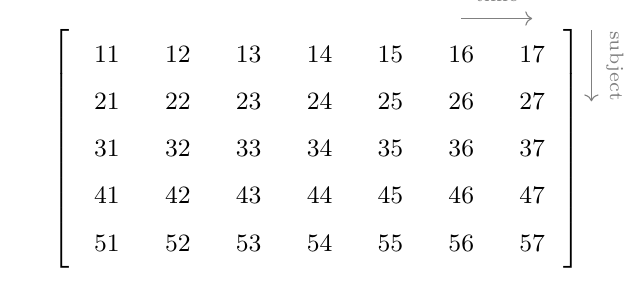
\begin{tikzpicture}
[   on grid,
    font = \small,
    baseline = -.7ex,
    inner sep=1pt,
    outer sep=0pt,
    minimum width=9mm,
    minimum height=6mm,
    every left delimiter/.style={xshift=2.5ex},
    every right delimiter/.style={xshift=-3.0ex}
]
\matrix (pred) [
	matrix of math nodes, 
    left delimiter={[}, 
    right delimiter={]},
]{ 
\y{1}{1} & \y{1}{2} & \y{1}{3} & \y{1}{4} & \y{1}{5} & \y{1}{6} & \y{1}{7} \\
\y{2}{1} & \y{2}{2} & \y{2}{3} & \y{2}{4} & \y{2}{5} & \y{2}{6} & \y{2}{7} \\
\y{3}{1} & \y{3}{2} & \y{3}{3} & \y{3}{4} & \y{3}{5} & \y{3}{6} & \y{3}{7} \\
\y{4}{1} & \y{4}{2} & \y{4}{3} & \y{4}{4} & \y{4}{5} & \y{4}{6} & \y{4}{7} \\
\y{5}{1} & \y{5}{2} & \y{5}{3} & \y{5}{4} & \y{5}{5} & \y{5}{6} & \y{5}{7} \\
};
\useasboundingbox[anchor=center] (pred.north west) rectangle (pred.south east);
\draw[->, black!50] ([xshift=2ex] pred-1-7.north east) -- ([xshift=2ex] pred-2-7.east)
    node [midway, font=\scriptsize, above, sloped] {subject};
\draw[->, black!50] ([yshift=1ex] pred-1-6.north) -- ([yshift=1ex] pred-1-7.north)
    node [midway, font=\scriptsize, above] {time};
\end{tikzpicture}
\end{equation}

Now, the indicator function can be computed 
using the defintion in \cref{eq:lh-indicator}
and the observed data \(\tid_i\) and \(\sigma_i\). 
In matrix form, the output of this function is
\begin{equation}
\bar{\bm{Y}}= \!\!\!\!
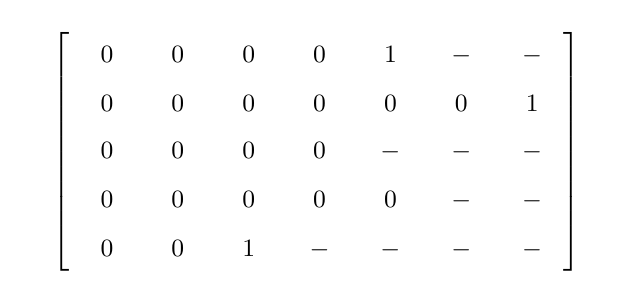
\begin{tikzpicture}
[   on grid,
    font = \small,
    baseline = -.7ex,
    inner sep=1pt,
    outer sep=0pt,
    minimum width=9mm,
    minimum height=6mm,
    every left delimiter/.style={xshift=2.5ex},
    every right delimiter/.style={xshift=-3.0ex}
]

\matrix (mask) [
	matrix of math nodes, 
    left delimiter={[}, 
    right delimiter={]}
]{ 
0 & 0 & 0 & 0 & 1 & - & - \\
0 & 0 & 0 & 0 & 0 & 0 & 1 \\
0 & 0 & 0 & 0 & - & - & - \\
0 & 0 & 0 & 0 & 0 & - & - \\
0 & 0 & 1 & - & - & - & - \\
};
\useasboundingbox[anchor=center] (mask.north west) rectangle (mask.south east);
\end{tikzpicture}
\end{equation}

Now, combining these two matrices according to the formula
in \cref{eq:lh-likelihood}, we obtain the likelihood in matrix form as
\begin{equation}
    \mathcal{L}(\bm{\hat{\Lambda}}, \bm{\bar{Y}}) = \!\!\!\!
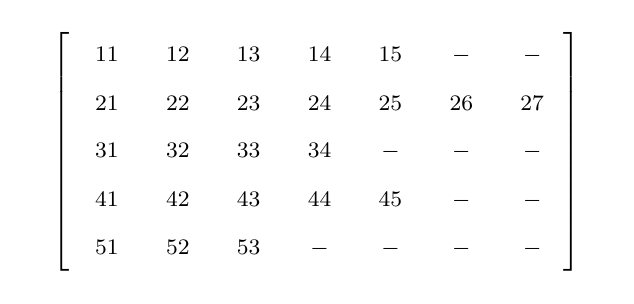
\begin{tikzpicture}
[   on grid,
    font = \small,
    baseline = -.7ex,
    inner sep=1pt,
    outer sep=0pt,
    minimum width=9mm,
    minimum height=6mm,
    every left delimiter/.style={xshift=2.5ex},
    every right delimiter/.style={xshift=-3.0ex}
]
\matrix (loss) [
	matrix of math nodes, 
    left delimiter={[}, 
    right delimiter={]},
    nodes={font=\footnotesize}
]{ 
\yy{1}{1} & \yy{1}{2} & \yy{1}{3} & \yy{1}{4} & \y{1}{5}  & -         & -         \\
\yy{2}{1} & \yy{2}{2} & \yy{2}{3} & \yy{2}{4} & \yy{2}{5} & \yy{2}{6} &  \y{2}{7} \\
\yy{3}{1} & \yy{3}{2} & \yy{3}{3} & \yy{3}{4} & -         & -         & -         \\
\yy{4}{1} & \yy{4}{2} & \yy{4}{3} & \yy{4}{4} & \yy{4}{5} & -         & -         \\
\yy{5}{1} & \yy{5}{2} & \y{5}{3}  & -         & -         & -         & -         \\
};
\useasboundingbox[anchor=center] (loss.north west) rectangle (loss.south east);
\end{tikzpicture}
\end{equation}
from which the log-likelihood, \cref{eq:lh-loglikelihood}, is then
\begin{equation*}
    \small
\begin{split}
    \mathscr{l}(\bm{\hat{\Lambda}}, \bm{\bar{Y}})
    &={} \log (\yy{1}{1}) + \log(\yy{1}{2}) + \log(\yy{1}{3}) + \log(\yy{1}{4}) 
     +  \log(\y{1}{5}) \\ 
    &+{} \log (\yy{2}{1}) + \log(\yy{2}{2}) + \log(\yy{2}{3}) + \log(\yy{2}{4}) 
     +  \log(\yy{2}{5}) + \log(\yy{2}{6}) +  \log(\y{2}{7}) \\
    &+{} \log (\yy{3}{1}) + \log(\yy{3}{2}) + \log(\yy{3}{3}) + \log(\yy{3}{4}) \\
    &+{} \log (\yy{4}{1}) + \log(\yy{4}{2}) + \log(\yy{4}{3}) + \log(\yy{4}{4}) 
    + \log(\yy{4}{5})  \\
    &+{} \log (\yy{5}{1}) + \log(\yy{5}{2}) + \log(\y{5}{3} )
\end{split}
\end{equation*}

\section{Survival Analysis with Competing Risks}

Up to this point, the description of concepts in survival analysis has
assumed the presence of only a single event type, such as all-cause mortality
(\cref{fig:ssm}).
In practice, particularly in clinical settings, 
this single-event model can be too restrictive,
and instead one needs to consider competing risks
(\cref{fig:msm}).
By definition, a competing risk is a secondary event whose occurence 
prevents the primary event from occuring.
For example,
in a study where the primary outcome is cardiovascular mortality,
deaths from non-cardiovascular causes are a competing risk.

\begin{marginfigure}[-10em]% →
    \tikzstyle{outcome}=[%
        rectangle, rounded corners, minimum height=5mm, fill=color3
    ]
    \centering
    \begin{tikzpicture}[x=0.60\linewidth, y=1cm]
    \graph [edge quotes={font=\scriptsize, fill=white}, 
            nodes      ={draw, outcome, sloped, minimum width=1cm}]{
        alive [fill=color4] -> dead [> "\(\lambda(t)\)" ];
    };
    \end{tikzpicture}
    \caption[Single-state survival model]{
        A simple survival analysis setup 
        involves modelling a single transition between states 
        \enquote{alive} and \enquote{dead}.
    }
    \label{fig:ssm}
\end{marginfigure}% ←

\begin{marginfigure}[0em]% →
    \tikzstyle{outcome}=[%
        rectangle, rounded corners, minimum height=5mm, fill=color3
    ]
    \centering
    \begin{tikzpicture}[x=0.60\linewidth, y=0.85cm]
    \graph [edge quotes={font=\scriptsize, fill=white}, 
            nodes      ={draw, outcome, sloped, minimum width=1cm}]{
        alive [fill=color4] -> {
            cause 1 [> "\(\lambda_1(t)\)" ],
            cause 2 [> "\(\lambda_2(t)\)" ],
            cause k [> "\(\lambda_\kappa(t)\)" ],
        };
    };
    \end{tikzpicture}
    \caption[Multi-state survival model]{
        A survival analysis setup with competing risks
        involves modelling transitions between states 
        \enquote{alive} and \(k\) different absorbing
        states, \enquote{cause 1} to \enquote{cause \(\kappa\)}
    }
    \label{fig:msm}
\end{marginfigure}% ←

\subsection{Cause-Specific Survival Quantities}

To describe time-to-event phenomena with competing risks, 
we introduce the cause-specific hazard function and 
cumulative-incidence function.
With \(R \in \{1, \dots, \kappa\}\) denoting the \(\kappa\) different competing risks, 
the continuous cause-specific hazard function is defined as
\begin{equation}
    \lambda_r(t) = \lim_{\Delta t \to 0} 
        \frac{\PR (t \leq T < t + \Delta t, R=r \mid T \geq t)}{\Delta t}
\end{equation}
where \(r\) refers to a specific value of \(R\).
The cause-specific cumulative incidence function is defined as
~\autocite{kalbfleischStatistical2002}
\begin{equation}
    F_r(t) = \PR(T \leq t, R = r).
\end{equation}

The overall hazard and cumulative incidence, 
which combines failures of any of the \(\kappa\) causes,
correspond to the hazard function 
and the cumulative distribution function 
in the single-event setting, that is
\begin{equation}
    \lambda(t) = \sum_{r=1}^{\kappa} \lambda_r(t)
    \quad \text{and} \quad
    F(t) = \sum_{r=1}^{\kappa} F_r(t).
\end{equation}

\subsection{Modelling the Cause-Specific Hazard}

In the competing risks setting, 
the typical approach is to treat competing risks as censored events
and use Cox regression to estimate the cause-specific hazards.
In this approach, the cause-specific hazard takes the form of
\begin{equation}
    \hat{\lambda}_{r}(t \giv \vec{x}) 
        = \lambda_{0r} \exp(\bm{\beta}_r \cdot \bm{x})
\end{equation}
from which one can obtain the cause-specific regression coefficients 
\(\bm{\beta}_r\).
In \studyi{}, we use this to estimate the cause-specific hazards
of \ac{IHD} progression and non-\ac{IHD} mortality associated with 
different clusters of \ac{IHD} patients, 
as defined by their respective comorbidity profiles.

However, an important assumption required by all survival methods
outlined so far, including the Cox proportional hazards model,
is that of noninformative censoring.
~\autocite{kleinbaumSurvival2011}
This assumption states that the
\textquote[kleinbaumSurvival2011]{%
    probability of being censored at time \(t\) does not depend on
    prognosis for failure at time \(t\)%
}, which in the context of competing risks can be especially problematic,
since it also implies that competing failure types should be independent.
It is difficult to ascertain if this is the case from observed data, 
however if we include risk-factors that are shared by competing events,
it is possible to alleviate the bias related to this possibly erroneous
assumption.
~\autocite{kleinbaumSurvival2011}

\subsection{The Aalen-Johansen Estimator}

In estimation of the population-level cause-specific incidence,
the approach of simply treating competing events as censored 
and applying the standard Kaplan-Meier estimator, 
is generally a bad idea, since it often leads to a very biased estimate of 
\(F(t)\).
~\autocite{pepeKaplan1993}
Instead, an alternative approach is the Aalen-Johansen estimator
that allows estimation of the cause-specific cumulative incidence.
~\autocite{aalenEmpirical1978}
Of note, the Aalen-Johansen is a general method for estimating
transition probabilities in state-transition models,
and can be used to describe complex multi-state models,
including those with repeated events and with non-terminal states.
~\autocite{survival-package}
However, we will be assuming a standard competing-risk setting
with \(\kappa\) different terminal states, 
as depicted in \cref{fig:msm}.
 
If we again order the distinct failure times, 
corresponding to any cause, 
such that
\(t_{(1)} < t_{(2)} < \ldots < t_{(j)}\),
and update the definition of \(\bar{D}(j)\) to keep track of cause-specific
events, such that we have
\begin{equation}
\begin{aligned}
    \bar{D}(j, r) &= \card \{i \in \{1, \dots, n\} \mid t_i = t_{(j)}, r_i = r\} \\
    \bar{A}(j)    &= \card \{i \in \{1, \dots, n\} \mid t_i > t_{(j)}\}.
\end{aligned}
\end{equation}
Now, the Aalen-Johansen estimator of the cumulative incidence function
can be defined as 

\begin{equation}
    \widehat{F}_r(t)
    =   \sum_{j \mid t_{(j)} \leq t}{
        \!\!
        \widehat{S}(t_{(j-1)})
        \frac{\bar{D}(j, r)}{\bar{A}(j)}
    }
\end{equation}
  
\chapter{Overview of Data Resources}

Data stands as the cornerstone of both precision medicine and machine learning.
Its availability is crucial; without it, research in these
fields would be almost impossible. 
The emergence of high-throughput analyses and \acp{EHR} has 
led to a Cambrian explosion of the volume of data being generated,
which has the potential of revolutionizing the 
entire landscape of biomedical research. 
However, the sensitive nature of this data means
that access is frequently a major challenge, 
often serving as a major bottleneck in
many research endeavors.

In the context of the studies conducted for this thesis, I have been in the
privileged position of working within a research group where permissions, 
data access, and the necessary infrastructure were already well-established.
In terms of infrastructure, a key aspect of our data handling involved the use 
of a secure high-performance computing environment. 
This not only ensured the efficient processing of large datasets and 
training of large neural networks, 
but also maintained the highest standards of data security and
confidentiality, which are paramount in dealing with sensitive health records.
These aspects have been instrumental in enabling and driving 
the research and analyses presented in this thesis.

Focusing on the data itself,
this chapter aims to provide a comprehensive overview of the various data
sources utilized in the studies comprising this thesis. It details the
databases and registries that were accessed and analyzed,
highlighting how each contributed to the research. 

\section{The Danish Civil Registration System}

\Ac{CPR} is the central administrative register in Denmark,
and stores personal information on the entire Danish population,
including birth date, sex, addresses, vital status, 
and, importantly, a unique personal identification number, 
known as \enquote{\ac{CPR}-nummer} or \enquote{personnummer}.
~\autocite{schmidtDanish2014}
The \ac{CPR} number is assigned at birth or upon obtaining Danish citizenship, 
and have been in use since 1968.
As of January 2, 2014, 
\num{9484792} \ac{CPR} numbers were assigned.
~\autocite{schmidtDanish2014}
Of these \num{5685912} were \enquote{active},
and \num{3798880} were \enquote{non-active},
the latter primarily attributed to death and emigration.
~\autocite{schmidtDanish2014}

In Denmark, the \ac{CPR} number is as essential as a bicycle, 
required for opening a bank account, 
borrowing a library book, 
getting treated for appendicitis, and everything in between.
This widespread use, 
combined with the country's long-standing tradition
of organising and keeping record of detailed data in 
administrative databases and registries,
have enabled the construction of a large network
of interlinkable epidemiological resources.
~\autocite{schmidtDanish2019}
In this light, the whole nation can be utilized as a research cohort
as outlined by \textcite{frankEpidemiology2000} in a letter
to \textit{Science}.

\section{The Danish National Patient Register}

Of the Danish registries, \ac{LPR} is arguably one of the most important.
\ac{LPR}, or \enquote{Landspatientregisteret}, 
is a comprehensive clinical register that has
been instrumental for clinical research and administration in Denmark,
and serves multiple critical functions.
~\autocite{schmidtDanish2015}
Primarily, it underpins the Danish Health and Medicines Authority's hospital
statistics and is a main foundation for health economic calculations.
Additionally, the \ac{LPR} is instrumental in monitoring the
prevalence of various diseases and treatments. 
Furthermore, the registry plays a key role in
facilitating quality assurance of Danish healthcare services and provides
hospital physicians access to patients' hospitalization histories, enhancing
patient care and treatment efficacy.
~\autocite{schmidtDanish2015}
The register is updated monthly based on reports from the hospitals,
and has been collecting data continuously since 1977.
~\autocite{schmidtDanish2015}

\subsection{Content and Structure}

The \ac{LPR} encompasses a wide array of data on each individual, 
such as personal information, admission and discharge details, diagnoses, 
examinations, treatments including surgeries, information on accidents, 
and additional details concerning births. 
~\autocite{schmidtDanish2015}
The information in the register is organised in a
structured format with different data types being stored 
in distinct tables that can be linked following a 
specified relational data model.
~\autocite{lpr2dok}

This data model, referred to as \acsfont{LPR2},  
have remained largely unchanged since the release of the registry in 1977.
However, in early 2019, it underwent a significant overhaul to a 
new and refined data model, \acsfont{LPR3}.
~\autocite{nielsenLPR32018}
The \acsfont{LPR3} model addresses certain limitations of its predecessor, 
notably enabling the creation of more fine-grained patient care timelines. 
While the specifics of these improvements are beyond the scope of this thesis, 
it is important to note that the \acsfont{LPR3} model is not entirely 
backwards compatible with the \acsfont{LPR2} data model. 
Nevertheless, depending on the specific use case, 
it remains possible to create data extracts that are compatible
to one another.

\subsection{Classification of Diseases}

The highly structured data within the \ac{LPR} 
is coded using the national \acs{SKS} classification scheme (\enquote{\acl{SKS}}), 
a collection of Danish, international, and Nordic classification standards
maintained by the Danish Health Data Authority.
~\autocite{schmidtDanish2015}
These standards includes
the \acfi{NOMESCO} system for surgical procedures,
the \acfi{ATC} system for medication,
and the \acfi{ICD} system for diagnoses. 
~\autocite{schmidtDanish2015}

Focusing on diagnosis codes, 
the \ac{LPR} is currently using the \ac{ICD-10},
and have been doing so since the start of 1994
where it replaced the \acsu{ICD-8}.
~\autocite{schmidtDanish2015}
This transition can complicate longitudinal studies of disease occurence, 
but prior efforts by the Brunak group have succesfully
created a mapping between \ac{ICD-8} and \ac{ICD-10}
that can be used to mitigate such challenges.
~\autocite{pedersenUnidirectional2023}

The \ac{ICD-10} coding system follows a hierarchical structure 
with every code beginning with a letter followed by two or more digits.
Each code falls in one of 21 high-level categorisation of diagnoses 
that e.g.  includes chapters
(ii)~\emph{Neoplasms};
(iv)~\emph{Endocrine, Nutritional, and Metabolic Diseases};
and (ix)~\emph{Diseases of the Circulatory System}.
Using the latter as an example, 
\cref{fig:icd10-hierarchy} shows the hierarchical structure of the
\ac{ICD-10}.

% figure: icd10-hierarchy→
\begin{figure}
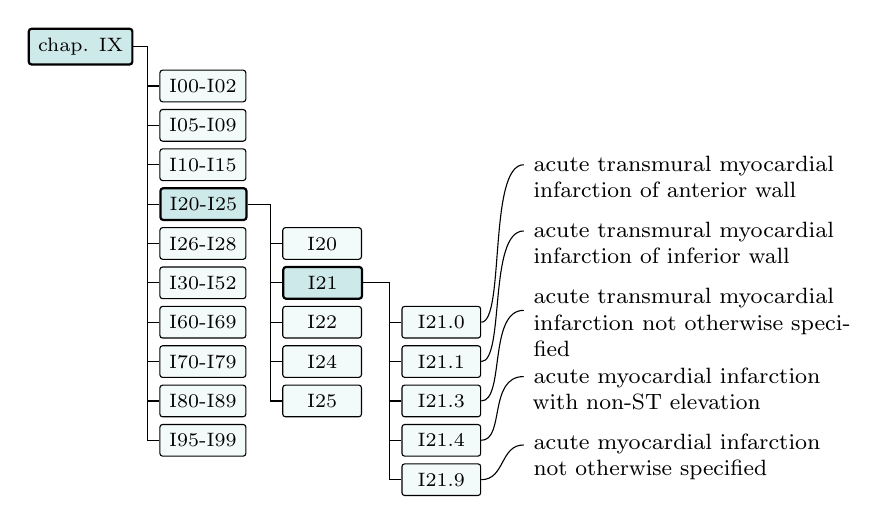
\begin{tikzpicture}[
    every node/.append style = {
        draw, anchor = west, 
        minimum width=10mm, 
        minimum height=4mm,
        font=\tlfstyle\scriptsize,
        rounded corners=1pt,
        fill=color2!5
    },
    sel/.style = {fill=color2!20, draw=black, thick},
    txt/.style = {
        fill=none, draw=none, font=\footnotesize, text width=4.0cm,
        text height=5mm
    },
    grow via three points={
        one child    at (1.0, -0.5) and 
        two children at (1.0, -0.5) 
                    and (1.0, -1.0)
    },
    edge from parent path={
        (\tikzparentnode.east) 
        -| ([xshift=-4.2]\tikzchildnode.west)
        |- (\tikzchildnode.west)
    }]
    \node[sel] {chap. IX}
        child {node {I00-I02}}
        child {node {I05-I09}}
        child {node {I10-I15}}
        child {node[sel] {I20-I25}
            child {node (i20) {I20}}
            child {node [sel] (i21) {I21}
                child {node (1) {I21.0}}
                child {node (2) {I21.1}}
                child {node (3) {I21.3}}
                child {node (4) {I21.4}}
                child {node (5) {I21.9}}
            }
            child {node {I22}}
            child {node {I24}}
            child {node {I25}}
        }
        child {node {I26-I28}}
        child {node {I30-I52}}
        child {node {I60-I69}}
        child {node {I70-I79}}
        child {node {I80-I89}}
        child {node {I95-I99}}
    ;

    \node [txt] (t1) at (6.3cm, -1.5cm) 
        {acute transmural myocardial infarction of anterior wall};
    \node [txt, below=3mm of t1.center] (t2) 
        {acute transmural myocardial infarction of inferior wall};
    \node [txt, below=3mm of t2.center] (t3) 
        {acute transmural myocardial infarction not otherwise specified};
    \node [txt, below=3mm of t3.center] (t4) 
        {acute myocardial infarction with non-ST elevation};
    \node [txt, below=3mm of t4.center] (t5) 
        {acute myocardial infarction not otherwise specified};

    \draw (1.east) .. controls +(2ex,0) and +(-3ex,0) .. (t1.west);
    \draw (2.east) .. controls +(2ex,0) and +(-3ex,0) .. (t2.west);
    \draw (3.east) .. controls +(2ex,0) and +(-3ex,0) .. (t3.west);
    \draw (4.east) .. controls +(2ex,0) and +(-3ex,0) .. (t4.west);
    \draw (5.east) .. controls +(2ex,0) and +(-2ex,0) .. (t5.west);
    
\end{tikzpicture}
\caption[The ICD-10 Hierarchy]{%
    Schematic illustrating the hierarchical structure of the \ac{ICD-10} coding
    system. 
    Using Chapter IX---which covers diseases of the circulatory system
    (codes I00-I99) and comprises ten different \enquote{blocks}---as an example, 
    the diagram shows how these blocks are segmented into 
    \enquote{level 3} codes, such as I20 to I25, 
    corresponding to ischemic heart disease. 
    It provides an expanded view of the I21 category, 
    containing specific subtypes, \enquote{level 4} codes, 
    of acute myocardial infarctions 
    from I21.0 for the anterior wall 
    to I21.9 for unspecified instances. 
    Deeper levels of the hierarchy also exists,
    but is not included in this diagram.
}
\label{fig:icd10-hierarchy}
\end{figure}
% ←

\section{The East Danish Heart Registry}

\ac{RKKP} is a program set in place to support the
management and infrastructure related to clinical quality databases.


Data from some of the other general registries, 
including the \ac{LPR}, is being used to populate 
specific variables in different \ac{RKKP} registries.

The \ac{RKKP} undergoes revision by the National Health Authority
every three years to continuously assess specific 
criteria for function, safety, and methodology.


\section{The Register of Pharmaceutical Sales}



\section{The Causes of Death Register}

When a person in Denmark dies, a doctor performs a post-mortem examination. The
doctor fills in a death certificate and reports the death by submitting the
certificate to the Danish Health Authority.

\section{The BigTempHealth Project}

\subsection{Patient Notes}

The DNPR does not contain information on tobacco usage, blood pressure, 
body-mass index, and other important covariates to consider in the
context of cardiovascular diseases.

% figure: journal text→
\begin{figure}
{
% Define new commands for each category
\newcommand{\cbox}[2]{%
    \tcbox[on line, colback=#1!50!white, boxsep=1.5pt, colframe=black,
           valign=center, left=0pt, right=0pt, top=0pt, bottom=0pt, boxrule=1pt]{#2}%
}%
\newcommand{\diag}[1]{\cbox{color3}{#1}}
\newcommand{\symp}[1]{\cbox{color4}{#1}}
\newcommand{\drug}[1]{\cbox{color5}{#1}}
\newcommand{\quan}[1]{\cbox{color6}{#1}}
\newcommand{\kwpa}[1]{\cbox{color7}{#1}}

\begin{Verbatim}[commandchars=\\\{\}, fontsize=\scriptsize, 
    frame=single, framesep=1em, numbers=left, numbersep=3pt]
68-year-old woman, no earlier known cardiovascular disease, 
referred by gp for observation of \diag{angina pectoris}.

Risk factors:
\diag{Hypertension}: Yes, newly discovered, currently well-treated.
\diag{Hypercholesterolemia}: Yes. Under treatment.
Family: No family history of \diag{ischemic heart disease}.
Smoking: Quit 15 years ago, before that 20 pack-years.
Claudication: No.

Previously:
Known since 2001 with \diag{type II diabetes mellitus}, treated 
with \drug{Metformin}.  Followed up with regular checks. 
Complications with discrete neuropathy and beginning 
macular degeneration.

Currently:
For about 3 months, \symp{intermittent pressure in the left side}
\symp{of the chest}. No radiation, independent of physical 
activity. Daily attacks lasting a few seconds. During the 
same period, has been diagnosed with \diag{severely elevated blood}
\diag{pressure}. Recently started anti-hypertensive treatment with
good effect.

Medication:
- \drug{Metformin} \quan{1000 mg} x 2
- \drug{Simvastatin} \quan{20 mg} x 1
...

Objective:
Normal general condition.
Nutritional status above average.
\kwpa{Blood pressure 149/91}, \kwpa{pulse 76}, \kwpa{height 177 cm}, \kwpa{weight 96 kg}
\end{Verbatim}
}
\caption{Artificial example of unstructured text in an \ac{EHR}}
\end{figure}% ←
    

\part{Outline of Studies}
\chapter{Study I: Comorbidity Clustering in Ischemic Heart Disease}
\label{chap:study1-outline}

In this chapter, I provide a summary of the work from \studyi{}.
I describe the background and rationale,
outline essential methodological details,
and discuss the main research findings.

The manuscript, titled \enquote{%
Subgrouping multimorbid patients with ischemic heart disease by
means of unsupervised clustering: A cohort study of 72,249
patients defined comprehensively by diagnoses prior to
presentation}, is currently under revision.
An earlier version have been deposited on the medRxiv preprint server. 
\autocite{haueSubgrouping2023}
The revised, full-length manuscript is included in 
\cref{chap:study1-paper}.

\section{Background and Rationale}

\Ac{IHD} is highly heterogeneous in its onset, burden, and progression.
As delineated in \cref{chap:precision-medicine}, its manifestations range from 
\ac{AMI} to slowly progressing chronic coronary syndromes.
This heterogeneity is partly explained, and further complicated,
by the fact that most patients with \ac{IHD} have one or more 
comorbidities.
Current clinical practice is historically mainly based on a single-disease paradigm
and thus, complexities imposed by concurrent comorbid diseases are therefore 
often overlooked.
~\autocite{formanMultimorbidity2018}

In this study, we sought to characterise the spectrum of multimorbidity
in \ac{IHD}. 
We adopted a data-driven strategy, using unsupervised machine learning
methods to identify and characterize subgroups 
with distinct comorbidity patterns. 
Our hypothesis centered on the notion that the 
variety and types of comorbidities,
here classified according to \acsu{ICD-10} codes, 
could facilitate the identification of distinct and clinically relevant 
patient clusters in \ac{IHD}.

\section{Study Design and Outcomes}

We linked the \ac{BTH} dataset to the \ac{LPR} and \ac{DAR}, 
and identified all patients with an \ac{ICD-10} code for \ac{IHD},
who underwent \ac{CAG} or \ac{CCTA} between 2004 and 2016 
(\num{72249} patients in total).
We used the date of the first \ac{CAG} or \ac{CCTA} as the index date. 
All \ac{ICD-10} codes before this date were collected
for clustering analysis, excluding any \ac{IHD} codes (\ac{ICD-10}: I20-25).

In our study, we defined two main outcomes to assess the risk
profiles of the different multimorbidity subgroups: (i) new ischemic events
and (ii) mortality from non-\ac{IHD} causes.
New ischemic events, a composite outcome, included 
(a) hospital admission for \ac{AMI} or \ac{UA} after 30 days of follow-up
(b) revascularization procedures unrelated to the index \ac{CAG}/\ac{CCTA},
and (c) any deaths with \ac{IHD} as the primary or secondary
cause registered on the death certificate.

We used days since the index procedure as the time-scale and limited 
follow-up to at most five years. The two main outcomes were treated
as competing risks.

\section{Methodology}

\begin{figure*}[tp]
    \includegraphics{graphics/clustering-overview.pdf}
    \caption[Overview of the comorbidity clustering approach]{%
        Overview of the comorbidity clustering approach in \studyi{},
        detailing the different steps going from \ac{LPR} patient record data
        to identification and characterisation of distinct 
        multimorbidity clusters. 
    }
    \label{fig:dishisclust}
\end{figure*}

The overall methodology employed in this study is illustrated 
in \cref{fig:dishisclust}. In the following, I will be outlining the 
different steps of our comorbidity clustering approach. 

In this study, we represented multimorbidity by constructing patient-level
vectors that aggregated all diagnosis codes assigned up until the index date 
(as illustrated by steps 1 and 2 in \cref{fig:dishisclust}).
We excluded \ac{IHD} codes (\ac{ICD-10}: I20-25) and
codes belonging from chapters XV, XVI, XVII, XIX, XX, and XXI.%
\sidenote{%→
    These chapters are in the Danish \ac{ICD-10} version defined as
    \begin{itemize}[itemsep=1pt, parsep=0pt]
        \item Chapter XV (O00-O99): Pregnancy, childbirth and the puerperium
        \item Chapter XVI (P00-P99): 
            Certain conditions originating in the perinatal period
        \item Chapter XVII (Q00-Q99):
            Congenital malformations, deformations and chromosomal abnormalities
        \item Chapter XIX (S00-T98): 
            Injury, poisoning and certain other consequences of external causes
        \item Chapter XX (X60-Y09): 
            External causes of morbidity and mortality
        \item Chapter XXI (Z00-Z99): 
            Factors influencing health status and contact with health services
    \end{itemize}
}
% ←
In addition, we removed rarely used codes assigned to less than five patients.

The remaining codes were then counted (step 3), 
and embedded in a vector space model 
~\autocite{saltonVector1975}
using \ac{SVD}
~\autocite{golubSingular1971} (step 4).
Next, we used these embedded patient-level vectors 
to create a patient similarity matrix (step 5). 
For this matrix, we used cosine similarity as the similarity measure,
which calculates the cosine of the angle \(\theta\) 
between the embedded vectors.

From the similarity matrix we could then 
construct a patient similarity network,
which is a weighted undirected graph with 
patients as vertices. 
The edges in the graph represents the connections between patients,
which is weighted by the similarity of their respective diagnosis vectors.
As this graph could contain a total of
\num{2609922876} edges, which is computationally intractable, 
we pruned the network by discarding low-similarity edges 
(\(\cos{\theta} \leq 0.3\)) and limited the number of edges
connected to each vertex to the \num{8000} with greatest weight.

Subsequently,
the patient similarity network,
was then subject to cluster analysis,
using the \ac{MCL} algorithm 
~\autocite{vandongenGraph2008}
(step 6). 
The clusters obtained were then characterised (step 7).
This characterisation involved four key aspects 
(i) estimation of \acp{HR} for cluster comparisons using Cox proportional hazards models,
(ii) phenotypic enrichment analysis, 
(iii) examination of clusters based on laboratory test profiles,
and (iv) testing for genetic associations through \acp{PRS}.
In the following I will limit the presentation
of results to aspects (i) and (ii), 
as these are most integral to the study,
and will otherwise refer to the full-length manuscript.

\section{Main Findings}

% \subsection{Cohort Characteristics}
% 
% The study included \num{72249} patients, 
% predominantly male (\qty{63.1}{\percent}), with a mean age of 63.9
% years. 
% The most common inclusion diagnosis was angina pectoris, followed by acute
% myocardial infarction and chronic IHD. The most common comorbidities recorded
% prior to the index \ac{CAG} or \ac{CCTA} is
% hypertension (I10.9), dyslipidemia (E78.0), 
% and non-insulin-dependent diabetes (E11.9).
% The average number of diagnoses in the patient vectors, i.e. prior to index,
% was \num{8.1}. 
% Of the entire cohort, \qty{6.7}{\percent} had no prior diagnoses registered.

\subsection{Cluster Analysis and Outcomes}

%The clustering identified 36 distinct patient subgroups 
%which in total included \qty{94}{\percent} of the cohort. 
%The patients not belonging to a cluster, 
%was primarily those without any registered diagnoses.
%We discarded clusters with a size less than 500 (4 clusters),
%since the goal was to describe the more general patterns of multimorbidity,
%and instead focused the characterisation to the remaining 31 clusters.

The clustering resulted in 31 distinct patient subgroups, 
each characterised by specific patterns of multimorbidity.
We incorporated cluster membership in Cox regression models, 
which was further adjusted for sex and age. 
This was to obtain estimates for the risk associated with the comorbidity
profiles in each cluster, beyond those patterns primarily dependent on
age or sex.
The \acp{HR} were estimated 
by contrasting each single cluster against all others.
The size of clusters, mean age at index, and average propotion of males, 
and the adjusted \acp{HR} for the two outcomes, are
depicted in \cref{fig:cluster-results}.

\begin{figure*}[t!]% →
    \includegraphics{graphics/clustering-results.pdf}
    \caption[Cluster characteristics and outcomes][0em]{%
        Cluster characteristics and adjusted hazard ratios.
        The first panel,
        from top-left to bottom-right,
        shows the number
        of patients in each cluster, 
        arranged according to their respective sizes.
        This ordering is maintained in subsequent panels.
        The second panel shows the average age at the index \ac{CAG}/\ac{CCTA},
        ranging from \qty{56.2}{years} (C25) to \qty{74.2}{years} (C10).
        The third panel shows the sex distribution in each cluster,
        using fill color to indicate the proportion of males;
        red for clusters with more than \qty{50}{\percent} females,
        and blue for those with more than \qty{50}{\percent} males.
        The fourth and fifth panels shows the adjusted hazard ratios
        for new ischemic events and non-\ac{IHD} mortality, respectively.
        Here, clusters with a red fill indicate an \ac{HR} below one,
        while those with a blue fill have an \ac{HR} above one.
        Clusters with a hazard ratio significantly different from
        one are marked with an asterisk (\(*\)).
    }
    \label{fig:cluster-results}
\end{figure*}% ←

Our analysis revealed that
certain clusters had significantly different risks compared to others.
Comorbidity profiles within five clusters (C5, C9, C18, C23, C30) were
associated with a significantly increased risk of new ischemic events.
Conversely, profiles in two clusters (C2, C3) were associated with a 
significantly reduced risk of these events. 
Twelve clusters (C4, C5, C14, C16, C17, C18, C20, C23, C24, C25,
C28, C30) had profiles associated with a significantly higher risk 
of non-\ac{IHD} mortality. 
In contrast, six clusters (C2, C3, C6, C7, C11, C13) had
profiles that were linked to a significantly lower risk of 
non-\ac{IHD} mortality.
Of note, four of the five cluster profiles with an increased risk of 
new ischemic events also exhibited an increased risk of 
non-\ac{IHD} mortality. 

\subsection{Phenotypic Characterisation of Clusters}

\begin{figure*}[tbp]% →
    \includegraphics[clip=false, trim=6mm 5mm 0 4mm]%
        {graphics/cluster-summary.pdf}
    \caption[Overview of cluster phenotypes]{%
        From manual review of the between-cluster enrichment of 
        diagnosis codes, we assigned each cluster a label based
        on its most prevalent codes.
        To aid the intrepretation, the clusters were further organized by 
        consideration of their estimated hazard ratios 
        and shared diagnostic similarity.
        Clusters marked with \uporange{} or \upblue{} have a 
        significantly increased risk of new ischemic events
        and non-\ac{IHD} mortality, respectively.
        Conversely, \downorange{} or \downblue{} marks those with
        a significantly decreased risk.
        A single arrow indicates the direction of the effect 
        and that the association was not found to be significant.

    }
    \label{fig:cluster-summary}
\end{figure*}% ←

% To describe the patterns associated with increased or 
% decreased risks, we further characterised the clusters
% and summarise our key findings here.

As a first step, we evaluated the intra-cluster prevalence of all unique diagnosis
codes (\num{3046} in total) within patient vectors. 
These prevalences was then compared with the average prevalences
across all clusters by calculating \ac{OE}-ratios, 
to pinpoint \ac{ICD-10} codes that were disproportionately represented 
in various clusters.  
The top ten most overrepresented or underrepresented codes for each
cluster are detailed in supplementary tables 5A and 5B of the manuscript
(\cref{chap:study1-paper}).

We conducted a manual review of these findings, assigning a label to each
cluster based on the associated codes. Given that multiple codes could pertain
to a single cluster, these labels are not definitive but offer a general
overview, as depicted in \cref{fig:cluster-summary}. 
Furthermore, in \cref{fig:cluster-summary}, we organise the
clusters by both their common traits and the hazard ratios 
derived from the Cox analyses.

\section{Interpretation}

From \cref{fig:cluster-summary}, 
we see that the five clusters (C5, C9, C18, C23, C30) with a 
significantly increased risk of both new ischemic events and non-\ac{IHD} mortality
were characterised by the presence of important prognostic comorbidities in \ac{IHD}:
diabetes, peripheral atherosclerosis, heart failure, 
and chronic kidney disease. 

Both diabetes and chronic kidney disease 
are highlighted as important non-cardiovascular
comorbidities in the 2019 \acsu{ESC} guidelines for chronic coronary syndromes,
and both peripheral artery disease and renal dysfunction is explicitly
described as comorbidities that negatively impact prognosis.%
\sidecite[15em]{knuuti20192020}
Heart failure, 
also known to affect prognosis and included in clinical guidelines,
is, for example, included as one of eight carefully selected predictors
in the widely used \acsfont{GRACE} risk and mortality calculator.%
\sidecite[13em]{foxShould2014}
This showcases that our framework is able to identify known comorbidites
that affect the clinical course of cardiovascular disease.
In addition, it further emphasizes the significance of these 
comorbidities and the broader concept of considering
comorbidity in clinical assessment of \ac{IHD}.

We did not identify other clusters with comorbidity profiles
that significicantly increased the risk of new ischemic events,
however, both the second and third largest clusters (C2 and C3)
were found to have comorbidities associated with a significant decreased risk
of both new ischemic events and non-\ac{IHD} mortality.
Cluster C2 is characterised by the presence of codes 
for both gallstones (K80) and abdominal pain (R10).
Cluster C3 relates to symptom codes (R00-R99),
with high \ac{OE}-ratios for
{pain in throat and chest} (R07.9), 
{other chest pain} (R07.3), 
and {muscle strain} (M62.6).

It is interesting that the second largest cluster (C2)
is characterised by gallstones as a comorbid condition.
Many studies have previously reported a link between
gallstones and ischemic heart disease,
\autocite{zhengGallstones2016}
\autocite{upalaGallstone2017}
\autocite{wirthPresence2015}
however, the underlying reasons for this association remain
somewhat unclear and it is uncertain the link is causal.
It is known that the two diseases shares pathogenicity factors,
which include hypercholesterolemia, diabetes, and hypertension,
so parts of the pathological mechanism is likely shared.
\autocite{zhengGallstones2016}

In our study, focusing on patients with incident \ac{IHD},
the presence of gallstones appear to positively affect prognosis.
A possible explanation is that acute symptoms of gallstone disease
can immitate heart disease symptoms, and thus, the cluster could be 
enriched for patients that may not have \ac{IHD} to begin with.
This area warrants further investigation to better understand these connections
and their implications for clinical practice.

Two clusters were characterised by the co-occurence of cancer comorbidities.
Clusters C24 and C28 were enriched for breast and prostate cancer, 
respectively.
Our current methodology does not distinguish between active cancer
or if the patient has been cured, which represents a key limitation
of the approach.
However, both clusters were found to have an increased risk of 
non-\ac{IHD} mortality.

In patients with active cancer,
the management of \ac{IHD}, and specifically \ac{ACS}, 
is challenged by increased risk of bleeding,
low platelet count, and increased thrombotic risk.
~\autocite{byrne20232023}
Furthermore, 
many chemotherapeutic agents have cardiotoxic side effects,
as discussed in a 2016 \ac{ESC} position paper on the 
cardivascular toxicity of cancer treatment.
~\autocite{zamorano20162016}
Moreover,
studies indicate that radiotherapy breast cancer
is associated with an increased risk of developing \ac{IHD}, 
in a dose-dependent manner.
~\autocite{darbyRisk2013}
This underscores the complex balancing act involved in concurrently managing
both conditions, where the treatment of one disease can potentially exacerbate
the other.

\section{Conclusion}

In this study, we presented a large-scale data-driven approach
for analysis of comorbidity patterns in more than \num{70000} adult 
patients with incident \ac{IHD}.
We took a hypothesis-free approach and used a broad definition of 
multimorbidity, including more than \num{3000} different \ac{ICD-10} codes in
the decription of prior and coexisting comorbidities in \ac{IHD}.
Using unsupervised clustering, we identified disctinct groups of patients 
each characterised by specific patterns of multimorbidity and associated
risks of both disease progression and mortality from unrelated causes.

Using this approach, we were able to identify clusters characterised by
the presence of well-established prognostic comorbidities, including
diabetes, peripheral atherosclerosis, heart failure, and chronic kidney
disease. 
All clusters associated with these diseases
were all found to be significantly associated with an 
increased risk of adverse events. 
These findings thus represents a form of positive control
which supports the validity of the described methodology.

It is important to emphasize that the presented clustering is not
intended to provide the definitive or universally applicable 
multimorbidity subgroups in \ac{IHD}. 
Instead, the purpose and implication is to provide a valuable tool
for the data-driven exploration of real-world multimorbidity patterns
in \ac{IHD}.
As such, it can be used for generating hypotheses and can likely inform
and guide future research on multimorbidity-informed
treatment and management of \ac{IHD}.

Mapping out the landscape of multimorbidities in a real-world cohort of 
patients with \ac{IHD}, could inform clinical managment and could serve
as a tool for identification of comorbidity combinations for which
current clinical knowledge is currently limited.
Strict inclusion and exclusion criteria in many \acp{RCT} 
potentially limit the applicability of existing \ac{IHD} 
management guidelines on patients with pronounced multimorbidity.
~\autocite{richKnowledge2016}
To adress such limitations, an important first step is to obtain an overview
of the specific patterns of multimorbidity associated with \ac{IHD}.
 
\chapter{Study II: Time-to-Event Prediction of All-Cause Mortality}
\label{chap:study2-outline}

\newcommand{\graceii}{\acsfont{GRACE 2.0}}

In this chapter, I provide a summary of the work from \studyii{}.
I describe the background and rationale,
outline essential methodological details,
and discuss the main research findings.

The manuscript, titled \enquote{%
Development and validation of a neural network-based survival model 
for mortality in ischemic heart disease}, 
is currently under review (2nd round).
An earlier version of the manuscript
has been deposited on the medRxiv preprint server. 
~\autocite{holmDevelopment2023}
The revised full-length manuscript is included in 
\cref{chap:study2-paper}.

\section{Background and Objectives}

For patients with \ac{IHD}, 
the use of risk stratification algorithms, 
which assess the presence or absence of prognostic
risk factors and disease indicators, 
can be crucial in tailoring patient-specific treatment approaches. 
\autocite{knuuti20192020}
\autocite{collet20202021}
\autocite{stegESC2012}
Notably, the revised \acsu{GRACE} risk score (\acsfont{GRACE 2.0}),
~\autocite{foxShould2014}
which has been widely adopted in the clinical setting and 
received a class IIa recommendation for assessing and managing patients
with \ac{NSTEMI} in recent \acsu{ESC} guidelines,
~\autocite{collet20202021}
serves as a prime example of such an algorithm.

Presently,
risk stratification algorithms for secondary prevention in \ac{IHD},
including \acsfont{GRACE 2.0}, 
are limited to a narrow range of established risk factors and are constructed
using traditional statistical methods like the Cox proportional hazards model
or logistic regression. 
These conventional models, while useful, 
have strong assumptions, lack flexibility, are imprecise, and are not well-suited
for integration of large and heterogenous arrays of predictors---%
at least not without extensive feature engineering and selection.

In this study, we hypothesised that prognostication models in \ac{IHD}
would benefit from the inclusion of a much wider array of features,
which is already available from \ac{EHR} systems in clinical use.
To enable the inclusion of such features, and also allow the modelling
of time-to-event outcomes with potential censoring, we set out 
use a neural network-based survival model. Specifically, the 
discrete time framework proposed by \textcite{gensheimerScalable2019}, 
which I have described in detail in \cref{chap:survival-analysis}.

Since this framework does not allow inclusion of competing risks,
we limited the scope of the study to only consider prediction
of all-cause mortality.

\section{Study Design}

For model development, we defined a retrospetive cohort from the \ac{LPR}
and \ac{EDHR} which consisted of \num{39746} adult patients with \ac{IHD}.

All patients in the cohort had their first \ac{CAG} performed between
1st of January 2006 and 7th of July 2016, which were required to 
have led to a diagnosis of one-, two-, or three-vessel disease 
(\acsfont{1-3VD}) or \ac{DA}.

We defined the index date as the date of the inclusion \ac{CAG}, and 
included five years of follow-up from the \ac{CPR}, which was used
to define all-cause mortality.

The development cohort was randomly split into a training set 
and a hold-out test set consisting of 
\num{34746} and \num{5000} patients, respectively.

For external validation, a cohort of \num{8287} Icelandic adults 
with \ac{IHD} who had undergone \ac{CAG} were similarly defined,
as detailed in the methods section of the manuscript 
(see \cref{chap:study2-paper}).

\section{Methodology}

Using the discrete time logistic-hazard approach described in 
\cref{chap:survival-analysis}, we trained neural network models
to predict the probability of all-cause mortality within five years
after the index \ac{CAG}.
The model output are discrete time conditional hazards, 
and as such, can be used to construct a survival function that
gives the estimated probability at any timepoint within the
prediction horizon.

Models were trained using only the training set, and the hyperparameters
were tuned using the \ac{HPO} library Optuna in Python.
~\autocite{akibaOptuna2019}
For the \ac{HPO}, we used 5-fold cross-validation to obtain a bias-corrected
estimate of the model performance.

Different intermediate models were trained using various combinations
of the included features listed in \cref{tab:pmhnet-1-features},
to explore their respective impact on model performance.
For the complete model, which we refer to as \pmhnet{1}, we included
all available features.

\begin{table}[htbp]% →
    \newcommand{\catbox}[1]{%
        \tikz [anchor=base, baseline=1pt] 
            \draw[fill=#1, rounded corners=1pt] (0,0) rectangle (2.6mm, 2.6mm);
    }
\small
\begin{tabularx}{\linewidth}{clX}\toprule
  & {Category} & Features \\\midrule
  \catbox{cln1} & ClinicalOne  & 
    age, pulse, systolic blood pressure, 
    cardiac arrest~(yes/no), abnormal cardiac enzymes~(yes/no),
    killip class, serum creatinine, \acsfont{ST}-segment deviation~(yes/no)
    \\
  \catbox{cln2} & ClinicalTwo  & 
    abnormal \acs{ECG}~(yes/no), \acs{CCS}, 
    diastolic blood pressure,
    coronary artery dominance, familial \ac{IHD}~(yes/no), height,
    weight, \acsfont{ICD}-device or pacemaker~(yes/no), ischemia test, 
    \acs{LVEF}, \acs{NYHA} class, sex~(male/female), smoking status, 
    coronary pathology (\acsfont{1-3VD} or \acs{DA})
  \\
  \catbox{diag} & Diagnoses    & 
  \num{322} different level-3 \acs{ICD-10} diagnosis codes 
  \\
  \catbox{proc} & Procedures   & 
  \num{154} \acs{NOMESCO} procedure codes corresponding to 
  different examinations and surgical procedures
  \\
  \catbox{bioc} & Biochemical  & 
  \num{85} different lab tests with results categorized as below, within, or
  above the reference range
  \\ \bottomrule
\end{tabularx}
\caption[Overview of \pmhnet{1} features]{%
    Overview of \pmhnet{1} input features.  The different features were 
    grouped into five different categories according to their respective 
    characteristics.
    The \enquote{clinical} features were separated into two different
    subgroups, where \enquote{ClinicalOne} consist of the exact same features
    as those used in the \acsfont{GRACE 2.0} score.}
\label{tab:pmhnet-1-features}
\end{table}
% ←

We evaluated model performance by assessing both model discrimination and
calibration. Model discrimination was quantified by calculation of 
\ac{tdAUC}, which has the same interpretation as the commonly used \(c\)-index,
but is instead appropriate to use for the evaluation of \(t\)-year predicted
risk, as described in \textcite{blancheCindex2019}.
We assessed model calibration by constructing calibration curves,
comparing model predictions with estimated actual risks,
and by computing the Brier score.
For these model evaluation metrics, 
we use the implementations provided by the R-package \texttt{riskRegression}.
~\autocite{gerdsMedical2021}
All performance metrics were exclusively calculated using 
the internal or external test set.

Model performance was compared to that of the \graceii{} risk score.
~\autocite{foxShould2014}
The \graceii{} score was calculated by extracting the source code from the 
\graceii{} webtool and deploying a local R-based equivalent.
~\autocite{GRACE}
Since \graceii{} does not allow missing values, 
and all eight variables it uses was only available for \qty{51.4}{\percent} 
of our cohort, we imputed missing values 
using the \texttt{missForest} method prior to calculation.
~\autocite{stekhovenMissForest2012}
Additionally, since \graceii{} is not explicitly developed to provide
predictions at the index time used in our study, we also trained a 
neural network that was limited to consider only the \graceii{} features
(corresponding to the \enquote{ClinicalOne} features in 
\cref{tab:pmhnet-1-features}), which I will refer to as \graceii{} (re-fitted).
In this model, as well as in \pmhnet{1}, missing features were left 
missing as the neural network was designed to handle such.

Lastly, to provide model explanations and further investigate indvidual
features' impact on the model predictions, we performed \acsu{SHAP} 
analyses. \ac{SHAP} is a model-agnostic approach that can provide
measures of feature importance in otherwise \enquote{black-box} \ac{ML} 
models (see \cref{sub:what-is-shap}).


% figure: calibration curves→
\begin{marginfigure}
    \centering
    \includegraphics[trim=3mm 0 0 0, width=0.8\textwidth]{graphics/pmhnetv1-performance-curves.pdf}
    \caption[Calibration Curves for \pmhnet{1} and \acs{GRACE}]{%
        Calibration curve for the \pmhnet{1} model and
        the \acs{GRACE} 2.0 reference models at a prediction
        horizon of three years.%
        %(\,\cbox{color1}{\phantom{a}}\,) {\pmhnet{1}},
        %(\,\cbox{color2}{\phantom{a}}\,) {\acs{GRACE} (re-fitted)}, and
        %(\,\cbox{color3}{\phantom{a}}\,) {\acs{GRACE} (web-tool)},
    }
    \label{fig:pmhv1-curves}
\end{marginfigure}% ←

\section{Main Findings}

From the model evaluation, we found the \pmhnet{1} model to provide excellent
model discrimination, outperforming both the standard \graceii{} score and
our neural network model using the \graceii{} features 
(\cref{tab:pmhv1-discrimination}).
We also found the model to be well calibrated as exemplified by 
\cref{fig:pmhv1-curves}, which shows the calibration curves for the 
3-year predictions. The \graceii{} score was miscalibrated, but our
re-fitted version had comparable calibration to the \pmhnet{1} model.

% table: auc scores→
\begin{table}[b]
\newcommand{\sici}[2]{(\num{#1}--\num{#2})}
\newcommand{\cii}{(\textlf{95\%CI})}
\newcommand{\gracw}{\acsfont{GRACE 2.0} (web tool)}
\newcommand{\gracn}{\acsfont{GRACE 2.0} (re-fitted)}
\newcolumntype{Y}{>{\centering\arraybackslash}X}
\addtolength{\tabcolsep}{-.55em}
\footnotesize
\begin{tabularx}{\linewidth}{Xcccccccc}\toprule
           & \multicolumn{2}{c}{6 months} & \multicolumn{2}{c}{1 year} & \multicolumn{2}{c}{3 years} & \multicolumn{2}{c}{5 years} \\
             \cmidrule(lr){2-3}             \cmidrule(lr){4-5}           \cmidrule(lr){6-7}            \cmidrule(lr){8-9}
           & \ac{tdAUC} & \cii{}          & \ac{tdAUC} & \cii{}        & \ac{tdAUC}    & \cii{}      & \ac{tdAUC} & \cii{}         \\\midrule
\pmhnet{1} & 0.88 & \sici{.86}{.90}       & 0.88 & \sici{.86}{.90}     & 0.84 & \sici{.82}{.86}      & 0.82 & \sici{.80}{.84}      \\
\gracw{}   & 0.77 & \sici{.74}{.80}       & 0.77 & \sici{.74}{.80}     & 0.73 & \sici{.71}{.75}      & --   & --                   \\
\gracn{}   & 0.79 & \sici{.76}{.83}       & 0.78 & \sici{.75}{.81}     & 0.76 & \sici{.74}{.78}      & --   & --                   \\\bottomrule
\end{tabularx}
\caption[\acs{tdAUC} of \pmhnet{1} and the \graceii{} Risk Score][-1.5em]{%
    \acsu{tdAUC} scores for \pmhnet{1}, \graceii{} (web tool), 
    and \graceii{} (re-fitted) at four different prediction horizons.
    The standard \graceii{} score does not predict 5-year survival and
    an \ac{tdAUC} was therefore not calculated at that prediction horizon.}
\label{tab:pmhv1-discrimination}
\end{table}% ←

To further assess the generalisability of the model, 
we performed external validation on an Icelandic cohort of \num{8287} patients.
Due to data availability, we used a slightly down-scaled version of the model 
that was limited to the \num{404} features that could be obtained from 
the Icelandic data. In the internal test set, the \ac{tdAUC} of this model
was 0.87 (\num{.85}--\num{0.90}) for the 6 month prediction,
0.87 (\num{.85}--\num{0.89}) for the 1 year prediction,
and 0.82 (\num{.80}--\num{0.85}) for the 3 year prediction.
On the Icelandic data, the \ac{tdAUC}
was 0.87 (\num{.84}--\num{0.90}) for the 6 month prediction,
0.84 (\num{.81}--\num{0.87}) for the 1 year prediction,
and 0.81 (\num{.79}--\num{0.85}) for the 3 year prediction.
We acknowledge that 
model performance can not directly be compared across cohorts,
but this qualitatively shows that 
model discrimination remained high in an external dataset.

To examine the effect of including different types of features,
we calculated \ac{tdAUC} of different intermediate models limited to
only consider certain combinations of feature modalities.
These results are presented in \cref{fig:category-overview} and shows 
that performance increased with increasing number of features,
however, with diminishing incremental gains.

% figure: intermediate models→
\begin{figure}[htb]
    \includegraphics[trim=5mm 8mm 0 0]{graphics/pmhnet-v1-category-overview.pdf}
    \caption[\acs{tdAUC} of \pmhnet{1} Models with Different Feature Combinations]{%
        \acs{tdAUC} scores of different intermediate \pmhnet{1} models each
        limited to specific combinations of the designated feature categories.
        The horizontal reference lines indicate the performance of the \graceii{}
        score on the same data (the test set). The solid line is the \ac{tdAUC}
        of \graceii{} on all patients, and the dashed line is for the subset
        of patients where imputation was not required.%
    }
    \label{fig:category-overview}
\end{figure}% ←

Lastly, we performed \ac{SHAP} analyses to explain the impact of different
features on model predictions. With \ac{SHAP}, each feature for each patient
is assigned a value measuring the impact on the model output, which enables
the construction of model explanations at different levels of granularity.
\Cref{fig:shap-individual}, shows local patient-level explanations for 
three different representative examples, which in a clinical setting could
be used to summarise the most impactful predictors for a single patient.
Aggregating all \ac{SHAP} values for each patient across features produces
provides a more global view of feature importance (\cref{fig:shap-overview}),
which shows that on average, the \enquote{Biochemical} feature category 
has the highest impact on model output, and that \enquote{age}, expectedly, 
is the most impactful feature. Using the impact of \enquote{age} as an example,
we also explored the link between the specific feature values 
and the corresponding \ac{SHAP} values (\cref{fig:shap-dependence-age}).

% figure: shap individual→
\begin{figure}[t]
    \includegraphics[trim=8mm 5mm 4mm 0]{graphics/pmhnet-v1-shap-individual.pdf}
    \caption[Patient-level \acs{SHAP} Explanations][-2em]{%
        Local patient-level \acsu{SHAP} explanations of 
        5-year predictions from \pmhnet{1}. The three panels shows
        an explanation of the \pmhnet{1} prediction for test-set patients
        with different predicted probability of survival, where 
        each arrow shows the \ac{SHAP} estimated impact of the labeled
        feature on the specific prediction.
        The included patient data have manually been adjusted as to 
        make it non person-sensitive. 
        The vertical dashed lines is the median prediction, and 
        the solid line is the prediction for each patient, which 
        one can obtain by adding all \ac{SHAP} values to the 
        median prediction.}
    \label{fig:shap-individual}
\end{figure}% ←

% figure: shap-overview→
\begin{marginfigure}[-5em]
    \includegraphics[trim=0 0 0 0]{graphics/pmhnet-v1-feature-impact.pdf}
    \caption[Overview of Average \acs{SHAP} Impact]{%
        By summarising the magnitude of \acsu{SHAP} values, we obtained
        an overview of the relative impact of the different \pmhnet{1} features,
        either aggregated across feature categories (left) or 
        across each individual features (right). 
    }
    \label{fig:shap-overview}
\end{marginfigure}% ←

% figure: shap-dependece-age→
\begin{marginfigure}
    \includegraphics{graphics/pmhnet-v1-shap-age.pdf}
    \caption[\acs{SHAP} Dependence Plot for Age]{%
        Example of a \acs{SHAP} dependence plot 
        showing the \ac{SHAP} value of each \enquote{age} feature
        across the entire test set.}
    \label{fig:shap-dependence-age}
\end{marginfigure}% ←

\section{Conclusion}

In this study, we presented the development and validation of a 
neural network-based discrete time-to-event model for prediction of 
all-cause mortality in patients with \ac{IHD}. 
Our \ac{ML} model, \pmhnet{1}, was found to be well-calibrated and 
to have excellent model discrimination, also in a external cohort 
of \ac{IHD} patients from another country.
Compared to the well-established \graceii{} risk-prediction algorithm,
\pmhnet{1} was found to be significantly better at prediction of all-cause 
mortality.
Furthermore, we showed that by including and utilising a broad array 
of input features, we obtain risk-prediction models with better performance
compared to models only considering a single feature modality and
those limited to a selection of only well-known risk factors.

% Current clinical practice, 
% could potentially benefit from our presented model 
% as it offers better prognostication accuracy than 
% existing alternatives. 
The precise identification of patients at either end of the risk-spectrum,
might be used to select 
patients likely to benefit from more extensive clinical management 
aswell as patients for whom less treatment perhaps 
would be the better option.
However, prospective studies are needed to determine its  impact and
clinical utility.  
Although not part of the included manuscript, 
I have been working together with the public company \acsfont{CIMT}
in the implementation of \pmhnet{1} in \enquote{Sundhedsplatformen}, 
the \ac{EHR} system used in the Capital Region and Region Zealand hospitals.
We succeeded in implementing the model, and there is currently 
an ongoing \ac{RCT} such that the model can be clinically tested.
~\autocite{bundgaardClinical2023}
 
\chapter{Study III: Time-to-Event Prediction with Competing Risks}
\label{chap:study3-outline}

In this chapter, I provide an outline of our research in \studyiii{}.
The manuscript, titled \enquote{%
    Development of a neural network-based competing risk model for long-term
    prognostication in ischemic heart disease from a large database of
    electronic health records and clinical registries},
is currently work in progress, 
and thus the version included in \cref{chap:study3-paper} is 
a draft manuscript.

\section{Background and Aims}

In our previous study, \studyii{}, we demonstrated that a \ac{ML}-based 
time-to-event prediction algorithm can improve the prediction of all-cause
mortality in patients with \ac{IHD}. 
While all-cause mortality is an important clinical outcome, 
a limitation of our previous work was the absence of more
disease-specific outcomes such as cardiovascular mortality
and disease progression events.
The neural network-based Logistic-Hazard model employed in \pmhnet{1}
is not able to model competing risks, which precluded the inclusion
of such outcomes.

To address this shortcoming, and further expand on our prior work,
the primary goals of this study are to develop and implement an extension 
to the discrete time Logistic-Hazard model from \textcite{gensheimerScalable2019} 
to enable joint-modelling of competing risks,
and then use our novel framework in the creation of \pmhnet{2}, 
such that it is possible differentiate between deaths related to 
\ac{IHD} and those arising from completely unrelated causes,
in addition to predicting specific measures of disease progression.

\section{The Logistic-Hazard Approach for Competing Risks}

In the following, I will outline how the discrete-time framework can 
be extended to allow for jointly modelling time-to-event data with competing
risks. The theory underlying this approach is well-established in
classical statistical literature, as exemplified by \textcite{tutzModeling2016}, 
but have to the best of our knowledge not yet been adapted to 
neural network models. 

As delineated in \cref{sec:disctime-survival}, 
in the discrete-time framework, 
continuous follow-up time \(\Tic\) is divided into \(q\) contiguous intervals
%
\begin{equation*}
	(0, a_1], (a_1, a_2], \dots, (a_{q-1}, a_q]
\end{equation*}
%
and \(\Tid \in \{1, \dots, q\}\) is then a discrete random variable 
specifying the event time that refers to each interval 
\((a_{\tid-1}, a_{\tid}]\), and similarly, \(\Cid \in \{1, \dots, q\}\)
specifies the time of censoring.

In this framework, a right-censored survival dataset 
\(\mathfrak{D}_{\mathrm{d}}\) with \(\kappa\) different competing 
risks is defined as
\begin{equation}
    \mathfrak{D}_{\mathrm{d}} = 
        \{(\tid_i, \sigma_i, \vec{x}_i) \mid i = 1, \ldots, N\} 
\end{equation}
where \(t_i = \min(T_{i}, C_i)\) is the observed follow-up time,
\(\sigma_i \in \{\varnothing, 1, \dots, \kappa\}\) is the event indicator 
(with \(\varnothing\) specifying censored observations),
and \(\vec{x}_i \in \mathbb{R}^{p}\) is a feature vector of size \(p\).

\subsection{Model Formulation}

For modelling this data, we use the discrete 
cause-specific hazard, which for cause \(r\) is defined as
~\autocite{tutzModeling2016}
\begin{equation}
    \label{eq:cause-specific-hazard}
    \lambda_r(t \giv \vec{x}) = 
    \Pr(\Tid = \tid, R = r \mid \Tid \geq \tid, \vec{x}).
\end{equation}
This hazard describes the conditional probability of experiencing event \(r\) 
in the interval \((a_{\tid-1}, a_{\tid}]\) given that the individual
is still at risk at the beginning of the interval.

For \(\kappa\) competing risks, the survival data can be described with
\(\kappa\) different hazard functions, 
\(\lambda_{1}(\tid \giv \vec{x}), \dots, \lambda_{\kappa}(\tid \giv \vec{x})\).
To describe the overall hazard \(\lambda(\tid \giv \vec{x})\), 
these functions can be combined as
~\autocite{tutzModeling2016}
\begin{equation}
    \label{eq:overall-hazard}
    \lambda(\tid \giv \vec{x}) 
    = \sum_{r=1}^{\kappa} \lambda_{r}(\tid \giv \vec{x})
    = \Pr(\Tid = \tid \mid \Tid \geq \tid, \vec{x}),
\end{equation}
which describes the risk of experiencing any of the competing risks.

From \cref{eq:overall-hazard}, we can obtain the survival function,
which describes the probability of not experiencing any of the competing
risks.

\begin{equation}
    S(\tid \mid \vec{x}) = \Pr(\Tid > \tid \mid \vec{x}) 
    = \prod_{s=1}^{\tid} (1 - \lambda(s \giv \vec{x}))
\end{equation}


At each interval \((a_{\tid-1}, a_{\tid}]\), 
there are \(\kappa + 1\) different possible outcomes,
either one of the \(\kappa\) risks occurs
or the individual survives and continues to the next interval,
which means that the sum of these probabilities is 1.
\begin{equation}
    \lambda_{1}(\tid \giv \vec{x}) 
    + \dots
    + \lambda_{\kappa}(\tid \giv \vec{x})
    + (1 - \lambda(\tid \giv \vec{x}))
    = 1
\end{equation}

To model these \(\kappa + 1\) events,
we construct a neural network where the output is
a \(N \times q \times (\kappa + 1)\) matrix of \enquote{logits}%
\sidenote{In the context of machine learning,% →
the term \enquote{logits} typically refers to 
the raw unnormalized output that can range from \(-\infty\) to \(\infty\).
To obtain probabilities from logits, they are passed through an 
activation function such as the logistic or \(\mathrm{Softmax}\) function}
% ←
as illustrated in \cref{fig:ext-loghaz}.
To obtain outputs on the probability scale,
the logits are passed through a Softmax activation function,
such that the numbers across the dimension of the probability matrix 
sum to 1.

The \(1 - \lambda(\tid \giv \vec{x})\) term is not strictly necessary 
to include, since it can be obtained from the others, 
however in the machine learning literature it is common practice to include all 
output classes in multinomial predictions. In the following, 
I will refer to this term as \(\lambda_\varnothing(\tid \giv \vec{x})\).

\begin{marginfigure}% →
\begin{tikzpicture}% →
    \useasboundingbox (-.5,-0.5) rectangle (6.8, 5.6);
    \begin{scope}[transform canvas={scale=.65}]

    \draw[->] (5.3,    0) -- ( 7.1,  1.6) node[below, midway, sloped, font=\large] {events};
    \draw[->] (0,   -0.3) -- ( 5.0, -0.3) node[below, midway, sloped, font=\large] {time};
    \draw[->] (-0.3, 4.0) -- (-0.3,  0.0) node[below, midway, sloped, font=\large] {batch};

    \begin{scope}[xshift=1.8cm, yshift=1.6cm]
         \renewcommand{\y}[1]{\lambda_{#12}}
         \fill[white,fill opacity=.9] (0,0) rectangle (5, 4);
         \draw[step=1cm, black, very thin] (0,0) grid (5, 4);
         \matrix[matrix of nodes, 
             inner sep = 0pt, outer sep = 0pt,
             matrix anchor=south west,
             nodes={minimum width=1cm, anchor=center, minimum height=1cm, 
                    outer sep=0pt, inner sep=0, align=center, font=\large},
             column sep=0em, row sep=0em
        ]  at (0, 0)
         {
             $\y{11}$  & $\y{12}$ & $\y{13}$ & $\dots$  & $\y{1j}$  \\
             $\y{21}$  & $\y{22}$ & $\y{23}$ & $\dots$  & $\y{2j}$  \\
             $\vdots$  & $\vdots$ & $\vdots$ & $\ddots$ & $\vdots$  \\
             $\y{i1}$  & $\y{i2}$ & $\y{i3}$ & $\dots$  & $\y{ij}$  \\
         };
    \end{scope}
    
    \begin{scope}[xshift=.9cm, yshift=.8cm]
         \renewcommand{\y}[1]{\lambda_{#11}}
         \fill[white,fill opacity=.9] (0,0) rectangle (5, 4);
         \draw[step=1cm, black, very thin] (0,0) grid (5, 4);
         \matrix[matrix of nodes, 
             inner sep = 0pt, outer sep = 0pt,
             matrix anchor=south west,
             nodes={minimum width=1cm, anchor=center, minimum height=1cm, 
                    outer sep=0pt, inner sep=0, align=center, font=\large},
             column sep=0em, row sep=0em
        ]  at (0, 0)
         {
             $\y{11}$  & $\y{12}$ & $\y{13}$ & $\dots$  & $\y{1j}$  \\
             $\y{21}$  & $\y{22}$ & $\y{23}$ & $\dots$  & $\y{2j}$  \\
             $\vdots$  & $\vdots$ & $\vdots$ & $\ddots$ & $\vdots$  \\
             $\y{i1}$  & $\y{i2}$ & $\y{i3}$ & $\dots$  & $\y{ij}$  \\
         };
    \end{scope}

    \begin{scope}
         \renewcommand{\y}[1]{\lambda_{#10}}
         \fill[white,fill opacity=.9] (0,0) rectangle (5, 4);
         \draw[step=1cm, black, very thin] (0,0) grid (5, 4);
         \matrix[matrix of nodes, 
             inner sep = 0pt, outer sep = 0pt,
             matrix anchor=south west,
             nodes={minimum width=1cm, anchor=center, minimum height=1cm, 
                    outer sep=0pt, inner sep=0, align=center, font=\large},
             column sep=0em, row sep=0em
        ]  at (0, 0)
         {
             $\y{11}$  & $\y{12}$ & $\y{13}$ & $\dots$  & $\y{1j}$  \\
             $\y{21}$  & $\y{22}$ & $\y{23}$ & $\dots$  & $\y{2j}$  \\
             $\vdots$  & $\vdots$ & $\vdots$ & $\ddots$ & $\vdots$  \\
             $\y{i1}$  & $\y{i2}$ & $\y{i3}$ & $\dots$  & $\y{ij}$  \\
         };
    \end{scope}
    \end{scope}
\end{tikzpicture}
% ←
\caption[Illustration of the Extended Logistic-Hazard model]{
    The output of the extended Logistic-Hazard model is a
    \(N \times q \times (\kappa + 1)\) matrix of logits, which 
    represents the cause-specific hazards.}
\label{fig:ext-loghaz}
\end{marginfigure}% ←

\subsection{Derivation of Loss Function}
\newcommand{\lambdanull}[1]{\lambda_\varnothing(#1 \giv \vec{x}_i)}

As detailed in \textcite{tutzModeling2016}, 
the contribution of 
the \(i\)th individual on the likelihood is
%
\begin{equation}
    \Lik_{i} =
    \begin{cases}
        \Pr(\Tid = \tid_{i}, R = \sigma_i \mid \vec{x}_i) 
        \Pr(\Cid \geq \tid \mid \vec{x}_i) 
        & \text{if non-censored} \\
        \Pr(\Tid > \tid_{i} \mid \vec{x}_i) 
        \Pr(\Cid = \tid \mid \vec{x}_i)                  
        & \text{if censored.}
    \end{cases}
\end{equation}

Assuming that censoring is non-informative, 
the probabilities involving the censoring time \(\Cid\) can be omitted.
~\autocite{tutzModeling2016}
Further, we can rewrite the terms 
\(\Pr(\Tid = \tid_{i}, R = \sigma_i \giv \vec{x}_i)\) and 
\(\Pr(\Tid > \tid_{i} \giv \vec{x}_i) \) 
as a product of the conditional hazards
\begin{align}
\begin{split}
    \Pr(\Tid = \tid_{i}, R = \sigma_i \mid \vec{x}_i) 
    &= 
    \PR (\Tid = \tid_{i}, R = \sigma_{i} \mid \Tid \geq \tid_{i}, \vec{x}_i) 
    \PR (\Tid  \geq \tid_i \mid \vec{x}_i) \\
    &= \lambda_{\sigma_i}(\tid_i \giv \vec{x}_i) \PR (\Tid  > \tid - 1 \mid \vec{x}_i) \\
    &= \lambda_{\sigma_i}(\tid_i \giv \vec{x}_i) \, 
    \textstyle \prod_{s=1}^{\tid_i - 1} (1 - \lambda(s \giv \vec{x}_i)) \\
    &= \lambda_{\sigma_i}(\tid_i \giv \vec{x}_i) \, 
    \textstyle \prod_{s=1}^{\tid_i - 1} \lambda_\varnothing(s \giv \vec{x}_i)
    \raisetag{2em}
\end{split} \\
\begin{split}
    \Pr(\Tid > \tid_{i} \giv \vec{x}_i) 
    &= 
    \PR (\Tid > \tid_{i} \mid \Tid \geq \tid_{i}, \vec{x}_i) 
    \PR (\Tid  \geq \tid_i \mid \vec{x}_i) \\
    &= 
    (1 - \PR (\Tid = \tid_{i}  \mid \Tid \geq \tid_{i}, \vec{x}_i)) 
    \PR (\Tid  > \tid_i - 1 \mid \vec{x}_i) \\
    &= (1 - \lambda(\tid_i \giv \vec{x}_i)) \, 
    \textstyle \prod_{s=1}^{\tid_i - 1} (1 - \lambda(s \giv \vec{x}_i)) \\
    &= \textstyle \prod_{s=1}^{\tid_i} \lambda_\varnothing(s \giv \vec{x}_i)
    \raisetag{2em},
\end{split} 
\end{align}
and the likelihood contribution is then

\begin{equation}
    \Lik_{i} =
        \lambda_{\sigma_i}(\tid_i \giv \vec{x}_i) \, 
        \prod_{s=1}^{\tid_i - 1} \lambda_\varnothing(s \giv \vec{x}_i)
\end{equation}

To avoid computational issues with floating point precision, 
we use the log-likelihood instead, which becomes
\begin{equation}
    \lik_{i} =
        \log [\lambda_{\sigma_i}(\tid_i \giv \vec{x}_i)] +
        \sum_{s=1}^{\tid_i - 1} \log [\lambdanull{s}]
\end{equation}

The total log-likelihood of all datapoints gives the loss-function
used in the extended Logistic-Hazard model for competing risks,
which is
\begin{equation}
    \label{eq:lhx-loglikelihood}
    \lik(\mathfrak{D}_{\mathrm{d}}) = 
        \sum_{i = 1}^{N} \left(
        \log [\lambda_{\sigma_i}(\tid_i \giv \vec{x}_i)] +
        \sum_{s=1}^{\tid_i - 1} \log [\lambdanull{s}]
        \right)
\end{equation}

\section{Study Design}


 

\part{Concluding Remarks}
\chapter{Principal Findings, Limitations, and Future Perspectives}
\label{chap:findings-and-limitations}

In this thesis, I have explored the use of informatics-based approaches 
for addressing critical aspects pertinent to the understanding and management 
of \ac{IHD}. 
Central to this research was the application of advanced \ac{ML} methods
on large-scale electronic health data for development of precision medicine
approaches for secondary prevention in \ac{IHD}.
This involved identifying and characterizing patterns of multimorbidity 
in \ac{IHD} and developing feature-rich clinical prediction models for 
precision prognostication.

In this chapter, I will briefly reiterate the main findings of the 
included studies, adress some general and study-specific limitations
of the work undertaken, and discuss perspectives for future research.

\section{Principal Findings}

Throughout the previous chapters, 
I have described three different scientific manuscripts
detailing our research in the framework of \ac{ML}-based precision medicine.
The following provides a brief summary of the principal findings 
of each of the included studies.

\subsection{Comorbidity Clustering in Ischemic Heart Disease}

In \studyi{}, 
we used unsupervised clustering analysis to explore the comorbidity landscape
of \num{72249} patients with \ac{IHD}. 
We used the broadest possible definition of multimorbidity and 
defined comorbidity as the historical co-occurence of a broad
array of diagnosis codes in the individual patient records.
The accrued patient-specific comorbidity profiles,
containing more than \num{3000} different diagnosis codes,
led to the identification of 31 distinct patient subgroups.
These clusters represent distinct patterns of multimorbidity 
linked to \ac{IHD}, were found to be associated with 
specific risk of subsequent outcomes,
and can be used to better understand the complex
nature of multimorbidity in \ac{IHD}.

\subsection{Time-to-Event Prediction of All-Cause Mortality}

In \studyii{}, 
we presented the development and validation of 
a novel neural network-based prognostication model
for prediction of all-cause mortality in 
patients with \ac{IHD}.
This model, \pmhnet{1}, utilises a discrete-time approach 
for modelling of time-to-event data with neural networks and
can provide time-specific probability estimates of survival
across a five-year prediction horizon.
The model was developed using a large and diverse dataset 
\num{39746} \ac{IHD} patients from the \ac{EDHR}
and incorporates a comprehensive set of 584 features,
including diagnosis history, procedural codes, laboratory test results,
and clinical measurements obtained from \ac{EHR} data and registry data.
Compared to both the \acs{GRACE} 2.0 score, 
and a neural network-based model limited to the \acs{GRACE} features,
the feature-rich \pmhnet{1} model provided a significant improvement
in model performance.
External validation on an independent Icelandic dataset of \num{8287} patients 
further showed that the model performance is generalizable.
Furthermore, by including \acs{SHAP}-analysis we were able to provide
explanations of the model output and assess feature importance.
The study established \pmhnet{1} as a valuable tool for post-angiography 
assessment of all-cause mortality risk in \ac{IHD} patients,
and can potentially aid clinicians in making informed decisions 
about treatment and management of \ac{IHD}.

\subsection{Time-to-Event Prediction with Competing Risks}

In \studyiii{}, 
we introduced an new framework for construction of neural network-based
competing risk models and presented the development \pmhnet{2}, 
an advanced iteration of our \ac{IHD} prognostication algorithm.
The updated \pmhnet{2} model provide cause- and time-specific 
risk estimates for all-cause mortality, cardiovascular mortality, 
cardiovascular complications, and new myorcardial ischemia events.
From internal validation, we found the model estimates to
be well-calibrated and to accurately predict patient at 
both high and low risk of the four different outcomes.
Compared to the standard practice of treating competing events as 
censored, we showed that models capable of jointly modelling 
competing risks were associcated with a better model discrimination
and calibration.
While still a work in progress, the presented work establishes
the usefullness of the updated methodology and presents
\pmhnet{2} as a promising tool for prognostication in 
\ac{IHD}.

\section{Limitations}

Despite their strengths,
a number of limitations and constraints
related to the presented studies,
potentially affects the overall interpretation of the findings.
In the following,
I will address and discuss both study-specific
and general limitations of our research.

\subsection{Definition of Comorbidities}
\label{sec:comorbidities}

In \studyi{},
a possible limitation relates to its exclusively data-driven definition
of multimorbidity that included the historical co-occurence of a very broad 
array of diagnosis codes.
This approach constrasts with that of similar studies in the domain.
As an example, 
\textcite{formanMultimorbidity2018}
defined multimorbidity as
\textquote{two or more medical diseases or conditions, 
each lasting more than one year}. 
Similarly, another study also limited their definition
to only cover chronic conditions, specifically the 20 most
common ones.
\autocite{roccaPrevalence2014}
Unlike these studies that focused on chronic conditions,
our study did not differentiate between chronic and acute diagnoses. 
As a result, our clustering could, for example, 
be influenced by a 3-year old pneumonia diagnosis.
However, since we accrued the number of admissions for each diagnosis
the chronic nature of certain conditions is likely implicitly accounted.

\subsection{Lack of Temporal Resolution in Features}

In this thesis, a notable limitation is the absence of temporal resolution in
the input features, affecting both the clustering in \studyi{} and the
prediction models in \studyii{} and \studyiii{}. This lack of temporal
granularity means that the models and analyses do not account for the timing
and sequence of medical events or diagnoses.

In \studyi{}, the clustering could have been enhanced by somehow 
incorporating the chronological order of the diagnoses in the patient vectors.
This would allow for a more nuanced description of the comorbidity burden
of the individual patient, and could in addition help alleviate the limitation
of chronic versus acute conditions described in \cref{sec:comorbidities}.
Previous research within our group by \textcite{jensenTemporal2014} illustrated
a method to identify temporal disease trajectories from retrospective registry
data. They also demonstrated the use of these trajectories in clustering
applications. However, this method only captures temporal patterns with clear
directionality, which could exclude many of the comorbidities we considered in
our study. Thus, while it offers a possible avenue for future research,
it also has its limitations in fully representing the range of
comorbidities.

In \studyii{} and \studyiii{}, time resolved input features could enable 
the neural network models to learn from sequential patterns of medical
events and diagnoses. Such information could provide valuable information
for accurate prognostication. For instance, knowing the progression of 
\ac{IHD} and comorbidities could potentially inform more timely and tailored
interventions. Additionally, the study design used in the development of
\pmhnet{1} and \pmhnet{2} was limited in scope to only provide predictions
subsequent to an index coronary angiography. While these models 
might be applicable at other timepoints, it is not something that we have tested,
and it would probably affect their performance.

Alternatives to address this limitation include the use of time-series data 
and longitudinal study designs such as those based on landmark analysis.
\autocite{dafniLandmark2011}
These approaches can facilitate the creation of dynamic risk prediction
models.
\autocite{vanhouwelingenDynamic2007}
In the context of neural networks, this would likely involve
using architectures like 
\ac{LSTM}~\autocite{hochreiterLong1997}
or Transformers~\autocite{vaswaniAttention2017},
which are designed to use sequential features.

\subsection{Generalisability of Clusterings}

For \studyi{},
an inherent limitation of clustering applications is 
the lack of standardized techniques for external \enquote{validation}
compared to those in supervised learning.
In supervised learning, 
evaluating the model generalizability is straightforward:
apply the model to a test set, 
which could be an internal hold-out set or an external dataset,
and then directly measure its performance.
However, this approach is not feasible in most unsupervised clustering
applications due to the absence of predefined labels.
Alternative strategies do exists,
as outlined by \textcite{ullmannValidation2022},
and includes:
\begin{itemize}
    \item Applying the clustering algorithm to a representative external
        dataset. Subsequently, examine if the cluster structure obtained on
        this external dataset shares internal and external characteristics with
        the original clustering. 
    \item Transferring the original clustering to the external dataset by first
        using, for example, a supervised classifier. 
        ~\autocite{ullmannValidation2022}
        This classifier is trained to predict
        the cluster labels derived from the original dataset and then applied
        to the external dataset. 
        If clustering on the external data is consistent with the transferred
        labels, then it indicates that the cluster algorithm have 
        captured patterns that are not just specific to the initial
        dataset.
\end{itemize}

Such approaches, while not direct validations in the traditional sense, 
could provide insights into the overall generalisability of the clustering 
outside the context of the original dataset.
~\autocite{ullmannValidation2022}
Nonetheless, these approaches have not been implemented in our research.
Consequently, we do not assert that the clustering presented is definitively
the \enquote{best} but rather utilize it as a method to condense the extensive
array of diagnostic codes into interpretable subgroups.

\subsection{Choice of Clustering Algorithm}

A further potential limitation of \studyi{} 
is that we did not compare or test other 
clustering methodologies besides the \ac{MCL} algorithm.
Although numerous different clustering algorithms exists,
our choice of using \ac{MCL} was motivated by a number of key aspects.
Firstly, the \ac{MCL} algorithm is fast and has been explicitly designed 
to handle very large networks with a substantial number of vertices
and edges.
~\autocite{vandongenGraph2008}
Secondly, in this algorithm,
the number of clusters neither can nor should be pre-specified.
Instead the issue of \enquote{how many clusters} is handled
by a strong internal logic, rather than being dealt with in an
arbitrary manner as is common in other clustering algorithms.
~\autocite{vandongenGraph2008}

\subsection{Lack of Primary Care Data}

A fundamental limitation in our research stems from the nature of the data
accessed, as all our studies primarily utilized hospital data. This
reliance on hospital data is likely to lead to an underrepresentation 
of data related to conditions and diseases primarily managed in primary
care settings, including hypertension, non-complex infections, and various
soft-tissue disorders.
~\autocite{finleyWhat2018} 

In \studyiii{}, we attempted to mitigate this limitation by incorporating
prescription data, which can serve as proxy for the conditions managed
in primary care.
However, it is important to note that prescription data is only partly
able to compensate for the lack of detailed primary care patient records.

\subsection{Limitations of Explainable AI}

The last limitation I would like to higlight are some general shortcomings
of \ac{XAI} that often are overlooked. Currently, \ac{XAI} is only implemented
in \studyii{}, but our plan is include it in \studyiii{} as well, and for 
this future work, these limitations also apply.

As described earlier in this thesis, 
the goal of \ac{ML} is to make accurate predictions on unseen data,
and as consequence, the \enquote{how} and \enquote{why} of predictions
is of less concern.
However, for critical applications, including healthcare, it is 
generally agreed that transparency is important and that 
the \enquote{black box} nature of \ac{ML} needs to be 
adressed. 
~\autocite{topolHighperformance2019}
This is exemplifed by article 15,
of the European Union's \ac{GDPR},
~\autocite{EuropeanParliament2016a}
which specifies an requirement for transparency that 
applies to algorithmic decision-making.%
\sidenote{%→
    Item (h) in paragraph 1 of the \acs{GDPR} article 15 states that
    \textquote{%
     the existence of automated decision-making, including profiling, referred to
     in Article 22(1) and (4) and, at least in those cases, meaningful information
     about the logic involved, as well as the significance and the envisaged
     consequences of such processing for the data subject.}%
}% ←

For \ac{ML}, including neural networks, \ac{XAI} is a form of post-hoc
analysis that seeks to provide the required transparency for 
otherwise complex and non-transparent models.
In this domain, \acsu{SHAP}-analysis~\autocite{lundbergUnified2017},
which we utilized in \studyii{} 
for providing explanations of the \pmhnet{1} model,
is arguably one of the most popular \ac{XAI} approaches.
\ac{SHAP},
along with other similar approaches,
relies on the usage of simpler surrogate model
to estimate the expected marginal contribution
of each feature to the model's output.
~\autocite{bellePrinciples2021}
However, this approach requires certain assumptions,
including the premise that the model can be locally
approximated by a simpler model and that features
are independent.
~\autocite{lundbergUnified2017}
The independence assumptions is very strong and often very unrealistic,
which is likely to bias the estimates of feature contributions---%
nevertheless, this approach is still in widespread use.
Recent research has demonstrated that is is possible to partially mitigate
this limitation, but at the expense of a significantly increased computational
complexity, which can limit its practical usefulness.
\autocite{aasExplaining2021}

\ac{XAI} algorithms such as \ac{SHAP} are approximations 
of the complete model, therefore the fidelity is not perfect
and as a consequence, neither are the explanations.
Currently, there are no established standards for assessing the quality
of these explanations.
While it is possible the esimate the error of the approximations,
this does not necessarily indicate whether the explanations are interpretable
and understandable to end-users. 

From a practical standpoint,
the explanations offered by \ac{XAI} can be subject to misinterpretation,
particularly by users less familiar with technical details of 
the \acsu{AI}-model and the \ac{XAI} method used.
During the clinical implementation of the \pmhnet{1} model for a, 
currently ongoing, clinical trial~\autocite{bundgaardClinical2023}, 
we provide \ac{SHAP} values alongside the model predictions to inform 
clinicians on the basis of the model predictions.
However, a pilot experiment in which clinicians were asked to qualitatively 
evaluate the model's output and explanations revealed some challenges in 
the interpretation of these.

For example, one clinician found it counterintuitive that the model identified
hyperlipidemia (\acs{ICD-10}: E78) as a factor contributing to increased 
survival.
While it is possible that this finding is caused by the aforementioned
limitations, there are other plausible explanations as to why
hyperlipidemia could be identified as a \enquote{protective} feature.
It is important to note that \ac{SHAP} values are correlations and 
do not imply causation.
Patients already known with hyperlipidemia prior to
their index coronary angiography may represent a 
group of patients with non-acute manifestations of \ac{IHD},
which relative to the median \ac{IHD} patient could
have improved survival.
Additionally, these patients are likely to have
initiated statin treatment before the time of prediction,
which once again, could be associated with a improved
prognosis relative to the median patient.

This example underscores the complexities inherent in
interpreting \ac{XAI} explanations, especially when they appear
counterintuitive or misaligned with conventional medical knowledge. 
It also emphasizes the need for thorough education and effective communication
with healthcare professionals regarding clinical decision support tools that
incorporate these technologies.

\section{Future Perspectives}

Adressing the various just discussed limitations and constraints
all represent topics for future research, some more important than others.
To conclude this thesis, I would like to highlight two central challenges
related to this thesis project of utmost importance for future data-driven 
research in precision medicine.

\subsection{Clinical Implementation of Machine Learning Models}

In this thesis, I have argued for the potential benefits of \acsfont{AI/ML}
methodologies in improving the clinical treatment and management of patients
with \ac{IHD}. We have developed two neural network-based \ac{IHD}
prognostication models, evaluated their performance using state-of-the-art
statistical metrics, and concluded that high-dimensional \ac{ML}-based
models are superior to existing alternatives.
However, the theoretical clinical impact is, as of now, only just that---%
theoretical. 

It is generally accepted that
the overwhelming majority of published medical prediction models 
are never implemented in clinical practice.
~\autocite{steyerbergPrognosis2013}
To increase the adoption of \ac{ML}-based prognostic models, 
we need more prospective clinical studies to ascertain 
the impact and practical applicability of such models.
This includes exploring how \acsfont{AI/ML} can positively   
affect clinical decision-making, patient outcomes, and 
allocation of healthcare resources.
Such research is crucial in realising the potential of 
\acsfont{AI/ML} in the advancement of precision medicine.

As an extension of the work presented in \studyii{},
although not included as a central part of this thesis,
we have established a collaboration with the public company 
\acsfont{CIMT} to implement \pmhnet{1} in \enquote{Sundhedsplatformen}, 
the \ac{EHR} system used in the Capital Region and Region Zealand hospitals,
for prospective clinical validation.
We successfully integrated the model into a real-world clinical \ac{EHR}
setting and have initiated a clinical trial.
~\autocite{bundgaardClinical2023} This study is still in progress, but
independently of its outcomes, the mere implementation of the model in a
clinical setting is a significant achievement.

Looking ahead, depending on the findings of this trial,
the focus needs to shift towards the implementation of processes
for continuous monitoring of model performance, for regularly updating
the model with new data, for refining models to include additional 
endpoints (\pmhnet{2}), and several other important aspects.

\subsection{Sharing of Healthcare Data}

As outlined in \cref{chap:data-foundation}, 
the studies presented in this thesis draws on hospital data from 
more than \num{2.6} million individuals, which originates from
combination of different data sources, including
electronic health records, national registries, 
and clinical quality databases.
In the context of this thesis project,
a major challenge have been
processing, combinining, cleaning, and 
organizing these diverse sources of data
into curated datasets appropriate for 
\ac{ML} applications.

However, because such data, for good reason, is subject to ethical 
and privacy-protecting rules and regulations, it cannot realistically 
be shared with researchers outside our institution.
This means that it is impossible for others to reproduce our findings,
develop and benchmark rival models, and benefit from the data cleaning
and curation that have already been done.
It is a waste of resources and limits the development of the field as a whole.

It is evident that 
there exists an unmet need for regulations and approaches that enable 
combining and benefitting from otherwise siloed datasets.
In this context,
the concept of federated health data networks have been 
suggested as a possible solution to overcome existing barriers preventing 
sharing of data.
~\autocite{hallockFederated2021}
In the ongoing effort of establishing a European Health Data Space, 
the European Commission's proposal have also included procedures and
regulations for secondary research use of health data.
As suggested by \textcite{raabFederated2023}, 
this effort could be coupled with the establishment of
pan-European federated health data network, which could break
the many barriers limiting current big data-based clinical research.

Future research should focus on technical solutions for 
establishing such networks, development of algorithms for 
distributed machine learning, and construction of interoperability 
formats which could further cross-institutional and international 
collaboration.
      

\backmatter %%%%%%%%%%%%%%%%%%%%%%%%%%%%%%%%%%%%%%%%%%%%%%%%%%%%%%%%%%%%%%%%%%%

\bookmarksetup{startatroot}
\addcontentsline{toc}{chapter}{List of References}
\printbibliography

\mainmatter %%%%%%%%%%%%%%%%%%%%%%%%%%%%%%%%%%%%%%%%%%%%%%%%%%%%%%%%%%%%%%%%%%%

\appendix
\appendixpage
\addappheadtotoc
\cleardoublepage

\includepdf[
    clip, trim=1cm 6cm 1cm 1.8cm, offset=0 -2.2cm, 
    frame=true, scale=0.8, pages=1, 
    pagecommand=\chapter{Manuscript for Study I}\label{chap:study1-paper}]%
    {assets/paper1-clustering.pdf}

\includepdf[
    clip, trim=1cm .5cm 1cm 1.6cm, offset=0 0, 
    frame=true, scale=0.8, 
    pages=2-5, pagecommand={}]%
    {assets/paper1-clustering.pdf}

\cleardoublepage
\includepdf[
    clip, trim=1cm 4cm 1cm 4cm, offset=0 -2.2cm, 
    frame=true, scale=0.8, pages=1, 
    pagecommand=\chapter{Manuscript for Study II}\label{chap:study2-paper}]%
    {assets/paper2-pmhnet-v1.pdf}

\includepdf[
    clip, trim=1cm 2cm 1cm 3.2cm, offset=0 0, 
    frame=true, scale=0.8, pages=2-5, 
    pagecommand={}]%
    {assets/paper2-pmhnet-v1.pdf}

\cleardoublepage
\includepdf[
    clip, trim=1cm 8cm 1cm 2cm, offset=0 -2cm, 
    frame=true, scale=0.8, pages=1, 
    pagecommand=\chapter{Manuscript for Study III}\label{chap:study3-paper}]%
    {assets/paper3-pmhnet-v2.pdf}

\includepdf[
    clip, trim=1cm 1.4cm 1cm 1.8cm, offset=0 0, 
    frame=true, scale=0.8, pages=2-5, 
    pagecommand={}]%
    {assets/paper3-pmhnet-v2.pdf}

\end{document}
